% Options for packages loaded elsewhere
\PassOptionsToPackage{unicode}{hyperref}
\PassOptionsToPackage{hyphens}{url}
%
\documentclass[
  12pt,
  letterpaper,
]{article}
\usepackage{amsmath,amssymb}
\usepackage{setspace}
\usepackage{iftex}
\ifPDFTeX
  \usepackage[T1]{fontenc}
  \usepackage[utf8]{inputenc}
  \usepackage{textcomp} % provide euro and other symbols
\else % if luatex or xetex
  \usepackage{unicode-math} % this also loads fontspec
  \defaultfontfeatures{Scale=MatchLowercase}
  \defaultfontfeatures[\rmfamily]{Ligatures=TeX,Scale=1}
\fi
\usepackage[]{txfonts}
\ifPDFTeX\else
  % xetex/luatex font selection
\fi
% Use upquote if available, for straight quotes in verbatim environments
\IfFileExists{upquote.sty}{\usepackage{upquote}}{}
\IfFileExists{microtype.sty}{% use microtype if available
  \usepackage[]{microtype}
  \UseMicrotypeSet[protrusion]{basicmath} % disable protrusion for tt fonts
}{}
\makeatletter
\@ifundefined{KOMAClassName}{% if non-KOMA class
  \IfFileExists{parskip.sty}{%
    \usepackage{parskip}
  }{% else
    \setlength{\parindent}{0pt}
    \setlength{\parskip}{6pt plus 2pt minus 1pt}}
}{% if KOMA class
  \KOMAoptions{parskip=half}}
\makeatother
\usepackage{xcolor}
\usepackage[margin = 2cm]{geometry}
\usepackage{longtable,booktabs,array}
\usepackage{calc} % for calculating minipage widths
% Correct order of tables after \paragraph or \subparagraph
\usepackage{etoolbox}
\makeatletter
\patchcmd\longtable{\par}{\if@noskipsec\mbox{}\fi\par}{}{}
\makeatother
% Allow footnotes in longtable head/foot
\IfFileExists{footnotehyper.sty}{\usepackage{footnotehyper}}{\usepackage{footnote}}
\makesavenoteenv{longtable}
\usepackage{graphicx}
\makeatletter
\def\maxwidth{\ifdim\Gin@nat@width>\linewidth\linewidth\else\Gin@nat@width\fi}
\def\maxheight{\ifdim\Gin@nat@height>\textheight\textheight\else\Gin@nat@height\fi}
\makeatother
% Scale images if necessary, so that they will not overflow the page
% margins by default, and it is still possible to overwrite the defaults
% using explicit options in \includegraphics[width, height, ...]{}
\setkeys{Gin}{width=\maxwidth,height=\maxheight,keepaspectratio}
% Set default figure placement to htbp
\makeatletter
\def\fps@figure{htbp}
\makeatother
\setlength{\emergencystretch}{3em} % prevent overfull lines
\providecommand{\tightlist}{%
  \setlength{\itemsep}{0pt}\setlength{\parskip}{0pt}}
\setcounter{secnumdepth}{-\maxdimen} % remove section numbering
\usepackage{caption}
\captionsetup[figure]{labelformat=empty}
\usepackage{float}
\usepackage{booktabs}
\usepackage{caption}
\usepackage{longtable}
\usepackage{colortbl}
\usepackage{array}
\ifLuaTeX
  \usepackage{selnolig}  % disable illegal ligatures
\fi
\usepackage[]{biblatex}
\addbibresource{Bibliography-BIB.bib}
\addbibresource{grateful-refs.bib}
\addbibresource{references.bib}
\usepackage{bookmark}
\IfFileExists{xurl.sty}{\usepackage{xurl}}{} % add URL line breaks if available
\urlstyle{same}
% Make links footnotes instead of hotlinks:
\DeclareRobustCommand{\href}[2]{#2\footnote{\url{#1}}}
\hypersetup{
  pdftitle={Statistical report: Malnutrition exacerbates pathogenesis of sand fly-transmitted Leishmania donovani},
  pdfauthor={Johannes S. P. Doehl},
  hidelinks,
  pdfcreator={LaTeX via pandoc}}

\title{Statistical report: Malnutrition exacerbates pathogenesis of sand fly-transmitted \emph{Leishmania donovani}}
\author{Johannes S. P. Doehl}
\date{2024-05-22}

\begin{document}
\maketitle

\setstretch{1.15}
\section{Summary}\label{summary}

\section{Main Body}\label{main-body}

\subsection{Software and packages}\label{software-and-packages}

All the statistics presented in the manuscript ``Malnutrition exacerbates pathogenesis of sand fly-transmitted \emph{Leishmania donovani}'' and in this appendix were produced in RStudio version 2024.4.2.764 \autocite{team2023}. We used R version 4.4.1 \autocite{base} and the following R packages: aod v. 1.3.3 \autocite{aod}, betareg v. 3.2.0 \autocite{betareg2010,betareg2012,betareg2024}, bookdown v. 0.40 \autocite{bookdown2016,bookdown2024}, car v. 3.1.2 \autocite{car}, caret v. 6.0.94 \autocite{caret}, effectsize v. 0.8.9 \autocite{effectsize}, emmeans v. 1.10.3 \autocite{emmeans}, epitools v. 0.5.10.1 \autocite{epitools}, ggpubr v. 0.6.0 \autocite{ggpubr}, grid v. 4.4.1 \autocite{grid}, Hmisc v. 5.1.3 \autocite{Hmisc}, janitor v. 2.2.0 \autocite{janitor}, knitr v. 1.48 \autocite{knitr2014,knitr2015,knitr2024}, lmtest v. 0.9.40 \autocite{lmtest}, MASS v. 7.3.61 \autocite{MASS}, metan v. 1.18.0 \autocite{metan}, moments v. 0.14.1 \autocite{moments}, multcomp v. 1.4.25 \autocite{multcomp}, nlme v. 3.1.165 \autocite{nlme2000,nlme2024}, pastecs v. 1.4.2 \autocite{pastecs}, performance v. 0.12.0 \autocite{performance}, pROC v. 1.18.5 \autocite{pROC}, pwrss v. 0.3.1 \autocite{pwrss}, rcompanion v. 2.4.36 \autocite{rcompanion}, rmarkdown v. 2.27 \autocite{rmarkdown2018,rmarkdown2020,rmarkdown2024}, rstatix v. 0.7.2 \autocite{rstatix}, sjmisc v. 2.8.10 \autocite{sjmisc}, tidyverse v. 2.0.0 \autocite{tidyverse}, tiff v. 0.1.12 \autocite{tiff}, WRS2 v. 1.1.6 \autocite{WRS2}.\footnote{R package citations were managed using the `grateful' package \autocite{grateful}, while inter-package function name conflicts were managed with the `conflicted' package \autocite{conflicted}} For the creation of this appendix, the author made use of Rmarkdown \autocite{allaire2024}. The original codes for this appendix are available as Rmarkdown files through the author's \href{https://github.com/joedoehl/Malnutrition-exacerbates-pathogenesis-of-sand-fly-transmitted-Leishmania-donovani.git}{github portal}.

\subsection{Figure 1}\label{figure-1}

\subsubsection{Panel b and c}\label{panel-b-and-c}

\subsection{Data analysis}\label{data-analysis}

Figure 1 b and c present the outcome variable of total Myeloid\_cells counts and separately, Neutrophils and Monocytes counts from \emph{N}=60, 60, 60 pools of single cell suspensions, respectively, prepared from BALB/c mouse ears infected with \emph{Leishmania donovani} by needle or sand flies (SF) delivery at 24 h and 72 h post sand fly bites. Please, refer to the methods section of the publication for more details on sample preparation. Note that different mice were sampled at 24 h and 72 h post infection, which meant that this dataset satisfied the independence of data points and therefore, did not represent a repeatedly measured dataset. With the time point variable (Time\_point), this dataset contained two more predictor variables: Mouse ``Diet'' (well-nourished {[}WN{]}, malnourished {[}MN{]}) and infection ``Route'' (uninfected control, needle delivery {[}Needle{]}, sand fly delivery {[}SF{]}). Based on this information, a three-way analysis was indicated.

Thus, we assessed the data for compliance with assumptions for a three-way ANOVA:

\begin{itemize}
\tightlist
\item
  Data normality
\item
  Homogeneity of variance
\item
  No significant outliers
\end{itemize}

Initial assumption assessment indicated that data transformation was required to meet assumptions for a three-way ANOVA. Thus, we settled for a Box-Cox power transformation of all datasets presented in this figure. Thus, data distribution and variance appear different in the main figure in the publication from the once that were used in the analysis post transformation.

\subsubsection{Assumption analyses}\label{assumption-analyses}

\paragraph{Data normality}\label{data-normality}

The assessment of the transformed data distribution for each group was conducted by Shpiro-Wilks test and QQ-plot for counts of Myeloid\_cells, Neutrophils and Monocytes separately. Note that all groups of all datasets consisted of \emph{N}=5 pools of mouse ear single-cell suspensions, which made it difficult to assess data distribution reliably by Shapiro-Wilks test.

\subparagraph{Myeloid\_cells}\label{myeloid_cells}

In spite of assessment limitations due to small group sizes, We concluded based on Shpiro-Wilks test (Table 1) and QQ-pots (Fig.1b-c-1) that all groups of the dataset were approximately normal distributed.

\begin{longtable}{ccclrrl}
\caption*{
{\large \textbf{Appendix Table 1}} \\ 
{\small \textbf{Myeloid cells: Univariate Shapito-Wilks test results}}
} \\ 
\toprule
Diet & Route & Time\_point & variable & statistic & p & Outcome \\ 
\midrule\addlinespace[2.5pt]
WN & Ctrl & 24\_h & Counts & 0.9919 & 0.9860 & ns \\ 
WN & Ctrl & 72\_h & Counts & 0.9919 & 0.9860 & ns \\ 
MN & Ctrl & 24\_h & Counts & 0.9378 & 0.6502 & ns \\ 
MN & Ctrl & 72\_h & Counts & 0.9378 & 0.6502 & ns \\ 
WN & Needle & 24\_h & Counts & 0.8543 & 0.2084 & ns \\ 
WN & Needle & 72\_h & Counts & 0.9022 & 0.4219 & ns \\ 
MN & Needle & 24\_h & Counts & 0.8424 & 0.1716 & ns \\ 
MN & Needle & 72\_h & Counts & 0.9791 & 0.9298 & ns \\ 
WN & SF & 24\_h & Counts & 0.7891 & 0.0659 & ns \\ 
WN & SF & 72\_h & Counts & 0.7877 & 0.0641 & ns \\ 
MN & SF & 24\_h & Counts & 0.9207 & 0.5344 & ns \\ 
MN & SF & 72\_h & Counts & 0.9947 & 0.9933 & ns \\ 
\bottomrule
\end{longtable}

\begin{figure}[H]

{\centering 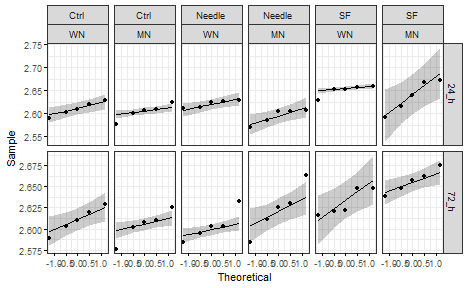
\includegraphics[width=0.95\linewidth,]{Statistics_report_files/figure-latex/qq-plot-figure-1b-c-myeloid-cells-1} 

}

\caption{Fig.1b-c-1: QQ-plots of myeloid cell counts split into groups by predictor variables}\label{fig:qq-plot-figure-1b-c-myeloid-cells}
\end{figure}

\subparagraph{Neutrophils}\label{neutrophils}

In spite of assessment limitations due to small group sizes, We concluded based on Shpiro-Wilks test (Table 2) and QQ-pots (Fig.1b-c-2) that all groups of the dataset were approximately normal distributed.

\begin{longtable}{ccclrrl}
\caption*{
{\large \textbf{Appendix Table 2}} \\ 
{\small \textbf{Neutrophils: Univariate Shapito-Wilks test results}}
} \\ 
\toprule
Diet & Route & Time\_point & variable & statistic & p & Outcome \\ 
\midrule\addlinespace[2.5pt]
WN & Ctrl & 24\_h & Counts & 0.9133 & 0.4879 & ns \\ 
WN & Ctrl & 72\_h & Counts & 0.9133 & 0.4879 & ns \\ 
MN & Ctrl & 24\_h & Counts & 0.9609 & 0.8144 & ns \\ 
MN & Ctrl & 72\_h & Counts & 0.9609 & 0.8144 & ns \\ 
WN & Needle & 24\_h & Counts & 0.8948 & 0.3818 & ns \\ 
WN & Needle & 72\_h & Counts & 0.9849 & 0.9590 & ns \\ 
MN & Needle & 24\_h & Counts & 0.8150 & 0.1068 & ns \\ 
MN & Needle & 72\_h & Counts & 0.9745 & 0.9032 & ns \\ 
WN & SF & 24\_h & Counts & 0.7958 & 0.0748 & ns \\ 
WN & SF & 72\_h & Counts & 0.9210 & 0.5361 & ns \\ 
MN & SF & 24\_h & Counts & 0.8692 & 0.2632 & ns \\ 
MN & SF & 72\_h & Counts & 0.9840 & 0.9547 & ns \\ 
\bottomrule
\end{longtable}

\begin{figure}[H]

{\centering 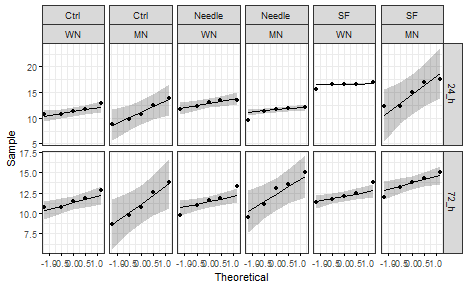
\includegraphics[width=0.95\linewidth,]{Statistics_report_files/figure-latex/qq-plot-figure-1b-c-neutrophils-1} 

}

\caption{Fig.1b-c-2: QQ-plots of neutrophil counts split into groups by predictor variables}\label{fig:qq-plot-figure-1b-c-neutrophils}
\end{figure}

\subparagraph{Monocytes}\label{monocytes}

In spite of assessment limitations due to small group sizes, We concluded based on Shpiro-Wilks test (Table 3) and QQ-pots (Fig.1b-c-3) that all groups of the myeloid cell dataset were approximately normal distributed.

\begin{longtable}{ccclrrl}
\caption*{
{\large \textbf{Appendix Table 3}} \\ 
{\small \textbf{Monocytes: Univariate Shapito-Wilks test results}}
} \\ 
\toprule
Diet & Route & Time\_point & variable & statistic & p & Outcome \\ 
\midrule\addlinespace[2.5pt]
WN & Ctrl & 24\_h & Counts & 0.8597 & 0.2271 & ns \\ 
WN & Ctrl & 72\_h & Counts & 0.8597 & 0.2271 & ns \\ 
MN & Ctrl & 24\_h & Counts & 0.8517 & 0.1999 & ns \\ 
MN & Ctrl & 72\_h & Counts & 0.8517 & 0.1999 & ns \\ 
WN & Needle & 24\_h & Counts & 0.8945 & 0.3803 & ns \\ 
WN & Needle & 72\_h & Counts & 0.9625 & 0.8250 & ns \\ 
MN & Needle & 24\_h & Counts & 0.9079 & 0.4552 & ns \\ 
MN & Needle & 72\_h & Counts & 0.9435 & 0.6907 & ns \\ 
WN & SF & 24\_h & Counts & 0.9944 & 0.9927 & ns \\ 
WN & SF & 72\_h & Counts & 0.8455 & 0.1806 & ns \\ 
MN & SF & 24\_h & Counts & 0.9226 & 0.5466 & ns \\ 
MN & SF & 72\_h & Counts & 0.9595 & 0.8048 & ns \\ 
\bottomrule
\end{longtable}

\begin{figure}[H]

{\centering 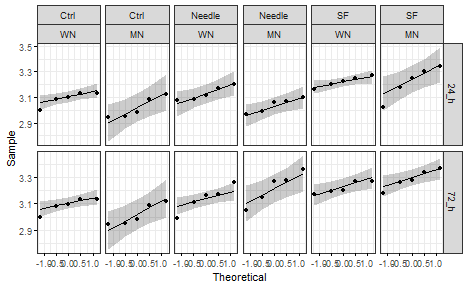
\includegraphics[width=0.95\linewidth,]{Statistics_report_files/figure-latex/qq-plot-figure-1b-c-monocytes-1} 

}

\caption{Fig.1b-c-3: QQ-plots of monocyte counts split into groups by predictor variables}\label{fig:qq-plot-figure-1b-c-monocytes}
\end{figure}

\paragraph{Homogeneity of variance}\label{homogeneity-of-variance}

The assessment of homogeneity of variance was also conducted for myeloid cell, neutrophil and monocyte counts separately. We employed a Levene's test for the whole model for each dataset. The p-value for the test suggested that the assumption of homogeneity of variance held for Myeloid\_cells (p=0.5236), held for Neutrophils (p=0.0502), and held for Monocytes (p=0.7728).

\paragraph{Outliers}\label{outliers}

It can be difficult to determine outliers in small datasets reliably as the analysis is dependent on the interquartile range of the data per group. We attempted it anyway and found 8 outliers in the Myeloid\_cells dataset (Table 4), 5 outliers in the Neutrophils dataset (Table 5), and 3 outliers in the Monocytes dataset (Table 6).

\begin{longtable}{ccccc}
\caption*{
{\large \textbf{Appendix Table 4}} \\ 
{\small \textbf{Myeloid cells: List of possible outliers}}
} \\ 
\toprule
Diet & Route & Time\_point & is.outlier & is.extreme \\ 
\midrule\addlinespace[2.5pt]
MN & Ctrl & 24\_h & TRUE & FALSE \\ 
MN & Ctrl & 24\_h & TRUE & FALSE \\ 
MN & Ctrl & 72\_h & TRUE & FALSE \\ 
MN & Ctrl & 72\_h & TRUE & FALSE \\ 
WN & Needle & 72\_h & TRUE & TRUE \\ 
MN & Needle & 72\_h & TRUE & FALSE \\ 
MN & Needle & 72\_h & TRUE & FALSE \\ 
WN & SF & 24\_h & TRUE & TRUE \\ 
\bottomrule
\end{longtable}

\begin{longtable}{ccccc}
\caption*{
{\large \textbf{Appendix Table 5}} \\ 
{\small \textbf{Neutrophils: List of possible outliers}}
} \\ 
\toprule
Diet & Route & Time\_point & is.outlier & is.extreme \\ 
\midrule\addlinespace[2.5pt]
WN & Needle & 72\_h & TRUE & FALSE \\ 
MN & Needle & 24\_h & TRUE & TRUE \\ 
WN & SF & 24\_h & TRUE & TRUE \\ 
WN & SF & 24\_h & TRUE & FALSE \\ 
WN & SF & 72\_h & TRUE & FALSE \\ 
\bottomrule
\end{longtable}

\begin{longtable}{ccccc}
\caption*{
{\large \textbf{Appendix Table 6}} \\ 
{\small \textbf{Monocytes: List of possible outliers}}
} \\ 
\toprule
Diet & Route & Time\_point & is.outlier & is.extreme \\ 
\midrule\addlinespace[2.5pt]
WN & Ctrl & 24\_h & TRUE & FALSE \\ 
WN & Ctrl & 72\_h & TRUE & FALSE \\ 
WN & Needle & 72\_h & TRUE & FALSE \\ 
\bottomrule
\end{longtable}

\subsubsection{Three-way analysis}\label{three-way-analysis}

\paragraph{Myeloid\_cells}\label{myeloid_cells-1}

Based on the assumption analysis, we decided to apply a Robust three-way ANOVA to the Myeloid\_cells dataset to determine the effects of ``Diet'', infection ``Route'' and time post infection (``Time\_point'') on the Myeloid\_cells count per pooled ear single-cell suspension (Table 7). The test output showed that only the ``Route'' predictor was a statistically significant factor, while the interaction between Time\_point and Diet was statistically significant, too.

\begin{longtable}{l|rrc}
\caption*{
{\large \textbf{Appendix Table 7}} \\ 
{\small \textbf{Myeloid cells: Robust three-way ANOVA}}
} \\ 
\toprule
\multicolumn{1}{l}{Predictors} & value & p.value & sig. \\ 
\midrule\addlinespace[2.5pt]
Diet & 0.0048 & 0.9500 & ns \\ 
Route & 29.5689 & 0.0007 & *** \\ 
Time\_point & 0.0447 & 0.8390 & ns \\ 
Diet:Route & 0.7681 & 0.7120 & ns \\ 
Diet:Time\_point & 7.4482 & 0.0230 & * \\ 
Route:Time\_point & 0.2226 & 0.9040 & ns \\ 
Diet:Route:Time\_point & 7.4542 & 0.0720 & + \\ 
\bottomrule
\end{longtable}

We looked for main effects by splitting the data by each predictor separately and analyzed the respective remaining two predictor by a Robust two-way ANOVA. The results showed that, after adjustment of p-values for multiple tests, only the ``Route'' predictor produced statistically significant p-values, regardless of whether the data was split by ``Diet'' or ``Time-point'' (Table 8). This suggested that the only predictor of impact on cell counts was the route of infection.

\begin{longtable}{l|lrrcrc}
\caption*{
{\large \textbf{Appendix Table 8}} \\ 
{\small \textbf{Myeloid cells: Robust two-way ANOVA}}
} \\ 
\toprule
\multicolumn{1}{l}{Grouper} & Predictor & value & p.value & Sig. & p.value.adj & sig. \\ 
\midrule\addlinespace[2.5pt]
\multicolumn{7}{l}{Grouped by Route} \\ 
\midrule\addlinespace[2.5pt]
Ctrl & Diet & 0.7025 & 0.415 & ns & 0.5810 & ns \\ 
Ctrl & Time\_point & 0.0000 & 0.999 & ns & 0.9990 & ns \\ 
Ctrl & Diet:Time\_point & 0.0000 & 0.999 & ns & 0.9990 & ns \\ 
Needle & Diet & 0.1500 & 0.707 & ns & 0.8248 & ns \\ 
Needle & Time\_point & 0.4370 & 0.523 & ns & 0.6510 & ns \\ 
Needle & Diet:Time\_point & 6.7428 & 0.024 & * & 0.1008 & ns \\ 
SF & Diet & 0.4354 & 0.527 & ns & 0.6510 & ns \\ 
SF & Time\_point & 0.0015 & 0.971 & ns & 0.9990 & ns \\ 
SF & Diet:Time\_point & 4.1861 & 0.069 & + & 0.1701 & ns \\ 
\midrule\addlinespace[2.5pt]
\multicolumn{7}{l}{Grouped by Diet} \\ 
\midrule\addlinespace[2.5pt]
WN & Route & 28.0464 & 0.001 & *** & 0.0105 & * \\ 
WN & Time\_point & 5.2407 & 0.032 & * & 0.1120 & ns \\ 
WN & Route:Time\_point & 2.5384 & 0.326 & ns & 0.5444 & ns \\ 
MN & Route & 19.2056 & 0.003 & ** & 0.0210 & * \\ 
MN & Time\_point & 3.5769 & 0.076 & + & 0.1701 & ns \\ 
MN & Route:Time\_point & 2.5075 & 0.337 & ns & 0.5444 & ns \\ 
\midrule\addlinespace[2.5pt]
\multicolumn{7}{l}{Grouped by Time\_point} \\ 
\midrule\addlinespace[2.5pt]
24\_h & Diet & 4.6264 & 0.050 & * & 0.1500 & ns \\ 
24\_h & Route & 17.3213 & 0.004 & ** & 0.0210 & * \\ 
24\_h & Diet:Route & 2.3091 & 0.368 & ns & 0.5520 & ns \\ 
72\_h & Diet & 3.3991 & 0.081 & + & 0.1701 & ns \\ 
72\_h & Route & 29.3554 & 0.001 & *** & 0.0105 & * \\ 
72\_h & Diet:Route & 5.2718 & 0.112 & ns & 0.2138 & ns \\ 
\bottomrule
\end{longtable}

For the analysis of the simple simple main effect for each respective predictor, we performed Robust one-way ANOVA with individual predictors of the data split by the other two predictors. The output showed yet again that after the adjustment of p-values for multiple tests, only the ``Route'' predictor produce statistically significant p-values (Table 9). Here, the differences were observed in the well-nourished group (WN) at 24 h post infection and for the malnourished group at 72 h post infection.

\begin{longtable}{lllrrrrrrc}
\caption*{
{\large \textbf{Appendix Table 9}} \\ 
{\small \textbf{Myeloid cells: Robust one-way ANOVA}}
} \\ 
\toprule
Predictor\_1 & Predictor\_2 & Effect & test & df1 & df2 & p.value & effsize & p.value.adj & sig. \\ 
\midrule\addlinespace[2.5pt]
\multicolumn{10}{l}{Predictor: Time\_point} \\ 
\midrule\addlinespace[2.5pt]
Ctrl & WN & Time\_point & 0.0000 & 1 & 8.0000 & 1.0000 & 0.0000 & 1.0000 & ns \\ 
Ctrl & MN & Time\_point & 0.0000 & 1 & 8.0000 & 1.0000 & 0.0000 & 1.0000 & ns \\ 
Needle & WN & Time\_point & 3.5282 & 1 & 5.5647 & 0.1132 & 0.7337 & 0.2033 & ns \\ 
Needle & MN & Time\_point & 3.6121 & 1 & 6.2598 & 0.1041 & 0.9017 & 0.2033 & ns \\ 
SF & WN & Time\_point & 4.8246 & 1 & 7.5253 & 0.0614 & 0.7261 & 0.1965 & ns \\ 
SF & MN & Time\_point & 1.3003 & 1 & 5.2694 & 0.3033 & 0.5259 & 0.4412 & ns \\ 
\midrule\addlinespace[2.5pt]
\multicolumn{10}{l}{Predictor: Diet} \\ 
\midrule\addlinespace[2.5pt]
24\_h & Ctrl & Diet & 0.3512 & 1 & 7.8195 & 0.5702 & 0.2800 & 0.6516 & ns \\ 
24\_h & Needle & Diet & 10.1859 & 1 & 5.9402 & 0.0191 & 0.9926 & 0.1017 & ns \\ 
24\_h & SF & Diet & 0.6400 & 1 & 4.9962 & 0.4600 & 0.3842 & 0.6134 & ns \\ 
72\_h & Ctrl & Diet & 0.3512 & 1 & 7.8195 & 0.5702 & 0.2800 & 0.6516 & ns \\ 
72\_h & Needle & Diet & 1.5616 & 1 & 6.7245 & 0.2532 & 0.5753 & 0.4051 & ns \\ 
72\_h & SF & Diet & 7.3397 & 1 & 7.8679 & 0.0271 & 0.8992 & 0.1084 & ns \\ 
\midrule\addlinespace[2.5pt]
\multicolumn{10}{l}{Predictor: Route} \\ 
\midrule\addlinespace[2.5pt]
24\_h & WN & Route & 12.5661 & 2 & 7.4933 & 0.0040 & 0.9018 & 0.0323 & * \\ 
24\_h & MN & Route & 2.9293 & 2 & 7.5513 & 0.1144 & 0.6507 & 0.2033 & ns \\ 
72\_h & WN & Route & 3.3900 & 2 & 7.9569 & 0.0861 & 0.6194 & 0.2033 & ns \\ 
72\_h & MN & Route & 12.7031 & 2 & 7.4981 & 0.0039 & 0.7858 & 0.0323 & * \\ 
\bottomrule
\end{longtable}

For the pairwise comparison, we applied a Linear contrast expression. The output showed that at 24 h post infection, the sand fly infection route was statistically significant from the control and needle inoculum in the well-nourished (WN) group (Table 10). At 72 h, the sand fly infection route was statistically significant from the control in the malnourished group. Further, statistically significant difference were observed between well-nourished and malnourished mice inoculated by needle at 24 h post infection and infected by sand fly at 72 h post infection.

\begin{longtable}{llccrrrrc}
\caption*{
{\large \textbf{Appendix Table 10}} \\ 
{\small \textbf{Myeloid cells: Pairwise comparison by Linear Contrast Expression}}
} \\ 
\toprule
Predictor\_1 & Predictor\_2 & Group & Group.1 & psihat & ci.lower & ci.upper & p.value & Sig. \\ 
\midrule\addlinespace[2.5pt]
\multicolumn{9}{l}{Predictor: Time\_point} \\ 
\midrule\addlinespace[2.5pt]
Ctrl & WN & 24\_h & 72\_h & 0.0000 & -0.0224 & 0.0224 & 1.0000 & ns \\ 
Ctrl & MN & 24\_h & 72\_h & 0.0000 & -0.0261 & 0.0261 & 1.0000 & ns \\ 
Needle & WN & 24\_h & 72\_h & 0.0169 & -0.0055 & 0.0394 & 0.1132 & ns \\ 
Needle & MN & 24\_h & 72\_h & -0.0285 & -0.0647 & 0.0078 & 0.1041 & ns \\ 
SF & WN & 24\_h & 72\_h & 0.0197 & -0.0012 & 0.0406 & 0.0614 & + \\ 
SF & MN & 24\_h & 72\_h & -0.0190 & -0.0611 & 0.0231 & 0.3033 & ns \\ 
\midrule\addlinespace[2.5pt]
\multicolumn{9}{l}{Predictor: Diet} \\ 
\midrule\addlinespace[2.5pt]
24\_h & Ctrl & WN & MN & 0.0062 & -0.0182 & 0.0306 & 0.5702 & ns \\ 
24\_h & Needle & WN & MN & 0.0261 & 0.0060 & 0.0461 & 0.0191 & * \\ 
24\_h & SF & WN & MN & 0.0131 & -0.0290 & 0.0552 & 0.4600 & ns \\ 
72\_h & Ctrl & WN & MN & 0.0062 & -0.0182 & 0.0306 & 0.5702 & ns \\ 
72\_h & Needle & WN & MN & -0.0193 & -0.0561 & 0.0175 & 0.2532 & ns \\ 
72\_h & SF & WN & MN & -0.0256 & -0.0474 & -0.0037 & 0.0271 & * \\ 
\midrule\addlinespace[2.5pt]
\multicolumn{9}{l}{Predictor: Route} \\ 
\midrule\addlinespace[2.5pt]
24\_h & WN & Ctrl & Needle & -0.0103 & -0.0350 & 0.0144 & 0.2350 & ns \\ 
24\_h & WN & Ctrl & SF & -0.0403 & -0.0666 & -0.0140 & 0.0040 & ** \\ 
24\_h & WN & Needle & SF & -0.0300 & -0.0502 & -0.0098 & 0.0040 & ** \\ 
24\_h & MN & Ctrl & Needle & 0.0096 & -0.0225 & 0.0416 & 0.4028 & ns \\ 
24\_h & MN & Ctrl & SF & -0.0334 & -0.0888 & 0.0220 & 0.1542 & ns \\ 
24\_h & MN & Needle & SF & -0.0430 & -0.0983 & 0.0123 & 0.1421 & ns \\ 
72\_h & WN & Ctrl & Needle & 0.0066 & -0.0253 & 0.0385 & 0.5523 & ns \\ 
72\_h & WN & Ctrl & SF & -0.0206 & -0.0498 & 0.0087 & 0.1060 & ns \\ 
72\_h & WN & Needle & SF & -0.0272 & -0.0595 & 0.0050 & 0.1060 & ns \\ 
72\_h & MN & Ctrl & Needle & -0.0189 & -0.0665 & 0.0287 & 0.2597 & ns \\ 
72\_h & MN & Ctrl & SF & -0.0524 & -0.0828 & -0.0219 & 0.0031 & ** \\ 
72\_h & MN & Needle & SF & -0.0335 & -0.0804 & 0.0135 & 0.0936 & + \\ 
\bottomrule
\end{longtable}

\paragraph{Neutrophils}\label{neutrophils-1}

Based on the assumption analysis, we decided to apply a Robust three-way ANOVA to the Neutrophils dataset to determine the effects of ``Diet'', infection ``Route'' and time post infection (``Time\_point'') on the Neutrophils count per pooled ear single-cell suspension (Table 11). The test output showed that only the ``Route'' predictor was a statistically significant factor, while the interaction between Time\_point and Diet was statistically significant, too. Thus, Neutrophils followed the same pattern as the overarching Myeloid\_cells category.

\begin{longtable}{l|rrc}
\caption*{
{\large \textbf{Appendix Table 11}} \\ 
{\small \textbf{Neutrophils: Robust three-way ANOVA}}
} \\ 
\toprule
\multicolumn{1}{l}{Predictors} & value & p.value & sig. \\ 
\midrule\addlinespace[2.5pt]
Diet & 0.1394 & 0.720 & ns \\ 
Route & 23.0377 & 0.004 & ** \\ 
Time\_point & 4.3763 & 0.065 & + \\ 
Diet:Route & 0.0479 & 0.979 & ns \\ 
Diet:Time\_point & 4.0582 & 0.074 & + \\ 
Route:Time\_point & 5.4366 & 0.150 & ns \\ 
Diet:Route:Time\_point & 1.9427 & 0.458 & ns \\ 
\bottomrule
\end{longtable}

We looked for main effects by splitting the data by each predictor separately and analyzed the respective remaining two predictor by a Robust two-way ANOVA. After adjustment of p-values for multiple tests, We observed statistically significant differences between 24 h and 72 h post infection, when the data was split by infestation route; in well-nourished group for Route, Time\_point and their interaction, as much as for infection route in the malnourished group, when the data was split by ``Diet''; and for infection routes at 24 h post infection, when the data was split by Time\_point (Table 12).

\begin{longtable}{l|lrrcrc}
\caption*{
{\large \textbf{Appendix Table 12}} \\ 
{\small \textbf{Neutrophils: Robust two-way ANOVA}}
} \\ 
\toprule
\multicolumn{1}{l}{Grouper} & Predictor & value & p.value & Sig. & p.value.adj & sig. \\ 
\midrule\addlinespace[2.5pt]
\multicolumn{7}{l}{Grouped by Route} \\ 
\midrule\addlinespace[2.5pt]
Ctrl & Diet & 0.3205 & 0.583 & ns & 0.8745 & ns \\ 
Ctrl & Time\_point & 0.0000 & 0.999 & ns & 0.9990 & ns \\ 
Ctrl & Diet:Time\_point & 0.0000 & 0.999 & ns & 0.9990 & ns \\ 
Needle & Diet & 0.1839 & 0.678 & ns & 0.8899 & ns \\ 
Needle & Time\_point & 0.0428 & 0.841 & ns & 0.9812 & ns \\ 
Needle & Diet:Time\_point & 3.7795 & 0.078 & + & 0.1638 & ns \\ 
SF & Diet & 0.0473 & 0.834 & ns & 0.9812 & ns \\ 
SF & Time\_point & 16.1728 & 0.003 & ** & 0.0126 & * \\ 
SF & Diet:Time\_point & 5.0287 & 0.053 & + & 0.1237 & ns \\ 
\midrule\addlinespace[2.5pt]
\multicolumn{7}{l}{Grouped by Diet} \\ 
\midrule\addlinespace[2.5pt]
WN & Route & 68.7607 & 0.001 & *** & 0.0053 & ** \\ 
WN & Time\_point & 31.4785 & 0.001 & *** & 0.0053 & ** \\ 
WN & Route:Time\_point & 34.6536 & 0.001 & *** & 0.0053 & ** \\ 
MN & Route & 13.4578 & 0.009 & ** & 0.0315 & * \\ 
MN & Time\_point & 0.0021 & 0.964 & ns & 0.9990 & ns \\ 
MN & Route:Time\_point & 1.9351 & 0.423 & ns & 0.6833 & ns \\ 
\midrule\addlinespace[2.5pt]
\multicolumn{7}{l}{Grouped by Time\_point} \\ 
\midrule\addlinespace[2.5pt]
24\_h & Diet & 4.6992 & 0.050 & * & 0.1237 & ns \\ 
24\_h & Route & 37.4309 & 0.001 & *** & 0.0053 & ** \\ 
24\_h & Diet:Route & 0.9951 & 0.644 & ns & 0.8899 & ns \\ 
72\_h & Diet & 1.3219 & 0.267 & ns & 0.5097 & ns \\ 
72\_h & Route & 8.1667 & 0.046 & * & 0.1237 & ns \\ 
72\_h & Diet:Route & 2.1155 & 0.395 & ns & 0.6833 & ns \\ 
\bottomrule
\end{longtable}

For the analysis of the simple simple main effect for each respective predictor, we performed Robust one-way ANOVA with individual predictors of the data split by the other two predictors. The output showed statistically significant p-values for the sand fly inoculation in the well-nourished group for the Time\_point predictor and at 24 h post infection in the well-nourished group for the infection route (Table 13).

\begin{longtable}{lllrrrlrrc}
\caption*{
{\large \textbf{Appendix Table 13}} \\ 
{\small \textbf{Neutrophils: Robust one-way ANOVA}}
} \\ 
\toprule
Predictor\_1 & Predictor\_2 & Effect & test & df1 & df2 & p.value & effsize & p.value.adj & sig. \\ 
\midrule\addlinespace[2.5pt]
\multicolumn{10}{l}{Predictor: Time\_point} \\ 
\midrule\addlinespace[2.5pt]
Ctrl & WN & Time\_point & 0.0000 & 1 & 8.0000 & 1.0000 & 0.0000 & 1.0000 & ns \\ 
Ctrl & MN & Time\_point & 0.0000 & 1 & 8.0000 & 1.0000 & 0.0000 & 1.0000 & ns \\ 
Needle & WN & Time\_point & 4.1593 & 1 & 6.4828 & 0.0840 & 0.8107 & 0.2240 & ns \\ 
Needle & MN & Time\_point & 1.0452 & 1 & 5.6120 & 0.3486 & 0.4543 & 0.5706 & ns \\ 
SF & WN & Time\_point & 76.4341 & 1 & 5.6989 & 0.0002 & 1.0898 & 0.0013 & ** \\ 
SF & MN & Time\_point & 0.9078 & 1 & 5.5609 & 0.3803 & 0.3810 & 0.5706 & ns \\ 
\midrule\addlinespace[2.5pt]
\multicolumn{10}{l}{Predictor: Diet} \\ 
\midrule\addlinespace[2.5pt]
24\_h & Ctrl & Diet & 0.1603 & 1 & 5.3717 & 0.7043 & 0.1989 & 0.8050 & ns \\ 
24\_h & Needle & Diet & 7.1359 & 1 & 7.4476 & 0.0302 & 1.0777 & 0.1609 & ns \\ 
24\_h & SF & Diet & 2.0228 & 1 & 4.2581 & 0.2239 & 0.5190 & 0.4478 & ns \\ 
72\_h & Ctrl & Diet & 0.1603 & 1 & 5.3717 & 0.7043 & 0.1989 & 0.8050 & ns \\ 
72\_h & Needle & Diet & 0.7151 & 1 & 6.4714 & 0.4279 & 0.3795 & 0.5706 & ns \\ 
72\_h & SF & Diet & 4.0661 & 1 & 7.7816 & 0.0795 & 0.7530 & 0.2240 & ns \\ 
\midrule\addlinespace[2.5pt]
\multicolumn{10}{l}{Predictor: Route} \\ 
\midrule\addlinespace[2.5pt]
24\_h & WN & Route & 78.7826 & 2 & 7.3614 & <0.0001 & 0.9442 & 0.0002 & *** \\ 
24\_h & MN & Route & 3.9055 & 2 & 6.8243 & 0.0740 & 0.7267 & 0.2240 & ns \\ 
72\_h & WN & Route & 0.9855 & 2 & 7.8365 & 0.4152 & 0.4338 & 0.5706 & ns \\ 
72\_h & MN & Route & 2.7786 & 2 & 7.2716 & 0.1269 & 0.5443 & 0.2901 & ns \\ 
\bottomrule
\end{longtable}

For the pairwise comparison, we applied a Linear contrast expression. The output showed that at 24 h post infection, there were statistically significant differences at 24 h post infection between the well-nourished and malnourished groups for the needle inoculum and at 72 h post infection for the sand fly inoculation (Table 14). Further, we observed differences in the well-nourished group at 24 h post infection between the sand fly inoculum and both, the control and needle inoculum. For the malnourished group we observed statistically significant p-values at 72 h post infection between the sand fly inolculum and the control group.

\begin{longtable}{llccrrrrc}
\caption*{
{\large \textbf{Appendix Table 14}} \\ 
{\small \textbf{Neutrophils: Pairwise comparison by Linear Contrast Expression}}
} \\ 
\toprule
Predictor\_1 & Predictor\_2 & Group & Group.1 & psihat & ci.lower & ci.upper & p.value & Sig. \\ 
\midrule\addlinespace[2.5pt]
\multicolumn{9}{l}{Predictor: Time\_point} \\ 
\midrule\addlinespace[2.5pt]
Ctrl & WN & 24\_h & 72\_h & 0.0000 & -1.2773 & 1.2773 & 1.0000 & ns \\ 
Ctrl & MN & 24\_h & 72\_h & 0.0000 & -3.0375 & 3.0375 & 1.0000 & ns \\ 
Needle & WN & 24\_h & 72\_h & 1.3539 & -0.2416 & 2.9494 & 0.0840 & + \\ 
Needle & MN & 24\_h & 72\_h & -1.0936 & -3.7554 & 1.5683 & 0.3486 & ns \\ 
SF & WN & 24\_h & 72\_h & 4.1934 & 3.0045 & 5.3822 & 0.0002 & *** \\ 
SF & MN & 24\_h & 72\_h & 1.1910 & -1.9272 & 4.3091 & 0.3803 & ns \\ 
\midrule\addlinespace[2.5pt]
\multicolumn{9}{l}{Predictor: Diet} \\ 
\midrule\addlinespace[2.5pt]
24\_h & Ctrl & WN & MN & 0.4045 & -2.1397 & 2.9487 & 0.7043 & ns \\ 
24\_h & Needle & WN & MN & 1.4936 & 0.1874 & 2.7999 & 0.0302 & * \\ 
24\_h & SF & WN & MN & 1.6467 & -1.4926 & 4.7860 & 0.2239 & ns \\ 
72\_h & Ctrl & WN & MN & 0.4045 & -2.1397 & 2.9487 & 0.7043 & ns \\ 
72\_h & Needle & WN & MN & -0.9538 & -3.6657 & 1.7581 & 0.4279 & ns \\ 
72\_h & SF & WN & MN & -1.3556 & -2.9135 & 0.2023 & 0.0795 & + \\ 
\midrule\addlinespace[2.5pt]
\multicolumn{9}{l}{Predictor: Route} \\ 
\midrule\addlinespace[2.5pt]
24\_h & WN & Ctrl & Needle & -1.3581 & -2.8960 & 0.1798 & 0.0309 & * \\ 
24\_h & WN & Ctrl & SF & -4.9856 & -6.3932 & -3.5781 & 0.0001 & **** \\ 
24\_h & WN & Needle & SF & -3.6276 & -4.8538 & -2.4014 & 0.0001 & **** \\ 
24\_h & MN & Ctrl & Needle & -0.2689 & -3.6094 & 3.0716 & 0.8036 & ns \\ 
24\_h & MN & Ctrl & SF & -3.7434 & -8.1407 & 0.6539 & 0.0534 & + \\ 
24\_h & MN & Needle & SF & -3.4745 & -7.5673 & 0.6183 & 0.0534 & + \\ 
72\_h & WN & Ctrl & Needle & -0.0042 & -2.1190 & 2.1106 & 0.9953 & ns \\ 
72\_h & WN & Ctrl & SF & -0.7923 & -2.5263 & 0.9418 & 0.4595 & ns \\ 
72\_h & WN & Needle & SF & -0.7881 & -2.9489 & 1.3727 & 0.4595 & ns \\ 
72\_h & MN & Ctrl & Needle & -1.3625 & -5.3495 & 2.6245 & 0.3412 & ns \\ 
72\_h & MN & Ctrl & SF & -2.5524 & -5.9102 & 0.8053 & 0.1555 & ns \\ 
72\_h & MN & Needle & SF & -1.1900 & -4.6858 & 2.3059 & 0.3412 & ns \\ 
\bottomrule
\end{longtable}

\paragraph{Monocytes}\label{monocytes-1}

Based on the assumption analysis, we decided to apply a Robust three-way ANOVA to the Monocytes dataset to determine the effects of ``Diet'', infection ``Route'' and time post infection (``Time\_point'') on the Monocytes count per pooled ear single-cell suspension (Table 15). The test output showed that only the ``Route'' predictor was a statistically significant factor. No statistically significant interaction between any predictors was observed.

\begin{longtable}{l|rrc}
\caption*{
{\large \textbf{Appendix Table 15}} \\ 
{\small \textbf{Monocytes: Robust three-way ANOVA}}
} \\ 
\toprule
\multicolumn{1}{l}{Predictors} & value & p.value & sig. \\ 
\midrule\addlinespace[2.5pt]
Diet & 0.4677 & 0.5100 & ns \\ 
Route & 47.2342 & 0.0001 & **** \\ 
Time\_point & 3.5637 & 0.0760 & + \\ 
Diet:Route & 6.4411 & 0.0830 & + \\ 
Diet:Time\_point & 2.4362 & 0.1370 & ns \\ 
Route:Time\_point & 3.9590 & 0.1950 & ns \\ 
Diet:Route:Time\_point & 2.2057 & 0.3830 & ns \\ 
\bottomrule
\end{longtable}

We looked for main effects by splitting the data by each predictor separately and analyzed the respective remaining two predictor by a Robust two-way ANOVA. The results showed that, after adjustment of p-values for multiple tests, only the ``Route'' predictor produced statistically significant p-values, regardless of whether the data was split by ``Diet'' or ``Time-point'' (Table 16). This suggested that the only predictor of impact on cell counts was the route of infection. No statistically significant interactions were observed at this level.

\begin{longtable}{l|lrrcrc}
\caption*{
{\large \textbf{Appendix Table 16}} \\ 
{\small \textbf{Monovytes: Robust two-way ANOVA}}
} \\ 
\toprule
\multicolumn{1}{l}{Grouper} & Predictor & value & p.value & Sig. & p.value.adj & sig. \\ 
\midrule\addlinespace[2.5pt]
\multicolumn{7}{l}{Grouped by Route} \\ 
\midrule\addlinespace[2.5pt]
Ctrl & Diet & 5.2338 & 0.037 & * & 0.1110 & ns \\ 
Ctrl & Time\_point & 0.0000 & 0.999 & ns & 0.9990 & ns \\ 
Ctrl & Diet:Time\_point & 0.0000 & 0.999 & ns & 0.9990 & ns \\ 
Needle & Diet & 0.0138 & 0.909 & ns & 0.9990 & ns \\ 
Needle & Time\_point & 6.2017 & 0.027 & * & 0.0945 & + \\ 
Needle & Diet:Time\_point & 4.8351 & 0.047 & * & 0.1234 & ns \\ 
SF & Diet & 0.7354 & 0.413 & ns & 0.5964 & ns \\ 
SF & Time\_point & 0.7811 & 0.399 & ns & 0.5964 & ns \\ 
SF & Diet:Time\_point & 0.8265 & 0.387 & ns & 0.5964 & ns \\ 
\midrule\addlinespace[2.5pt]
\multicolumn{7}{l}{Grouped by Diet} \\ 
\midrule\addlinespace[2.5pt]
WN & Route & 36.6533 & 0.001 & *** & 0.0070 & ** \\ 
WN & Time\_point & 0.0245 & 0.878 & ns & 0.9990 & ns \\ 
WN & Route:Time\_point & 0.0477 & 0.978 & ns & 0.9990 & ns \\ 
MN & Route & 32.3071 & 0.001 & *** & 0.0070 & ** \\ 
MN & Time\_point & 5.9000 & 0.025 & * & 0.0945 & + \\ 
MN & Route:Time\_point & 5.5106 & 0.107 & ns & 0.2043 & ns \\ 
\midrule\addlinespace[2.5pt]
\multicolumn{7}{l}{Grouped by Time\_point} \\ 
\midrule\addlinespace[2.5pt]
24\_h & Diet & 3.9779 & 0.065 & + & 0.1517 & ns \\ 
24\_h & Route & 21.9364 & 0.002 & ** & 0.0105 & * \\ 
24\_h & Diet:Route & 1.6608 & 0.478 & ns & 0.6274 & ns \\ 
72\_h & Diet & 0.6652 & 0.426 & ns & 0.5964 & ns \\ 
72\_h & Route & 46.8385 & 0.001 & *** & 0.0070 & ** \\ 
72\_h & Diet:Route & 6.2872 & 0.078 & + & 0.1638 & ns \\ 
\bottomrule
\end{longtable}

For the analysis of the simple simple main effect for each respective predictor, we performed Robust one-way ANOVA with individual predictors of the data split by the other two predictors. The output showed that after the adjustment of p-values for multiple tests, only the ``Route'' predictor produce statistically significant p-values in the malnourished group at 72 h post infection (Table 17).

\begin{longtable}{lllrrrrrrc}
\caption*{
{\large \textbf{Appendix Table 17}} \\ 
{\small \textbf{Monocytes: Robust one-way ANOVA}}
} \\ 
\toprule
Predictor\_1 & Predictor\_2 & Effect & test & df1 & df2 & p.value & effsize & p.value.adj & sig. \\ 
\midrule\addlinespace[2.5pt]
\multicolumn{10}{l}{Predictor: Time\_point} \\ 
\midrule\addlinespace[2.5pt]
Ctrl & WN & Time\_point & 0.0000 & 1 & 8.0000 & 1.0000 & 0.0000 & 1.0000 & ns \\ 
Ctrl & MN & Time\_point & 0.0000 & 1 & 8.0000 & 1.0000 & 0.0000 & 1.0000 & ns \\ 
Needle & WN & Time\_point & 0.0512 & 1 & 6.2708 & 0.8281 & 0.1320 & 1.0000 & ns \\ 
Needle & MN & Time\_point & 9.3895 & 1 & 5.7100 & 0.0236 & 0.9343 & 0.0942 & + \\ 
SF & WN & Time\_point & 0.0010 & 1 & 7.9009 & 0.9756 & 0.0126 & 1.0000 & ns \\ 
SF & MN & Time\_point & 0.9577 & 1 & 6.3626 & 0.3635 & 0.5490 & 0.5287 & ns \\ 
\midrule\addlinespace[2.5pt]
\multicolumn{10}{l}{Predictor: Diet} \\ 
\midrule\addlinespace[2.5pt]
24\_h & Ctrl & Diet & 2.6169 & 1 & 7.0286 & 0.1496 & 0.5569 & 0.2659 & ns \\ 
24\_h & Needle & Diet & 6.5185 & 1 & 7.9850 & 0.0341 & 0.8413 & 0.1090 & ns \\ 
24\_h & SF & Diet & 0.0009 & 1 & 4.8921 & 0.9767 & 0.0196 & 1.0000 & ns \\ 
72\_h & Ctrl & Diet & 2.6169 & 1 & 7.0286 & 0.1496 & 0.5569 & 0.2659 & ns \\ 
72\_h & Needle & Diet & 1.3637 & 1 & 7.6805 & 0.2779 & 0.5236 & 0.4446 & ns \\ 
72\_h & SF & Diet & 2.6348 & 1 & 6.9154 & 0.1491 & 0.6089 & 0.2659 & ns \\ 
\midrule\addlinespace[2.5pt]
\multicolumn{10}{l}{Predictor: Route} \\ 
\midrule\addlinespace[2.5pt]
24\_h & WN & Route & 9.5871 & 2 & 7.8674 & 0.0078 & 0.8982 & 0.0622 & + \\ 
24\_h & MN & Route & 4.6108 & 2 & 7.4049 & 0.0501 & 0.7502 & 0.1335 & ns \\ 
72\_h & WN & Route & 7.7990 & 2 & 7.5548 & 0.0145 & 0.6443 & 0.0776 & + \\ 
72\_h & MN & Route & 14.2513 & 2 & 7.7234 & 0.0026 & 0.7890 & 0.0409 & * \\ 
\bottomrule
\end{longtable}

For the pairwise comparison, we applied a Linear contrast expression. The output showed that at 24 h post infection, the sand fly infection route was statistically significant from the control and needle inoculum in the well-nourished (WN) group (Table 18). At 72 h, the sand fly infection route was statistically significant from the control in the malnourished group. Further, statistically significant difference were observed between well-nourished and malnourished mice inoculated by needle at 24 h post infection and infected by sand fly at 72 h post infection for the needle and sand fly inoculum, respectively.

\begin{longtable}{llccrrrrc}
\caption*{
{\large \textbf{Appendix Table 18}} \\ 
{\small \textbf{Monocytes: Pairwise comparison by Linear Contrast Expression}}
} \\ 
\toprule
Predictor\_1 & Predictor\_2 & Group & Group.1 & psihat & ci.lower & ci.upper & p.value & Sig. \\ 
\midrule\addlinespace[2.5pt]
\multicolumn{9}{l}{Predictor: Time\_point} \\ 
\midrule\addlinespace[2.5pt]
Ctrl & WN & 24\_h & 72\_h & 0.0000 & -0.0791 & 0.0791 & 1.0000 & ns \\ 
Ctrl & MN & 24\_h & 72\_h & 0.0000 & -0.1169 & 0.1169 & 1.0000 & ns \\ 
Needle & WN & 24\_h & 72\_h & -0.0114 & -0.1337 & 0.1108 & 0.8281 & ns \\ 
Needle & MN & 24\_h & 72\_h & -0.1838 & -0.3324 & -0.0352 & 0.0236 & * \\ 
SF & WN & 24\_h & 72\_h & 0.0009 & -0.0646 & 0.0664 & 0.9756 & ns \\ 
SF & MN & 24\_h & 72\_h & -0.0633 & -0.2195 & 0.0928 & 0.3635 & ns \\ 
\midrule\addlinespace[2.5pt]
\multicolumn{9}{l}{Predictor: Diet} \\ 
\midrule\addlinespace[2.5pt]
24\_h & Ctrl & WN & MN & 0.0700 & -0.0322 & 0.1722 & 0.1496 & ns \\ 
24\_h & Needle & WN & MN & 0.0908 & 0.0088 & 0.1728 & 0.0341 & * \\ 
24\_h & SF & WN & MN & 0.0018 & -0.1515 & 0.1551 & 0.9767 & ns \\ 
72\_h & Ctrl & WN & MN & 0.0700 & -0.0322 & 0.1722 & 0.1496 & ns \\ 
72\_h & Needle & WN & MN & -0.0816 & -0.2439 & 0.0807 & 0.2779 & ns \\ 
72\_h & SF & WN & MN & -0.0624 & -0.1535 & 0.0287 & 0.1491 & ns \\ 
\midrule\addlinespace[2.5pt]
\multicolumn{9}{l}{Predictor: Route} \\ 
\midrule\addlinespace[2.5pt]
24\_h & WN & Ctrl & Needle & -0.0393 & -0.1416 & 0.0629 & 0.2879 & ns \\ 
24\_h & WN & Ctrl & SF & -0.1324 & -0.2246 & -0.0401 & 0.0089 & ** \\ 
24\_h & WN & Needle & SF & -0.0930 & -0.1863 & 0.0002 & 0.0276 & * \\ 
24\_h & MN & Ctrl & Needle & -0.0185 & -0.1522 & 0.1152 & 0.6868 & ns \\ 
24\_h & MN & Ctrl & SF & -0.2005 & -0.4060 & 0.0049 & 0.0418 & * \\ 
24\_h & MN & Needle & SF & -0.1820 & -0.3834 & 0.0194 & 0.0418 & * \\ 
72\_h & WN & Ctrl & Needle & -0.0507 & -0.2096 & 0.1081 & 0.3508 & ns \\ 
72\_h & WN & Ctrl & SF & -0.1315 & -0.2271 & -0.0359 & 0.0109 & * \\ 
72\_h & WN & Needle & SF & -0.0807 & -0.2388 & 0.0774 & 0.2280 & ns \\ 
72\_h & MN & Ctrl & Needle & -0.2023 & -0.4017 & -0.0030 & 0.0258 & * \\ 
72\_h & MN & Ctrl & SF & -0.2638 & -0.4067 & -0.1210 & 0.0018 & ** \\ 
72\_h & MN & Needle & SF & -0.0615 & -0.2581 & 0.1351 & 0.3639 & ns \\ 
\bottomrule
\end{longtable}

\subsubsection{Statistical power}\label{statistical-power}

Considering the small group \emph{N}=5 and the low occurrence of statistical significant outcomes, it stood to reason that the study design was statistically underpowered by necessity to keep animal number and costs manageable. Thus, we performed a retrospective power analysis on the data by cell-type group to explore this.

\paragraph{\texorpdfstring{Effect size estimation based on partial eta\textsuperscript{2}}{Effect size estimation based on partial eta2}}\label{effect-size-estimation-based-on-partial-eta2}

Effect sizes were calculated by predictor and the different potential interaction combinations of them. Appendix tables 19 to 21 show the respective effect sizes. Note that upper ends of the confidence intervals were automatically set to 1 for this type of calculation. Large effect sizes reflected statistically meaningful differences in the data analysis. The partial eta\textsuperscript{2} values from the effect size calculation were then used to the retrospective power calculations.

\begin{longtable}{lrrrcl}
\caption*{
{\large \textbf{Appendix Table 19}} \\ 
{\small \textbf{Myeloid cells: Effect size estimation}}
} \\ 
\toprule
Parameter & Eta2\_partial & CI\_low & CI\_high & Effect\_size & Effect Size \\ 
\midrule\addlinespace[2.5pt]
Diet & 0.0073 & 0.0000 & 1 & very small & very small \\ 
Route & 0.5033 & 0.3277 & 1 & large & large \\ 
Time\_point & 0.0017 & 0.0000 & 1 & very small & very small \\ 
Diet:Route & 0.0398 & 0.0000 & 1 & small & small \\ 
Diet:Time\_point & 0.1270 & 0.0174 & 1 & small & medium \\ 
Route:Time\_point & 0.0125 & 0.0000 & 1 & very small & small \\ 
Diet:Route:Time\_point & 0.0689 & 0.0000 & 1 & small & medium \\ 
\bottomrule
\end{longtable}

\begin{longtable}{lrrrcl}
\caption*{
{\large \textbf{Appendix Table 20}} \\ 
{\small \textbf{Neutrophils: Effect size estimation}}
} \\ 
\toprule
Parameter & Eta2\_partial & CI\_low & CI\_high & Effect\_size & Effect Size \\ 
\midrule\addlinespace[2.5pt]
Diet & 0.0041 & 0.0000 & 1 & very small & very small \\ 
Route & 0.5220 & 0.3496 & 1 & large & large \\ 
Time\_point & 0.1716 & 0.0398 & 1 & medium & large \\ 
Diet:Route & 0.0016 & 0.0000 & 1 & very small & very small \\ 
Diet:Time\_point & 0.1087 & 0.0101 & 1 & small & medium \\ 
Route:Time\_point & 0.2980 & 0.1175 & 1 & large & large \\ 
Diet:Route:Time\_point & 0.0645 & 0.0000 & 1 & small & medium \\ 
\bottomrule
\end{longtable}

\begin{longtable}{lrrrcl}
\caption*{
{\large \textbf{Appendix Table 21}} \\ 
{\small \textbf{Monocytes: Effect size estimation}}
} \\ 
\toprule
Parameter & Eta2\_partial & CI\_low & CI\_high & Effect\_size & Effect Size \\ 
\midrule\addlinespace[2.5pt]
Diet & 0.0204 & 0.0000 & 1 & small & small \\ 
Route & 0.4711 & 0.2909 & 1 & large & large \\ 
Time\_point & 0.0894 & 0.0035 & 1 & small & medium \\ 
Diet:Route & 0.0775 & 0.0000 & 1 & small & medium \\ 
Diet:Time\_point & 0.0668 & 0.0000 & 1 & small & medium \\ 
Route:Time\_point & 0.0733 & 0.0000 & 1 & small & medium \\ 
Diet:Route:Time\_point & 0.0476 & 0.0000 & 1 & small & small \\ 
\bottomrule
\end{longtable}

\paragraph{Retrospective minimum total sample size estimation for 80\% power}\label{retrospective-minimum-total-sample-size-estimation-for-80-power}

The accepted rule of thumb is to have at least 80\% (0.8 as ratio) statistical power in once data. For small mean differences within data of a high level of complexity, this is often hard to achieve, because of cost and ability to manage large sample sizes. For Myeloid\_cells, only the predictor(s) ``Route'' and in interaction(s) ``Diet:Time\_point'' resulted in optimal sample sizes that were within the total sample size of \emph{N}=60, 60, 60 (Appendix table 22). The large proposed sample sizes for ``Diet'' and ``Time\_point'' on their own suggested little statistically significant difference between groups by individual predictor. Thus, the most meaningful predictor for Myeloid\_cells counts was the route of infection; by needle, sand fly, or no-infection (control).

\begin{longtable}{l|rrrrr}
\caption*{
{\large \textbf{Appendix Table 22}} \\ 
{\small \textbf{Myeloid Cells: Minimum optimal sample size calculation}}
} \\ 
\toprule
\multicolumn{1}{l}{Effect} & power & n.total & ncp & df1 & df2 \\ 
\midrule\addlinespace[2.5pt]
\multicolumn{6}{l}{Diet} \\ 
\midrule\addlinespace[2.5pt]
Diet & 0.8 & 1067 & 7.863 & 1 & 1064.116 \\ 
\midrule\addlinespace[2.5pt]
\multicolumn{6}{l}{Route} \\ 
\midrule\addlinespace[2.5pt]
Route & 0.8 & 14 & 13.197 & 2 & 10.022 \\ 
\midrule\addlinespace[2.5pt]
\multicolumn{6}{l}{Time\_point} \\ 
\midrule\addlinespace[2.5pt]
Time\_point & 0.8 & 4599 & 7.852 & 1 & 4596.543 \\ 
\midrule\addlinespace[2.5pt]
\multicolumn{6}{l}{Diet:Route} \\ 
\midrule\addlinespace[2.5pt]
Diet & 0.8 & 192 & 7.931 & 1 & 185.328 \\ 
Route & 0.8 & 236 & 9.762 & 2 & 229.489 \\ 
Diet:Route & 0.8 & 236 & 9.762 & 2 & 229.489 \\ 
\midrule\addlinespace[2.5pt]
\multicolumn{6}{l}{Diet:Time\_point} \\ 
\midrule\addlinespace[2.5pt]
Diet & 0.8 & 57 & 8.149 & 1 & 52.006 \\ 
Time\_point & 0.8 & 57 & 8.149 & 1 & 52.006 \\ 
Diet:Time\_point & 0.8 & 57 & 8.149 & 1 & 52.006 \\ 
\midrule\addlinespace[2.5pt]
\multicolumn{6}{l}{Route:Time\_point} \\ 
\midrule\addlinespace[2.5pt]
Route & 0.8 & 762 & 9.673 & 2 & 755.924 \\ 
Time\_point & 0.8 & 621 & 7.873 & 1 & 614.181 \\ 
Route:Time\_point & 0.8 & 762 & 9.673 & 2 & 755.924 \\ 
\midrule\addlinespace[2.5pt]
\multicolumn{6}{l}{Diet:Route:Time\_point} \\ 
\midrule\addlinespace[2.5pt]
Diet & 0.8 & 109 & 8.008 & 1 & 96.268 \\ 
Route & 0.8 & 134 & 9.876 & 2 & 121.519 \\ 
Time\_point & 0.8 & 109 & 8.008 & 1 & 96.268 \\ 
Diet:Route & 0.8 & 134 & 9.876 & 2 & 121.519 \\ 
Diet:Time\_point & 0.8 & 109 & 8.008 & 1 & 96.268 \\ 
Route:Time\_point & 0.8 & 134 & 9.876 & 2 & 121.519 \\ 
Diet:Route:Time\_point & 0.8 & 134 & 9.876 & 2 & 121.519 \\ 
\bottomrule
\end{longtable}

Similar observation were made for Neutrophils counts, but here ``Time\_point'' was a more meaningful predictor. Alongside ``Route'', proposed sample sizes were well within the total sample size of \emph{N}=60, 60, 60 (Appendix Table 23).

\begin{longtable}{l|rrrrr}
\caption*{
{\large \textbf{Appendix Table 23}} \\ 
{\small \textbf{Neutrophils: Minimum optimal sample size calculation}}
} \\ 
\toprule
\multicolumn{1}{l}{Effect} & power & n.total & ncp & df1 & df2 \\ 
\midrule\addlinespace[2.5pt]
\multicolumn{6}{l}{Diet} \\ 
\midrule\addlinespace[2.5pt]
Diet & 0.8 & 1929 & 7.857 & 1 & 1926.454 \\ 
\midrule\addlinespace[2.5pt]
\multicolumn{6}{l}{Route} \\ 
\midrule\addlinespace[2.5pt]
Route & 0.8 & 13 & 13.507 & 2 & 9.366 \\ 
\midrule\addlinespace[2.5pt]
\multicolumn{6}{l}{Time\_point} \\ 
\midrule\addlinespace[2.5pt]
Time\_point & 0.8 & 40 & 8.266 & 1 & 37.898 \\ 
\midrule\addlinespace[2.5pt]
\multicolumn{6}{l}{Diet:Route} \\ 
\midrule\addlinespace[2.5pt]
Diet & 0.8 & 4780 & 7.852 & 1 & 4773.506 \\ 
Route & 0.8 & 5868 & 9.640 & 2 & 5861.611 \\ 
Diet:Route & 0.8 & 5868 & 9.640 & 2 & 5861.611 \\ 
\midrule\addlinespace[2.5pt]
\multicolumn{6}{l}{Diet:Time\_point} \\ 
\midrule\addlinespace[2.5pt]
Diet & 0.8 & 67 & 8.098 & 1 & 62.403 \\ 
Time\_point & 0.8 & 67 & 8.098 & 1 & 62.403 \\ 
Diet:Time\_point & 0.8 & 67 & 8.098 & 1 & 62.403 \\ 
\midrule\addlinespace[2.5pt]
\multicolumn{6}{l}{Route:Time\_point} \\ 
\midrule\addlinespace[2.5pt]
Route & 0.8 & 27 & 11.202 & 2 & 20.386 \\ 
Time\_point & 0.8 & 22 & 8.975 & 1 & 15.140 \\ 
Route:Time\_point & 0.8 & 27 & 11.202 & 2 & 20.386 \\ 
\midrule\addlinespace[2.5pt]
\multicolumn{6}{l}{Diet:Route:Time\_point} \\ 
\midrule\addlinespace[2.5pt]
Diet & 0.8 & 117 & 7.996 & 1 & 104.054 \\ 
Route & 0.8 & 144 & 9.858 & 2 & 131.079 \\ 
Time\_point & 0.8 & 117 & 7.996 & 1 & 104.054 \\ 
Diet:Route & 0.8 & 144 & 9.858 & 2 & 131.079 \\ 
Diet:Time\_point & 0.8 & 117 & 7.996 & 1 & 104.054 \\ 
Route:Time\_point & 0.8 & 144 & 9.858 & 2 & 131.079 \\ 
Diet:Route:Time\_point & 0.8 & 144 & 9.858 & 2 & 131.079 \\ 
\bottomrule
\end{longtable}

For Monocytes counts, ``Diet'' became a more meaningful predictor, although it would still have required a 6.3 times larger total sample size tan was available for the study (Appendix Table 24). ``Time\_point'' was about as meaningful as it had been for the Myeloid\_cells. Thus, only ``Route'' was a meaningful predictor that had on its own proposed sample sizes within the total sample size of \emph{N}=60, 60, 60.

\begin{longtable}{l|rrrrr}
\caption*{
{\large \textbf{Appendix Table 24}} \\ 
{\small \textbf{Monocytes: Minimum optimal sample size calculation}}
} \\ 
\toprule
\multicolumn{1}{l}{Effect} & power & n.total & ncp & df1 & df2 \\ 
\midrule\addlinespace[2.5pt]
\multicolumn{6}{l}{Diet} \\ 
\midrule\addlinespace[2.5pt]
Diet & 0.8 & 380 & 7.889 & 1 & 377.085 \\ 
\midrule\addlinespace[2.5pt]
\multicolumn{6}{l}{Route} \\ 
\midrule\addlinespace[2.5pt]
Route & 0.8 & 15 & 12.722 & 2 & 11.281 \\ 
\midrule\addlinespace[2.5pt]
\multicolumn{6}{l}{Time\_point} \\ 
\midrule\addlinespace[2.5pt]
Time\_point & 0.8 & 82 & 8.042 & 1 & 79.941 \\ 
\midrule\addlinespace[2.5pt]
\multicolumn{6}{l}{Diet:Route} \\ 
\midrule\addlinespace[2.5pt]
Diet & 0.8 & 96 & 8.021 & 1 & 89.461 \\ 
Route & 0.8 & 118 & 9.898 & 2 & 111.798 \\ 
Diet:Route & 0.8 & 118 & 9.898 & 2 & 111.798 \\ 
\midrule\addlinespace[2.5pt]
\multicolumn{6}{l}{Diet:Time\_point} \\ 
\midrule\addlinespace[2.5pt]
Diet & 0.8 & 112 & 7.991 & 1 & 107.66 \\ 
Time\_point & 0.8 & 112 & 7.991 & 1 & 107.66 \\ 
Diet:Time\_point & 0.8 & 112 & 7.991 & 1 & 107.66 \\ 
\midrule\addlinespace[2.5pt]
\multicolumn{6}{l}{Route:Time\_point} \\ 
\midrule\addlinespace[2.5pt]
Route & 0.8 & 125 & 9.882 & 2 & 118.891 \\ 
Time\_point & 0.8 & 102 & 8.010 & 1 & 95.238 \\ 
Route:Time\_point & 0.8 & 125 & 9.882 & 2 & 118.891 \\ 
\midrule\addlinespace[2.5pt]
\multicolumn{6}{l}{Diet:Route:Time\_point} \\ 
\midrule\addlinespace[2.5pt]
Diet & 0.8 & 159 & 7.953 & 1 & 146.953 \\ 
Route & 0.8 & 196 & 9.794 & 2 & 183.745 \\ 
Time\_point & 0.8 & 159 & 7.953 & 1 & 146.953 \\ 
Diet:Route & 0.8 & 196 & 9.794 & 2 & 183.745 \\ 
Diet:Time\_point & 0.8 & 159 & 7.953 & 1 & 146.953 \\ 
Route:Time\_point & 0.8 & 196 & 9.794 & 2 & 183.745 \\ 
Diet:Route:Time\_point & 0.8 & 196 & 9.794 & 2 & 183.745 \\ 
\bottomrule
\end{longtable}

\paragraph{Retrospective calculation of statistical power in our data analysis}\label{retrospective-calculation-of-statistical-power-in-our-data-analysis}

The observations from the retrospective minimum sample size calculation was reflected in the power calculation for our data. For Myeloid\_cells counts, only ``Route'' and the interaction of ``Diet:Time\_point'' had sufficient statistical power to have a change to find statistically meaning differences in the data (Appendix Table 25).

\begin{longtable}{l|rrrrr}
\caption*{
{\large \textbf{Appendix Table 25}} \\ 
{\small \textbf{Myeloid Cells: Statistical power of data}}
} \\ 
\toprule
\multicolumn{1}{l}{Effect} & power & n.total & ncp & df1 & df2 \\ 
\midrule\addlinespace[2.5pt]
\multicolumn{6}{l}{Diet} \\ 
\midrule\addlinespace[2.5pt]
Diet & 0.1 & 60 & 0.443 & 1 & 58 \\ 
\midrule\addlinespace[2.5pt]
\multicolumn{6}{l}{Route} \\ 
\midrule\addlinespace[2.5pt]
Route & 1 & 60 & 60.805 & 2 & 57 \\ 
\midrule\addlinespace[2.5pt]
\multicolumn{6}{l}{Time\_point} \\ 
\midrule\addlinespace[2.5pt]
Time\_point & 0.061 & 60 & 0.102 & 1 & 58 \\ 
\midrule\addlinespace[2.5pt]
\multicolumn{6}{l}{Diet:Route} \\ 
\midrule\addlinespace[2.5pt]
Diet & 0.341 & 60 & 2.487 & 1 & 54 \\ 
Route & 0.259 & 60 & 2.487 & 2 & 54 \\ 
Diet:Route & 0.259 & 60 & 2.487 & 2 & 54 \\ 
\midrule\addlinespace[2.5pt]
\multicolumn{6}{l}{Diet:Time\_point} \\ 
\midrule\addlinespace[2.5pt]
Diet & 0.827 & 60 & 8.73 & 1 & 56 \\ 
Time\_point & 0.827 & 60 & 8.73 & 1 & 56 \\ 
Diet:Time\_point & 0.827 & 60 & 8.73 & 1 & 56 \\ 
\midrule\addlinespace[2.5pt]
\multicolumn{6}{l}{Route:Time\_point} \\ 
\midrule\addlinespace[2.5pt]
Route & 0.108 & 60 & 0.762 & 2 & 54 \\ 
Time\_point & 0.138 & 60 & 0.762 & 1 & 54 \\ 
Route:Time\_point & 0.108 & 60 & 0.762 & 2 & 54 \\ 
\midrule\addlinespace[2.5pt]
\multicolumn{6}{l}{Diet:Route:Time\_point} \\ 
\midrule\addlinespace[2.5pt]
Diet & 0.542 & 60 & 4.438 & 1 & 48 \\ 
Route & 0.431 & 60 & 4.438 & 2 & 48 \\ 
Time\_point & 0.542 & 60 & 4.438 & 1 & 48 \\ 
Diet:Route & 0.431 & 60 & 4.438 & 2 & 48 \\ 
Diet:Time\_point & 0.542 & 60 & 4.438 & 1 & 48 \\ 
Route:Time\_point & 0.431 & 60 & 4.438 & 2 & 48 \\ 
Diet:Route:Time\_point & 0.431 & 60 & 4.438 & 2 & 48 \\ 
\bottomrule
\end{longtable}

For Neutrophils counts, ``Route'' and ``Time\_points as much as their interaction had \textgreater80\% statistical power, while the interaction''Diet:Time\_point'' was close to 80\% statistical power (Appendix Table 26).

\begin{longtable}{l|rrrrr}
\caption*{
{\large \textbf{Appendix Table 26}} \\ 
{\small \textbf{Neutrophils: Statistical power of data}}
} \\ 
\toprule
\multicolumn{1}{l}{Effect} & power & n.total & ncp & df1 & df2 \\ 
\midrule\addlinespace[2.5pt]
\multicolumn{6}{l}{Diet} \\ 
\midrule\addlinespace[2.5pt]
Diet & 0.078 & 60 & 0.244 & 1 & 58 \\ 
\midrule\addlinespace[2.5pt]
\multicolumn{6}{l}{Route} \\ 
\midrule\addlinespace[2.5pt]
Route & 1 & 60 & 65.534 & 2 & 57 \\ 
\midrule\addlinespace[2.5pt]
\multicolumn{6}{l}{Time\_point} \\ 
\midrule\addlinespace[2.5pt]
Time\_point & 0.934 & 60 & 12.431 & 1 & 58 \\ 
\midrule\addlinespace[2.5pt]
\multicolumn{6}{l}{Diet:Route} \\ 
\midrule\addlinespace[2.5pt]
Diet & 0.061 & 60 & 0.099 & 1 & 54 \\ 
Route & 0.057 & 60 & 0.099 & 2 & 54 \\ 
Diet:Route & 0.057 & 60 & 0.099 & 2 & 54 \\ 
\midrule\addlinespace[2.5pt]
\multicolumn{6}{l}{Diet:Time\_point} \\ 
\midrule\addlinespace[2.5pt]
Diet & 0.758 & 60 & 7.317 & 1 & 56 \\ 
Time\_point & 0.758 & 60 & 7.317 & 1 & 56 \\ 
Diet:Time\_point & 0.758 & 60 & 7.317 & 1 & 56 \\ 
\midrule\addlinespace[2.5pt]
\multicolumn{6}{l}{Route:Time\_point} \\ 
\midrule\addlinespace[2.5pt]
Route & 0.995 & 60 & 25.473 & 2 & 54 \\ 
Time\_point & 0.999 & 60 & 25.473 & 1 & 54 \\ 
Route:Time\_point & 0.995 & 60 & 25.473 & 2 & 54 \\ 
\midrule\addlinespace[2.5pt]
\multicolumn{6}{l}{Diet:Route:Time\_point} \\ 
\midrule\addlinespace[2.5pt]
Diet & 0.513 & 60 & 4.134 & 1 & 48 \\ 
Route & 0.405 & 60 & 4.134 & 2 & 48 \\ 
Time\_point & 0.513 & 60 & 4.134 & 1 & 48 \\ 
Diet:Route & 0.405 & 60 & 4.134 & 2 & 48 \\ 
Diet:Time\_point & 0.513 & 60 & 4.134 & 1 & 48 \\ 
Route:Time\_point & 0.405 & 60 & 4.134 & 2 & 48 \\ 
Diet:Route:Time\_point & 0.405 & 60 & 4.134 & 2 & 48 \\ 
\bottomrule
\end{longtable}

Similar to Myeloid\_cells counts, for Monocytes counts, ``Route'' was the only predictor that produce \textgreater80\% statistical power on its own, but not in any interaction with ``Diet'' and/or ``Time\_point'' (Appendix Table 27).

\begin{longtable}{l|rrrrr}
\caption*{
{\large \textbf{Appendix Table 27}} \\ 
{\small \textbf{Monocytes: Statistical power of data}}
} \\ 
\toprule
\multicolumn{1}{l}{Effect} & power & n.total & ncp & df1 & df2 \\ 
\midrule\addlinespace[2.5pt]
\multicolumn{6}{l}{Diet} \\ 
\midrule\addlinespace[2.5pt]
Diet & 0.196 & 60 & 1.249 & 1 & 58 \\ 
\midrule\addlinespace[2.5pt]
\multicolumn{6}{l}{Route} \\ 
\midrule\addlinespace[2.5pt]
Route & 1 & 60 & 53.449 & 2 & 57 \\ 
\midrule\addlinespace[2.5pt]
\multicolumn{6}{l}{Time\_point} \\ 
\midrule\addlinespace[2.5pt]
Time\_point & 0.665 & 60 & 5.888 & 1 & 58 \\ 
\midrule\addlinespace[2.5pt]
\multicolumn{6}{l}{Diet:Route} \\ 
\midrule\addlinespace[2.5pt]
Diet & 0.597 & 60 & 5.041 & 1 & 54 \\ 
Route & 0.484 & 60 & 5.041 & 2 & 54 \\ 
Diet:Route & 0.484 & 60 & 5.041 & 2 & 54 \\ 
\midrule\addlinespace[2.5pt]
\multicolumn{6}{l}{Diet:Time\_point} \\ 
\midrule\addlinespace[2.5pt]
Diet & 0.531 & 60 & 4.294 & 1 & 56 \\ 
Time\_point & 0.531 & 60 & 4.294 & 1 & 56 \\ 
Diet:Time\_point & 0.531 & 60 & 4.294 & 1 & 56 \\ 
\midrule\addlinespace[2.5pt]
\multicolumn{6}{l}{Route:Time\_point} \\ 
\midrule\addlinespace[2.5pt]
Route & 0.460 & 60 & 4.747 & 2 & 54 \\ 
Time\_point & 0.571 & 60 & 4.747 & 1 & 54 \\ 
Route:Time\_point & 0.460 & 60 & 4.747 & 2 & 54 \\ 
\midrule\addlinespace[2.5pt]
\multicolumn{6}{l}{Diet:Route:Time\_point} \\ 
\midrule\addlinespace[2.5pt]
Diet & 0.397 & 60 & 3.002 & 1 & 48 \\ 
Route & 0.304 & 60 & 3.002 & 2 & 48 \\ 
Time\_point & 0.397 & 60 & 3.002 & 1 & 48 \\ 
Diet:Route & 0.304 & 60 & 3.002 & 2 & 48 \\ 
Diet:Time\_point & 0.397 & 60 & 3.002 & 1 & 48 \\ 
Route:Time\_point & 0.304 & 60 & 3.002 & 2 & 48 \\ 
Diet:Route:Time\_point & 0.304 & 60 & 3.002 & 2 & 48 \\ 
\bottomrule
\end{longtable}

\subsection{Conclusion}\label{conclusion}

In conclusion, it can be said that the infection route (needle, sand fly, or uninfected) was the primary difference maker with respect to observed Myeloid\_cells, Neutrophils and Monocytes counts in pooled mouse ear single-cell suspensions. It is of note that the nutritional status of the individuals did not have a detectable impact on the observed cell counts in the site of infection.

\subsubsection{Panel e and f}\label{panel-e-and-f}

\subsection{Data analysis}\label{data-analysis-1}

Figure 1 e and f present the same samples as shown in figure 1b and c with added difference that only IL1B\textsuperscript{+} cells were counted. Again, the outcome variable of total IL1B\textsuperscript{+} Myeloid\_cells counts and separately, IL1B\textsuperscript{+} Neutrophils and Monocytes counts from \emph{N}=40, 40, 40 pools of single cell suspensions, respectively, prepared from BALB/c mouse ears infected with \emph{Leishmania donovani} by needle or sand flies (SF) delivery at 24 h and 72 h post sand fly bites. Please, refer to the methods section of the publication for more details on sample preparation. Note that different mice were sampled at 24 h and 72 h post infection, which meant that this dataset satisfied the independence of data points and therefore, did not represent a repeatedly measured dataset. With the time point variable (Time\_point), this dataset contained two more predictor variables: Mouse ``Diet'' (well-nourished {[}WN{]}, malnourished {[}MN{]}) and infection ``Route'' (uninfected control, needle delivery {[}Needle{]}, sand fly delivery {[}SF{]}). Based on this information, a three-way analysis was indicated.

Thus, we assessed the data for compliance with assumptions for a three-way ANOVA:

\begin{itemize}
\tightlist
\item
  Data normality
\item
  Homogeneity of variance
\item
  No significant outliers
\end{itemize}

Initial assumption assessment indicated that data transformation was required to meet assumptions for a three-way ANOVA only for the Neutrophils counts. Thus, we settled for a Box-Cox power transformation. Conversely, Monocytes did not need to be transformed to apply a Robust three-way ANOVA, while Neutrophils were analyzed by Simple linear regression post Box-Cox power transformation. The data transformation resulted in different data distributions and variances than appear in the main figure in the publication.

\subsubsection{Assumption analyses}\label{assumption-analyses-1}

\paragraph{Data normality}\label{data-normality-1}

The assessment of the transformed data distribution for each group was conducted by Shpiro-Wilks test and QQ-plot for counts of Myeloid\_cells, Neutrophils and Monocytes separately. Note that all groups of all datasets consisted of \emph{N}=5 pools of mouse ear single-cell suspensions, which made it difficult to assess data distribution reliably by Shapiro-Wilks test.

\subparagraph{Myeloid\_cells}\label{myeloid_cells-2}

In spite of assessment limitations due to small group sizes, we concluded based on Shpiro-Wilks test (Table 28) and QQ-pots (Fig.1e-f-1) that not all groups of the dataset were approximately normal distributed.

\begin{longtable}{ccclrrl}
\caption*{
{\large \textbf{Appendix Table 28}} \\ 
{\small \textbf{Myeloid cells: Univariate Shapito-Wilks test results}}
} \\ 
\toprule
Diet & Route & Time\_point & variable & statistic & p & Outcome \\ 
\midrule\addlinespace[2.5pt]
WN & Needle & 24\_h & Counts & 0.9773 & 0.9198 & ns \\ 
WN & Needle & 72\_h & Counts & 0.9486 & 0.7275 & ns \\ 
MN & Needle & 24\_h & Counts & 0.8686 & 0.2608 & ns \\ 
MN & Needle & 72\_h & Counts & 0.9146 & 0.4960 & ns \\ 
WN & SF & 24\_h & Counts & 0.7364 & 0.0222 & sig. \\ 
WN & SF & 72\_h & Counts & 0.8934 & 0.3742 & ns \\ 
MN & SF & 24\_h & Counts & 0.8915 & 0.3649 & ns \\ 
MN & SF & 72\_h & Counts & 0.9664 & 0.8520 & ns \\ 
\bottomrule
\end{longtable}

\begin{figure}[H]

{\centering 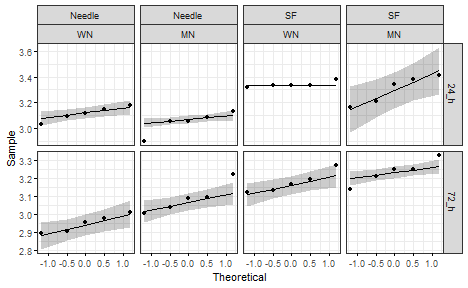
\includegraphics[width=0.95\linewidth,]{Statistics_report_files/figure-latex/qq-plot-figure-1e-f-myeloid-cells-1} 

}

\caption{Fig.1e-f-1: QQ-plots of myeloid cell counts split into groups by predictor variables}\label{fig:qq-plot-figure-1e-f-myeloid-cells}
\end{figure}

\subparagraph{Neutrophils}\label{neutrophils-2}

In spite of assessment limitations due to small group sizes, We concluded based on Shpiro-Wilks test (Table 29) and QQ-pots (Fig.1e-f-2) that all groups of the dataset were approximately normal distributed.

\begin{longtable}{ccclrrl}
\caption*{
{\large \textbf{Appendix Table 29}} \\ 
{\small \textbf{Neutrophils: Univariate Shapito-Wilks test results}}
} \\ 
\toprule
Diet & Route & Time\_point & variable & statistic & p & Outcome \\ 
\midrule\addlinespace[2.5pt]
WN & Needle & 24\_h & Counts & 0.9664 & 0.8514 & ns \\ 
WN & Needle & 72\_h & Counts & 0.9196 & 0.5271 & ns \\ 
MN & Needle & 24\_h & Counts & 0.9650 & 0.8420 & ns \\ 
MN & Needle & 72\_h & Counts & 0.8507 & 0.1967 & ns \\ 
WN & SF & 24\_h & Counts & 0.9704 & 0.8776 & ns \\ 
WN & SF & 72\_h & Counts & 0.9251 & 0.5632 & ns \\ 
MN & SF & 24\_h & Counts & 0.9265 & 0.5725 & ns \\ 
MN & SF & 72\_h & Counts & 0.9361 & 0.6383 & ns \\ 
\bottomrule
\end{longtable}

\begin{figure}[H]

{\centering 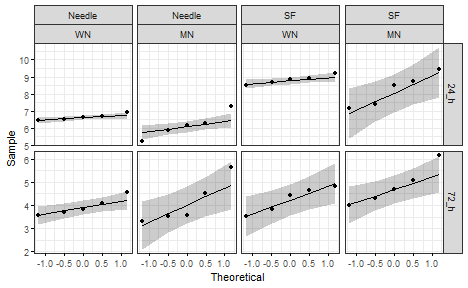
\includegraphics[width=0.95\linewidth,]{Statistics_report_files/figure-latex/qq-plot-figure-1e-f-neutrophils-1} 

}

\caption{Fig.1e-f-2: QQ-plots of neutrophil counts split into groups by predictor variables}\label{fig:qq-plot-figure-1e-f-neutrophils}
\end{figure}

\subparagraph{Monocytes}\label{monocytes-2}

In spite of assessment limitations due to small group sizes, We concluded based on Shpiro-Wilks test (Table 30) and QQ-pots (Fig.1e-f-3) that all groups of the myeloid cell dataset were approximately normal distributed.

\begin{longtable}{ccclrrl}
\caption*{
{\large \textbf{Appendix Table 30}} \\ 
{\small \textbf{Monocytes: Univariate Shapito-Wilks test results}}
} \\ 
\toprule
Diet & Route & Time\_point & variable & statistic & p & Outcome \\ 
\midrule\addlinespace[2.5pt]
WN & Needle & 24\_h & Counts & 0.9542 & 0.7674 & ns \\ 
WN & Needle & 72\_h & Counts & 0.8933 & 0.3740 & ns \\ 
MN & Needle & 24\_h & Counts & 0.9561 & 0.7806 & ns \\ 
MN & Needle & 72\_h & Counts & 0.8828 & 0.3221 & ns \\ 
WN & SF & 24\_h & Counts & 0.8563 & 0.2151 & ns \\ 
WN & SF & 72\_h & Counts & 0.9219 & 0.5422 & ns \\ 
MN & SF & 24\_h & Counts & 0.9430 & 0.6874 & ns \\ 
MN & SF & 72\_h & Counts & 0.8849 & 0.3319 & ns \\ 
\bottomrule
\end{longtable}

\begin{figure}[H]

{\centering 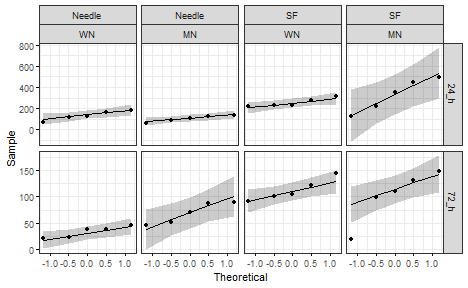
\includegraphics[width=0.95\linewidth,]{Statistics_report_files/figure-latex/qq-plot-figure-1e-f-monocytes-1} 

}

\caption{Fig.1e-f-3: QQ-plots of monocyte counts split into groups by predictor variables}\label{fig:qq-plot-figure-1e-f-monocytes}
\end{figure}

\paragraph{Homogeneity of variance}\label{homogeneity-of-variance-1}

The assessment of homogeneity of variance was also conducted for myeloid cell, neutrophil and monocyte counts separately. We employed a Levene's test for the whole model for each dataset. The p-value for the test suggested that the assumption of homogeneity of variance held for Myeloid\_cells (p=0.5389), held for Neutrophils (p=0.401), and was rejected for Monocytes (p=0.0011).

\paragraph{Outliers}\label{outliers-1}

It can be difficult to determine outliers in small datasets reliably as the analysis is dependent on the interquartile range of the data per group. We attempted it anyway, but increased the coefficient from 1.5 to 3 for less stringency. We found 6 outliers in the Myeloid\_cells dataset (Table 31), 2 outliers in the Neutrophils dataset (Table 32), and 1 outliers in the Monocytes dataset (Table 33).

\begin{longtable}{ccccc}
\caption*{
{\large \textbf{Appendix Table 31}} \\ 
{\small \textbf{Myeloid cells: List of possible outliers}}
} \\ 
\toprule
Diet & Route & Time\_point & is.outlier & is.extreme \\ 
\midrule\addlinespace[2.5pt]
MN & Needle & 24\_h & TRUE & TRUE \\ 
MN & Needle & 72\_h & TRUE & FALSE \\ 
WN & SF & 24\_h & TRUE & TRUE \\ 
WN & SF & 24\_h & TRUE & TRUE \\ 
MN & SF & 72\_h & TRUE & FALSE \\ 
MN & SF & 72\_h & TRUE & FALSE \\ 
\bottomrule
\end{longtable}

\begin{longtable}{ccccc}
\caption*{
{\large \textbf{Appendix Table 32}} \\ 
{\small \textbf{Neutrophils: List of possible outliers}}
} \\ 
\toprule
Diet & Route & Time\_point & is.outlier & is.extreme \\ 
\midrule\addlinespace[2.5pt]
MN & Needle & 24\_h & TRUE & FALSE \\ 
MN & Needle & 24\_h & TRUE & FALSE \\ 
\bottomrule
\end{longtable}

\begin{longtable}{ccccc}
\caption*{
{\large \textbf{Appendix Table 33}} \\ 
{\small \textbf{Monocytes: List of possible outliers}}
} \\ 
\toprule
Diet & Route & Time\_point & is.outlier & is.extreme \\ 
\midrule\addlinespace[2.5pt]
MN & SF & 72\_h & TRUE & FALSE \\ 
\bottomrule
\end{longtable}

\subsubsection{Three-way analysis}\label{three-way-analysis-1}

\paragraph{Myeloid\_cells}\label{myeloid_cells-3}

Based on the assumption analysis, we decided to apply a Simple linear regression to the Myeloid\_cells dataset to determine the effects of ``Diet'', infection ``Route'' and time post infection (``Time\_point'') on the Myeloid\_cells counts per pooled ear single-cell suspension (Table 34). The appropriateness of the Simple linear regression was confirmed by checking the model residuals for normal distribution (Shapiro-Wilks test: 0.771; Fig.1e-f-4).

\begin{figure}[H]

{\centering 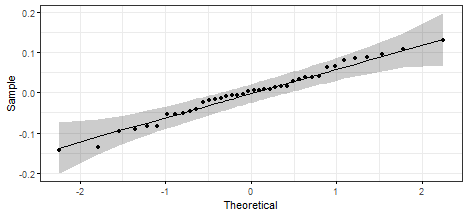
\includegraphics[width=0.95\linewidth,]{Statistics_report_files/figure-latex/qq-plot-figure-1e-f-myeloid-cell-residuals-1} 

}

\caption{Fig.1e-f-4: QQ-plots of monocyte counts split into groups by predictor variables}\label{fig:qq-plot-figure-1e-f-myeloid-cell-residuals}
\end{figure}

The test output of the Simple linear regression showed that only the ``Route'' and ``Time\_point'' predictors were statistically significant factors, while the interaction between Time\_point and Diet was statistically significant, too. The importance of the ``Time\_point'' predictor was a significant difference for the IL1B\textsuperscript{+} Myeloid\_cells counts, compared to observations in figure 1b \& c, when IL1B\textsuperscript{+} was not considered.

\begin{longtable}{l|rrrrlc}
\caption*{
{\large \textbf{Appendix Table 34}} \\ 
{\small \textbf{Myeloid cells: Robust three-way ANOVA}}
} \\ 
\toprule
\multicolumn{1}{l}{Predictors} & Df & Sum Sq & Mean Sq & F value & Pr(>F) & sig. \\ 
\midrule\addlinespace[2.5pt]
Diet & 1 & 0.0056 & 0.0056 & 1.1286 & 0.2960 & ns \\ 
Route & 1 & 0.4567 & 0.4567 & 91.9654 & <0.0001 & **** \\ 
Time\_point & 1 & 0.0750 & 0.0750 & 15.1095 & 0.0005 & *** \\ 
Diet:Route & 1 & 0.0016 & 0.0016 & 0.3309 & 0.5692 & ns \\ 
Diet:Time\_point & 1 & 0.0585 & 0.0585 & 11.7781 & 0.0017 & ** \\ 
Route:Time\_point & 1 & 0.0069 & 0.0069 & 1.3874 & 0.2475 & ns \\ 
Diet:Route:Time\_point & 1 & 0.0080 & 0.0080 & 1.6065 & 0.2141 & ns \\ 
\bottomrule
\end{longtable}

As we performed a Simple linear regression, we were not able to analyze main and simple simple effects of predictors, but moved immediately to perform a pairwise comparison. We applied a Estimated marginal means analysis and the output showed that at 24 h post infection, the sand fly infection route was statistically significant from the control and needle inoculum in the well-nourished (WN) group (Table 37). At 72 h, the sand fly infection route was statistically significant from the control in the malnourished group. Further, statistically significant difference were observed between well-nourished and malnourished mice inoculated by needle at 24 h post infection and infected by sand fly at 72 h post infection.

\begin{longtable}{l|rrrrlc}
\caption*{
{\large \textbf{Appendix Table 37}} \\ 
{\small \textbf{Myeloid cells: Pairwise comparison by Estimated marginal means analysis}}
} \\ 
\toprule
\multicolumn{1}{l}{Pairing} & estimate & SE & df & t.ratio & p.value & sig. \\ 
\midrule\addlinespace[2.5pt]
WN Needle 24\_h - MN Needle 24\_h & 0.0682 & 0.0446 & 32 & 1.5309 & 0.9831 & ns \\ 
WN Needle 24\_h - WN SF 24\_h & -0.2245 & 0.0446 & 32 & -5.0377 & 0.0005 & *** \\ 
WN Needle 24\_h - MN SF 24\_h & -0.1871 & 0.0446 & 32 & -4.1991 & 0.0056 & ** \\ 
WN Needle 24\_h - WN Needle 72\_h & 0.1651 & 0.0446 & 32 & 3.7043 & 0.0221 & * \\ 
WN Needle 24\_h - MN Needle 72\_h & 0.0239 & 0.0446 & 32 & 0.5358 & 1.0000 & ns \\ 
WN Needle 24\_h - WN SF 72\_h & -0.0634 & 0.0446 & 32 & -1.4230 & 0.9935 & ns \\ 
WN Needle 24\_h - MN SF 72\_h & -0.1225 & 0.0446 & 32 & -2.7488 & 0.2399 & ns \\ 
MN Needle 24\_h - WN SF 24\_h & -0.2928 & 0.0446 & 32 & -6.5686 & <0.0001 & **** \\ 
MN Needle 24\_h - MN SF 24\_h & -0.2554 & 0.0446 & 32 & -5.7300 & 0.0001 & **** \\ 
MN Needle 24\_h - WN Needle 72\_h & 0.0969 & 0.0446 & 32 & 2.1734 & 0.6547 & ns \\ 
MN Needle 24\_h - MN Needle 72\_h & -0.0443 & 0.0446 & 32 & -0.9951 & 1.0000 & ns \\ 
MN Needle 24\_h - WN SF 72\_h & -0.1317 & 0.0446 & 32 & -2.9539 & 0.1513 & ns \\ 
MN Needle 24\_h - MN SF 72\_h & -0.1907 & 0.0446 & 32 & -4.2797 & 0.0044 & ** \\ 
WN SF 24\_h - MN SF 24\_h & 0.0374 & 0.0446 & 32 & 0.8386 & 1.0000 & ns \\ 
WN SF 24\_h - WN Needle 72\_h & 0.3896 & 0.0446 & 32 & 8.7421 & <0.0001 & **** \\ 
WN SF 24\_h - MN Needle 72\_h & 0.2484 & 0.0446 & 32 & 5.5735 & 0.0001 & *** \\ 
WN SF 24\_h - WN SF 72\_h & 0.1611 & 0.0446 & 32 & 3.6147 & 0.0282 & * \\ 
WN SF 24\_h - MN SF 72\_h & 0.1020 & 0.0446 & 32 & 2.2889 & 0.5592 & ns \\ 
MN SF 24\_h - WN Needle 72\_h & 0.3522 & 0.0446 & 32 & 7.9034 & <0.0001 & **** \\ 
MN SF 24\_h - MN Needle 72\_h & 0.2110 & 0.0446 & 32 & 4.7349 & 0.0012 & ** \\ 
MN SF 24\_h - WN SF 72\_h & 0.1237 & 0.0446 & 32 & 2.7761 & 0.2262 & ns \\ 
MN SF 24\_h - MN SF 72\_h & 0.0646 & 0.0446 & 32 & 1.4503 & 0.9915 & ns \\ 
WN Needle 72\_h - MN Needle 72\_h & -0.1412 & 0.0446 & 32 & -3.1685 & 0.0900 & + \\ 
WN Needle 72\_h - WN SF 72\_h & -0.2285 & 0.0446 & 32 & -5.1274 & 0.0004 & *** \\ 
WN Needle 72\_h - MN SF 72\_h & -0.2876 & 0.0446 & 32 & -6.4531 & <0.0001 & **** \\ 
MN Needle 72\_h - WN SF 72\_h & -0.0873 & 0.0446 & 32 & -1.9588 & 0.8172 & ns \\ 
MN Needle 72\_h - MN SF 72\_h & -0.1464 & 0.0446 & 32 & -3.2846 & 0.0671 & + \\ 
WN SF 72\_h - MN SF 72\_h & -0.0591 & 0.0446 & 32 & -1.3258 & 0.9976 & ns \\ 
\bottomrule
\end{longtable}

\paragraph{Neutrophils}\label{neutrophils-3}

Based on the assumption analysis, we decided to apply a Robust three-way ANOVA to the Neutrophils dataset to determine the effects of ``Diet'', infection ``Route'' and time post infection (``Time\_point'') on the Neutrophils count per pooled ear single-cell suspension (Table 38). The test output showed that, as for Myeloid\_cells counts, ``Route'' and ``Time\_point'' were both statistically significant predictors, while here, their interaction was also statistically meaningful.

\begin{longtable}{l|rrc}
\caption*{
{\large \textbf{Appendix Table 38}} \\ 
{\small \textbf{Neutrophils: Robust three-way ANOVA}}
} \\ 
\toprule
\multicolumn{1}{l}{Predictors} & value & p.value & sig. \\ 
\midrule\addlinespace[2.5pt]
Diet & 0.6656 & 0.4400 & ns \\ 
Route & 37.4846 & 0.0001 & **** \\ 
Time\_point & 211.6458 & 0.0010 & *** \\ 
Diet:Route & 0.0973 & 0.7640 & ns \\ 
Diet:Time\_point & 2.7393 & 0.1340 & ns \\ 
Route:Time\_point & 11.3037 & 0.0080 & ** \\ 
Diet:Route:Time\_point & 0.3065 & 0.5960 & ns \\ 
\bottomrule
\end{longtable}

We looked for main effects by splitting the data by each predictor separately and analyzed the respective remaining two predictor by a Robust two-way ANOVA. After adjustment of p-values for multiple tests, we observed statistically significant differences for the ``Time\_point'' variable, when the data was split by ``Route'' or by ``Diet''; in well-nourished group for Route, Time\_point and their interaction were statistically meaningful, while for the malnourished state, there was no meaningful interaction between these predictors when the data was split by ``Diet''; and for ``Route was only meaningful at 24 h post infection, when the data was split by Time\_point (Table 39).

\begin{longtable}{l|lrrcrc}
\caption*{
{\large \textbf{Appendix Table 39}} \\ 
{\small \textbf{Neutrophils: Robust two-way ANOVA}}
} \\ 
\toprule
\multicolumn{1}{l}{Grouper} & Predictor & value & p.value & Sig. & p.value.adj & sig. \\ 
\midrule\addlinespace[2.5pt]
\multicolumn{7}{l}{Grouped by Route} \\ 
\midrule\addlinespace[2.5pt]
Needle & Diet &   0.2902 & 0.603 & ns & 0.6784 & ns \\ 
Needle & Time\_point &  68.5031 & 0.001 & *** & 0.0026 & ** \\ 
Needle & Diet:Time\_point &   1.2155 & 0.297 & ns & 0.3819 & ns \\ 
SF & Diet &   0.0001 & 0.993 & ns & 0.9930 & ns \\ 
SF & Time\_point & 159.7806 & 0.001 & *** & 0.0026 & ** \\ 
SF & Diet:Time\_point &   3.4747 & 0.086 & + & 0.1548 & ns \\ 
\midrule\addlinespace[2.5pt]
\multicolumn{7}{l}{Grouped by Diet} \\ 
\midrule\addlinespace[2.5pt]
WN & Route &  55.4130 & 0.001 & *** & 0.0026 & ** \\ 
WN & Time\_point & 479.7172 & 0.001 & *** & 0.0026 & ** \\ 
WN & Route:Time\_point &  31.7623 & 0.001 & *** & 0.0026 & ** \\ 
MN & Route &  12.4507 & 0.003 & ** & 0.0068 & ** \\ 
MN & Time\_point &  48.2204 & 0.001 & *** & 0.0026 & ** \\ 
MN & Route:Time\_point &   2.8633 & 0.110 & ns & 0.1800 & ns \\ 
\midrule\addlinespace[2.5pt]
\multicolumn{7}{l}{Grouped by Time\_point} \\ 
\midrule\addlinespace[2.5pt]
24\_h & Diet &   3.6650 & 0.085 & + & 0.1548 & ns \\ 
24\_h & Route &  57.8683 & 0.001 & *** & 0.0026 & ** \\ 
24\_h & Diet:Route &   0.0452 & 0.837 & ns & 0.8862 & ns \\ 
72\_h & Diet &   1.3260 & 0.272 & ns & 0.3766 & ns \\ 
72\_h & Route &   2.4858 & 0.140 & ns & 0.2100 & ns \\ 
72\_h & Diet:Route &   0.4236 & 0.528 & ns & 0.6336 & ns \\ 
\bottomrule
\end{longtable}

For the analysis of the simple simple main effect for each respective predictor, we performed Robust one-way ANOVA with individual predictors of the data split by the other two predictors. The output showed ``Time\_point'' post infestation was statistically significant across the board, while ``Route'' was only statistically significant during the 24 h time point. ``Diet'' played not significant role as a predictor (Table 40).

\begin{longtable}{lllrrrlrlc}
\caption*{
{\large \textbf{Appendix Table 40}} \\ 
{\small \textbf{Neutrophils: Robust one-way ANOVA}}
} \\ 
\toprule
Predictor\_1 & Predictor\_2 & Effect & test & df1 & df2 & p.value & effsize & p.value.adj & sig. \\ 
\midrule\addlinespace[2.5pt]
\multicolumn{10}{l}{Predictor: Time\_point} \\ 
\midrule\addlinespace[2.5pt]
Needle & WN & Time\_point & 203.3793 & 1 & 5.9585 & <0.0001 & 1.1183 & <0.0001 & **** \\ 
Needle & MN & Time\_point & 14.4271 & 1 & 7.3720 & 0.0061 & 1.0154 & 0.0122 & * \\ 
SF & WN & Time\_point & 280.9801 & 1 & 5.5483 & <0.0001 & 1.1235 & <0.0001 & **** \\ 
SF & MN & Time\_point & 35.7185 & 1 & 7.8502 & 0.0004 & 1.0791 & 0.0011 & ** \\ 
\midrule\addlinespace[2.5pt]
\multicolumn{10}{l}{Predictor: Diet} \\ 
\midrule\addlinespace[2.5pt]
24\_h & Needle & Diet & 1.9911 & 1 & 4.5651 & 0.2226 & 0.7259 & 0.2945 & ns \\ 
24\_h & SF & Diet & 1.7774 & 1 & 4.5402 & 0.2454 & 0.5247 & 0.2945 & ns \\ 
72\_h & Needle & Diet & 0.1201 & 1 & 5.1645 & 0.7426 & 0.2162 & 0.7426 & ns \\ 
72\_h & SF & Diet & 1.6983 & 1 & 6.9708 & 0.2339 & 0.7251 & 0.2945 & ns \\ 
\midrule\addlinespace[2.5pt]
\multicolumn{10}{l}{Predictor: Route} \\ 
\midrule\addlinespace[2.5pt]
24\_h & WN & Route & 236.8953 & 1 & 7.5189 & <0.0001 & 1.1347 & <0.0001 & **** \\ 
24\_h & MN & Route & 14.6124 & 1 & 7.4408 & 0.0058 & 1.0516 & 0.0122 & * \\ 
72\_h & WN & Route & 0.9975 & 1 & 7.0332 & 0.3510 & 0.4008 & 0.3829 & ns \\ 
72\_h & MN & Route & 1.5798 & 1 & 7.8076 & 0.2451 & 0.5136 & 0.2945 & ns \\ 
\bottomrule
\end{longtable}

For the pairwise comparison, we applied a Linear contrast expression. As all three factors where dichotomous, the pairwise comparison reflected the one-way ANVOA results (Table 41).

\begin{longtable}{llccrrrlc}
\caption*{
{\large \textbf{Appendix Table 41}} \\ 
{\small \textbf{Neutrophils: Pairwise comparison by Linear Contrast Expression}}
} \\ 
\toprule
Predictor\_1 & Predictor\_2 & Group & Group.1 & psihat & ci.lower & ci.upper & p.value & Sig. \\ 
\midrule\addlinespace[2.5pt]
\multicolumn{9}{l}{Predictor: Time\_point} \\ 
\midrule\addlinespace[2.5pt]
Needle & WN & 24\_h & 72\_h & 2.7044 & 2.2396 & 3.1692 & <0.0001 & **** \\ 
Needle & MN & 24\_h & 72\_h & 2.0686 & 0.7938 & 3.3433 & 0.0061 & ** \\ 
SF & WN & 24\_h & 72\_h & 4.5783 & 3.8966 & 5.2600 & <0.0001 & **** \\ 
SF & MN & 24\_h & 72\_h & 3.4015 & 2.0847 & 4.7184 & 0.0004 & *** \\ 
\midrule\addlinespace[2.5pt]
\multicolumn{9}{l}{Predictor: Diet} \\ 
\midrule\addlinespace[2.5pt]
24\_h & Needle & WN & MN & 0.4732 & -0.4142 & 1.3606 & 0.2226 & ns \\ 
24\_h & SF & WN & MN & 0.5915 & -0.5846 & 1.7676 & 0.2454 & ns \\ 
72\_h & Needle & WN & MN & -0.1626 & -1.3570 & 1.0319 & 0.7426 & ns \\ 
72\_h & SF & WN & MN & -0.5853 & -1.6481 & 0.4776 & 0.2339 & ns \\ 
\midrule\addlinespace[2.5pt]
\multicolumn{9}{l}{Predictor: Route} \\ 
\midrule\addlinespace[2.5pt]
24\_h & WN & Needle & SF & -2.1745 & -2.5040 & -1.8451 & <0.0001 & **** \\ 
24\_h & MN & Needle & SF & -2.0563 & -3.3131 & -0.7994 & 0.0058 & ** \\ 
72\_h & WN & Needle & SF & -0.3006 & -1.0117 & 0.4104 & 0.3510 & ns \\ 
72\_h & MN & Needle & SF & -0.7233 & -2.0561 & 0.6095 & 0.2451 & ns \\ 
\bottomrule
\end{longtable}

\paragraph{Monocytes}\label{monocytes-3}

Based on the assumption analysis, we decided to apply a Robust three-way ANOVA to the Monocytes dataset to determine the effects of ``Diet'', infection ``Route'' and time post infection (``Time\_point'') on the Monocytes count per pooled ear single-cell suspension (Table 42). As for Myeloid\_cells and Neutrophils counts, ``Route'' and ``Time\_point'' were statistically significant predictors. However, not significant interaction between predictors was observed for Monocytes counts.

\begin{longtable}{l|rrc}
\caption*{
{\large \textbf{Appendix Table 42}} \\ 
{\small \textbf{Monocytes: Robust three-way ANOVA}}
} \\ 
\toprule
\multicolumn{1}{l}{Predictors} & value & p.value & sig. \\ 
\midrule\addlinespace[2.5pt]
Diet & 1.1474 & 0.360 & ns \\ 
Route & 20.1101 & 0.006 & ** \\ 
Time\_point & 24.8237 & 0.003 & ** \\ 
Diet:Route & 0.8115 & 0.428 & ns \\ 
Diet:Time\_point & 0.0604 & 0.822 & ns \\ 
Route:Time\_point & 4.6317 & 0.096 & + \\ 
Diet:Route:Time\_point & 2.4210 & 0.200 & ns \\ 
\bottomrule
\end{longtable}

We looked for main effects by splitting the data by each predictor separately and analyzed the respective remaining two predictor by a Robust two-way ANOVA. After adjustment of p-values for multiple tests, we observed statistically significant differences for the ``Time\_point'' variable, when the data was split by ``Route'' or by ``Diet''; in well-nourished and mal-nourished groups we observed statistical significance for ``Route'' and ``Time\_point'', while no significant interactions were observed when the data was split by ``Diet''; and for ``Route'' was meaningful at both, 24 h and 72 h post infection, when the data was split by Time\_point (Table 43). Overall, ``Diet'' played not meaning role as a predictor.

\begin{longtable}{l|lrrcrc}
\caption*{
{\large \textbf{Appendix Table 43}} \\ 
{\small \textbf{Monovytes: Robust two-way ANOVA}}
} \\ 
\toprule
\multicolumn{1}{l}{Grouper} & Predictor & value & p.value & Sig. & p.value.adj & sig. \\ 
\midrule\addlinespace[2.5pt]
\multicolumn{7}{l}{Grouped by Route} \\ 
\midrule\addlinespace[2.5pt]
Needle & Diet &  0.0991 & 0.760 & ns & 0.7600 & ns \\ 
Needle & Time\_point & 25.6851 & 0.001 & *** & 0.0045 & ** \\ 
Needle & Diet:Time\_point &  5.7556 & 0.034 & * & 0.0680 & + \\ 
SF & Diet &  0.6918 & 0.437 & ns & 0.4916 & ns \\ 
SF & Time\_point & 23.4448 & 0.001 & *** & 0.0045 & ** \\ 
SF & Diet:Time\_point &  1.2852 & 0.298 & ns & 0.3831 & ns \\ 
\midrule\addlinespace[2.5pt]
\multicolumn{7}{l}{Grouped by Diet} \\ 
\midrule\addlinespace[2.5pt]
WN & Route & 47.9950 & 0.001 & *** & 0.0045 & ** \\ 
WN & Time\_point & 68.8826 & 0.001 & *** & 0.0045 & ** \\ 
WN & Route:Time\_point &  1.9584 & 0.189 & ns & 0.2835 & ns \\ 
MN & Route & 11.5996 & 0.010 & ** & 0.0225 & * \\ 
MN & Time\_point & 12.2280 & 0.009 & ** & 0.0225 & * \\ 
MN & Route:Time\_point &  6.4702 & 0.038 & * & 0.0684 & + \\ 
\midrule\addlinespace[2.5pt]
\multicolumn{7}{l}{Grouped by Time\_point} \\ 
\midrule\addlinespace[2.5pt]
24\_h & Diet &  0.3760 & 0.562 & ns & 0.5951 & ns \\ 
24\_h & Route & 20.4756 & 0.002 & ** & 0.0060 & ** \\ 
24\_h & Diet:Route &  1.8171 & 0.223 & ns & 0.3088 & ns \\ 
72\_h & Diet &  0.8951 & 0.373 & ns & 0.4476 & ns \\ 
72\_h & Route & 18.2554 & 0.002 & ** & 0.0060 & ** \\ 
72\_h & Diet:Route &  3.2974 & 0.105 & ns & 0.1718 & ns \\ 
\bottomrule
\end{longtable}

For the analysis of the simple simple main effect for each respective predictor, we performed Robust one-way ANOVA with individual predictors of the data split by the other two predictors. The output showed ``Time\_point'' post infestation was statistically significant across the board with the exception for malnourished individuals inoculated by needle, while ``Route'' was only statistically significant during the within the well-nourished group at either time point. ``Diet'' was only statistically significant for the needle inoculated groups at 72 h post infection (Table 44).

\begin{longtable}{lllrrrrrrc}
\caption*{
{\large \textbf{Appendix Table 44}} \\ 
{\small \textbf{Monocytes: Robust one-way ANOVA}}
} \\ 
\toprule
Predictor\_1 & Predictor\_2 & Effect & test & df1 & df2 & p.value & effsize & p.value.adj & sig. \\ 
\midrule\addlinespace[2.5pt]
\multicolumn{10}{l}{Predictor: Time\_point} \\ 
\midrule\addlinespace[2.5pt]
Needle & WN & Time\_point & 24.2428 & 1 & 4.4410 & 0.0060 & 1.0016 & 0.0181 & * \\ 
Needle & MN & Time\_point & 4.1902 & 1 & 6.5974 & 0.0823 & 0.7082 & 0.1235 & ns \\ 
SF & WN & Time\_point & 46.2024 & 1 & 5.9611 & 0.0005 & 1.1175 & 0.0031 & ** \\ 
SF & MN & Time\_point & 9.6448 & 1 & 4.8214 & 0.0280 & 0.9127 & 0.0528 & + \\ 
\midrule\addlinespace[2.5pt]
\multicolumn{10}{l}{Predictor: Diet} \\ 
\midrule\addlinespace[2.5pt]
24\_h & Needle & Diet & 1.2696 & 1 & 7.4413 & 0.2949 & 0.4586 & 0.3538 & ns \\ 
24\_h & SF & Diet & 1.0760 & 1 & 4.5597 & 0.3514 & 0.4648 & 0.3834 & ns \\ 
72\_h & Needle & Diet & 12.7301 & 1 & 5.9683 & 0.0119 & 0.8820 & 0.0286 & * \\ 
72\_h & SF & Diet & 0.2225 & 1 & 5.3766 & 0.6557 & 0.3242 & 0.6557 & ns \\ 
\midrule\addlinespace[2.5pt]
\multicolumn{10}{l}{Predictor: Route} \\ 
\midrule\addlinespace[2.5pt]
24\_h & WN & Route & 19.9581 & 1 & 7.9596 & 0.0021 & 1.1520 & 0.0085 & ** \\ 
24\_h & MN & Route & 9.8710 & 1 & 4.3690 & 0.0308 & 0.8864 & 0.0528 & + \\ 
72\_h & WN & Route & 58.1556 & 1 & 5.8388 & 0.0003 & 1.1400 & 0.0031 & ** \\ 
72\_h & MN & Route & 1.7950 & 1 & 5.2796 & 0.2351 & 0.5765 & 0.3135 & ns \\ 
\bottomrule
\end{longtable}

For the pairwise comparison, we applied a Linear contrast expression. As all three factors where dichotomous, the pairwise comparison reflected the one-way ANVOA results (Table 45).

\begin{longtable}{llccrrrrc}
\caption*{
{\large \textbf{Appendix Table 45}} \\ 
{\small \textbf{Monocytes: Pairwise comparison by Linear Contrast Expression}}
} \\ 
\toprule
Predictor\_1 & Predictor\_2 & Group & Group.1 & psihat & ci.lower & ci.upper & p.value & Sig. \\ 
\midrule\addlinespace[2.5pt]
\multicolumn{9}{l}{Predictor: Time\_point} \\ 
\midrule\addlinespace[2.5pt]
Needle & WN & 24\_h & 72\_h & 99.6 & 45.5687 & 153.6313 & 0.0060 & ** \\ 
Needle & MN & 24\_h & 72\_h & 35.6 & -6.0383 & 77.2383 & 0.0823 & + \\ 
SF & WN & 24\_h & 72\_h & 140.0 & 89.5221 & 190.4779 & 0.0005 & *** \\ 
SF & MN & 24\_h & 72\_h & 225.6 & 36.7654 & 414.4346 & 0.0280 & * \\ 
\midrule\addlinespace[2.5pt]
\multicolumn{9}{l}{Predictor: Diet} \\ 
\midrule\addlinespace[2.5pt]
24\_h & Needle & WN & MN & 27.8 & -29.8466 & 85.4466 & 0.2949 & ns \\ 
24\_h & SF & WN & MN & -74.2 & -263.5526 & 115.1526 & 0.3514 & ns \\ 
72\_h & Needle & WN & MN & -36.2 & -61.0582 & -11.3418 & 0.0119 & * \\ 
72\_h & SF & WN & MN & 11.4 & -49.4453 & 72.2453 & 0.6557 & ns \\ 
\midrule\addlinespace[2.5pt]
\multicolumn{9}{l}{Predictor: Route} \\ 
\midrule\addlinespace[2.5pt]
24\_h & WN & Needle & SF & -120.2 & -182.2997 & -58.1003 & 0.0021 & ** \\ 
24\_h & MN & Needle & SF & -222.2 & -412.1896 & -32.2104 & 0.0308 & * \\ 
72\_h & WN & Needle & SF & -79.8 & -105.5774 & -54.0226 & 0.0003 & *** \\ 
72\_h & MN & Needle & SF & -32.2 & -93.0104 & 28.6104 & 0.2351 & ns \\ 
\bottomrule
\end{longtable}

\subsubsection{Statistical power}\label{statistical-power-1}

Considering the small group \emph{N}=5, it stood to reason that the study design was statistically underpowered by necessity to keep animal number and costs manageable. Thus, we performed a retrospective power analysis on the data by cell-type group to explore this.

\paragraph{\texorpdfstring{Effect size estimation based on partial eta\textsuperscript{2}}{Effect size estimation based on partial eta2}}\label{effect-size-estimation-based-on-partial-eta2-1}

Effect sizes were calculated by predictor and the different potential interaction combinations of them. Appendix tables 46 to 48 show the respective effect sizes. Note that upper ends of the confidence intervals were automatically set to 1 for this type of calculation. Large effect sizes reflected statistically meaningful differences in the data analysis. The partial eta\textsuperscript{2} values from the effect size calculation were then used to the retrospective power calculations.

\begin{longtable}{lrrrcl}
\caption*{
{\large \textbf{Appendix Table 46}} \\ 
{\small \textbf{Myeloid cells: Effect size estimation}}
} \\ 
\toprule
Parameter & Eta2\_partial & CI\_low & CI\_high & Effect\_size & Effect Size \\ 
\midrule\addlinespace[2.5pt]
Diet & 0.0125 & 0.0000 & 1 & very small & small \\ 
Route & 0.6490 & 0.4742 & 1 & large & large \\ 
Time\_point & 0.3162 & 0.1108 & 1 & large & large \\ 
Diet:Route & 0.0001 & 0.0000 & 1 & very small & very small \\ 
Diet:Time\_point & 0.0965 & 0.0000 & 1 & small & medium \\ 
Route:Time\_point & 0.2078 & 0.0382 & 1 & medium & large \\ 
Diet:Route:Time\_point & 0.0001 & 0.0000 & 1 & very small & very small \\ 
\bottomrule
\end{longtable}

\begin{longtable}{lrrrcl}
\caption*{
{\large \textbf{Appendix Table 47}} \\ 
{\small \textbf{Neutrophils: Effect size estimation}}
} \\ 
\toprule
Parameter & Eta2\_partial & CI\_low & CI\_high & Effect\_size & Effect Size \\ 
\midrule\addlinespace[2.5pt]
Diet & 0.0330 & 0.0000 & 1 & small & small \\ 
Route & 0.5814 & 0.3864 & 1 & large & large \\ 
Time\_point & 0.7717 & 0.6469 & 1 & large & large \\ 
Diet:Route & 0.0117 & 0.0000 & 1 & very small & small \\ 
Diet:Time\_point & 0.0758 & 0.0000 & 1 & small & medium \\ 
Route:Time\_point & 0.5408 & 0.3368 & 1 & large & large \\ 
Diet:Route:Time\_point & 0.0223 & 0.0000 & 1 & small & small \\ 
\bottomrule
\end{longtable}

\begin{longtable}{lrrrcl}
\caption*{
{\large \textbf{Appendix Table 48}} \\ 
{\small \textbf{Monocytes: Effect size estimation}}
} \\ 
\toprule
Parameter & Eta2\_partial & CI\_low & CI\_high & Effect\_size & Effect Size \\ 
\midrule\addlinespace[2.5pt]
Diet & 0.0241 & 0.0000 & 1 & small & small \\ 
Route & 0.5015 & 0.2911 & 1 & large & large \\ 
Time\_point & 0.5500 & 0.3478 & 1 & large & large \\ 
Diet:Route & 0.0142 & 0.0000 & 1 & very small & small \\ 
Diet:Time\_point & 0.0023 & 0.0000 & 1 & very small & very small \\ 
Route:Time\_point & 0.2055 & 0.0370 & 1 & medium & large \\ 
Diet:Route:Time\_point & 0.0983 & 0.0000 & 1 & small & medium \\ 
\bottomrule
\end{longtable}

\paragraph{Retrospective minimum total sample size estimation for 80\% power}\label{retrospective-minimum-total-sample-size-estimation-for-80-power-1}

The accepted rule of thumb is to have at least 80\% (0.8 as ratio) statistical power in once data. For small mean differences within data of a high level of complexity, this is often hard to achieve, because of cost and ability to manage large sample sizes. For Myeloid\_cells, the predictors ``Route'' and ``Time\_point'' as much as the interaction ``Diet:Time\_point'' resulted in optimal sample sizes that were within the total sample size of \emph{N}=40, 40, 40 (Appendix table 49). The large proposed sample sizes for ``Diet'' on its own and within most of its interactions suggested little statistically significant difference between groups with respect to ``Diet''.

\begin{longtable}{l|rrrrr}
\caption*{
{\large \textbf{Appendix Table 49}} \\ 
{\small \textbf{Myeloid Cells: Minimum optimal sample size calculation}}
} \\ 
\toprule
\multicolumn{1}{l}{Effect} & power & n.total & ncp & df1 & df2 \\ 
\midrule\addlinespace[2.5pt]
\multicolumn{6}{l}{Diet} \\ 
\midrule\addlinespace[2.5pt]
Diet & 0.8 & 620 & 7.873 & 1 & 617.5 \\ 
\midrule\addlinespace[2.5pt]
\multicolumn{6}{l}{Route} \\ 
\midrule\addlinespace[2.5pt]
Route & 0.8 & 7 & 12.601 & 1 & 4.815 \\ 
\midrule\addlinespace[2.5pt]
\multicolumn{6}{l}{Time\_point} \\ 
\midrule\addlinespace[2.5pt]
Time\_point & 0.8 & 20 & 8.832 & 1 & 17.095 \\ 
\midrule\addlinespace[2.5pt]
\multicolumn{6}{l}{Diet:Route} \\ 
\midrule\addlinespace[2.5pt]
Diet & 0.8 & 64408 & 7.849 & 1 & 64403.09 \\ 
Route & 0.8 & 64408 & 7.849 & 1 & 64403.09 \\ 
Diet:Route & 0.8 & 64408 & 7.849 & 1 & 64403.09 \\ 
\midrule\addlinespace[2.5pt]
\multicolumn{6}{l}{Diet:Time\_point} \\ 
\midrule\addlinespace[2.5pt]
Diet & 0.8 & 76 & 8.065 & 1 & 71.503 \\ 
Time\_point & 0.8 & 76 & 8.065 & 1 & 71.503 \\ 
Diet:Time\_point & 0.8 & 76 & 8.065 & 1 & 71.503 \\ 
\midrule\addlinespace[2.5pt]
\multicolumn{6}{l}{Route:Time\_point} \\ 
\midrule\addlinespace[2.5pt]
Route & 0.8 & 33 & 8.422 & 1 & 28.106 \\ 
Time\_point & 0.8 & 33 & 8.422 & 1 & 28.106 \\ 
Route:Time\_point & 0.8 & 33 & 8.422 & 1 & 28.106 \\ 
\midrule\addlinespace[2.5pt]
\multicolumn{6}{l}{Diet:Route:Time\_point} \\ 
\midrule\addlinespace[2.5pt]
Diet & 0.8 & 83400 & 7.849 & 1 & 83391.34 \\ 
Route & 0.8 & 83400 & 7.849 & 1 & 83391.34 \\ 
Time\_point & 0.8 & 83400 & 7.849 & 1 & 83391.34 \\ 
Diet:Route & 0.8 & 83400 & 7.849 & 1 & 83391.34 \\ 
Diet:Time\_point & 0.8 & 83400 & 7.849 & 1 & 83391.34 \\ 
Route:Time\_point & 0.8 & 83400 & 7.849 & 1 & 83391.34 \\ 
Diet:Route:Time\_point & 0.8 & 83400 & 7.849 & 1 & 83391.34 \\ 
\bottomrule
\end{longtable}

Similar observation were made for Neutrophils counts, but here the interaction ``Route:Time\_point'' was within the total sample size of \emph{N}=40, 40, 40 (Appendix Table 50). The involvement of ``Diet'' produced large minimum sample sizes again, suggesting that no true difference may be observed here with respect to ``Diet''.

\begin{longtable}{l|rrrrr}
\caption*{
{\large \textbf{Appendix Table 50}} \\ 
{\small \textbf{Neutrophils: Minimum optimal sample size calculation}}
} \\ 
\toprule
\multicolumn{1}{l}{Effect} & power & n.total & ncp & df1 & df2 \\ 
\midrule\addlinespace[2.5pt]
\multicolumn{6}{l}{Diet} \\ 
\midrule\addlinespace[2.5pt]
Diet & 0.8 & 232 & 7.915 & 1 & 229.662 \\ 
\midrule\addlinespace[2.5pt]
\multicolumn{6}{l}{Route} \\ 
\midrule\addlinespace[2.5pt]
Route & 0.8 & 9 & 11.256 & 1 & 6.104 \\ 
\midrule\addlinespace[2.5pt]
\multicolumn{6}{l}{Time\_point} \\ 
\midrule\addlinespace[2.5pt]
Time\_point & 0.8 & 6 & 17.344 & 1 & 3.132 \\ 
\midrule\addlinespace[2.5pt]
\multicolumn{6}{l}{Diet:Route} \\ 
\midrule\addlinespace[2.5pt]
Diet & 0.8 & 665 & 7.872 & 1 & 660.599 \\ 
Route & 0.8 & 665 & 7.872 & 1 & 660.599 \\ 
Diet:Route & 0.8 & 665 & 7.872 & 1 & 660.599 \\ 
\midrule\addlinespace[2.5pt]
\multicolumn{6}{l}{Diet:Time\_point} \\ 
\midrule\addlinespace[2.5pt]
Diet & 0.8 & 98 & 8.013 & 1 & 93.677 \\ 
Time\_point & 0.8 & 98 & 8.013 & 1 & 93.677 \\ 
Diet:Time\_point & 0.8 & 98 & 8.013 & 1 & 93.677 \\ 
\midrule\addlinespace[2.5pt]
\multicolumn{6}{l}{Route:Time\_point} \\ 
\midrule\addlinespace[2.5pt]
Route & 0.8 & 10 & 11.518 & 1 & 5.78 \\ 
Time\_point & 0.8 & 10 & 11.518 & 1 & 5.78 \\ 
Route:Time\_point & 0.8 & 10 & 11.518 & 1 & 5.78 \\ 
\midrule\addlinespace[2.5pt]
\multicolumn{6}{l}{Diet:Route:Time\_point} \\ 
\midrule\addlinespace[2.5pt]
Diet & 0.8 & 347 & 7.894 & 1 & 338.278 \\ 
Route & 0.8 & 347 & 7.894 & 1 & 338.278 \\ 
Time\_point & 0.8 & 347 & 7.894 & 1 & 338.278 \\ 
Diet:Route & 0.8 & 347 & 7.894 & 1 & 338.278 \\ 
Diet:Time\_point & 0.8 & 347 & 7.894 & 1 & 338.278 \\ 
Route:Time\_point & 0.8 & 347 & 7.894 & 1 & 338.278 \\ 
Diet:Route:Time\_point & 0.8 & 347 & 7.894 & 1 & 338.278 \\ 
\bottomrule
\end{longtable}

For Monocytes counts, the same observations were true as for Myeloid\_cells counts with the exception that ``Diet'' did not have a major detrimental effect on predicted minimum sample size for the three way interaction (``Diet:Route:Time\_point''; Appendix Table 51).

\begin{longtable}{l|rrrrr}
\caption*{
{\large \textbf{Appendix Table 51}} \\ 
{\small \textbf{Monocytes: Minimum optimal sample size calculation}}
} \\ 
\toprule
\multicolumn{1}{l}{Effect} & power & n.total & ncp & df1 & df2 \\ 
\midrule\addlinespace[2.5pt]
\multicolumn{6}{l}{Diet} \\ 
\midrule\addlinespace[2.5pt]
Diet & 0.8 & 320 & 7.897 & 1 & 317.655 \\ 
\midrule\addlinespace[2.5pt]
\multicolumn{6}{l}{Route} \\ 
\midrule\addlinespace[2.5pt]
Route & 0.8 & 11 & 10.197 & 1 & 8.134 \\ 
\midrule\addlinespace[2.5pt]
\multicolumn{6}{l}{Time\_point} \\ 
\midrule\addlinespace[2.5pt]
Time\_point & 0.8 & 9 & 10.786 & 1 & 6.826 \\ 
\midrule\addlinespace[2.5pt]
\multicolumn{6}{l}{Diet:Route} \\ 
\midrule\addlinespace[2.5pt]
Diet & 0.8 & 547 & 7.877 & 1 & 542.2 \\ 
Route & 0.8 & 547 & 7.877 & 1 & 542.2 \\ 
Diet:Route & 0.8 & 547 & 7.877 & 1 & 542.2 \\ 
\midrule\addlinespace[2.5pt]
\multicolumn{6}{l}{Diet:Time\_point} \\ 
\midrule\addlinespace[2.5pt]
Diet & 0.8 & 3455 & 7.853 & 1 & 3450.162 \\ 
Time\_point & 0.8 & 3455 & 7.853 & 1 & 3450.162 \\ 
Diet:Time\_point & 0.8 & 3455 & 7.853 & 1 & 3450.162 \\ 
\midrule\addlinespace[2.5pt]
\multicolumn{6}{l}{Route:Time\_point} \\ 
\midrule\addlinespace[2.5pt]
Route & 0.8 & 33 & 8.413 & 1 & 28.521 \\ 
Time\_point & 0.8 & 33 & 8.413 & 1 & 28.521 \\ 
Route:Time\_point & 0.8 & 33 & 8.413 & 1 & 28.521 \\ 
\midrule\addlinespace[2.5pt]
\multicolumn{6}{l}{Diet:Route:Time\_point} \\ 
\midrule\addlinespace[2.5pt]
Diet & 0.8 & 75 & 8.083 & 1 & 66.118 \\ 
Route & 0.8 & 75 & 8.083 & 1 & 66.118 \\ 
Time\_point & 0.8 & 75 & 8.083 & 1 & 66.118 \\ 
Diet:Route & 0.8 & 75 & 8.083 & 1 & 66.118 \\ 
Diet:Time\_point & 0.8 & 75 & 8.083 & 1 & 66.118 \\ 
Route:Time\_point & 0.8 & 75 & 8.083 & 1 & 66.118 \\ 
Diet:Route:Time\_point & 0.8 & 75 & 8.083 & 1 & 66.118 \\ 
\bottomrule
\end{longtable}

\paragraph{Retrospective calculation of statistical power in our data analysis}\label{retrospective-calculation-of-statistical-power-in-our-data-analysis-1}

The observations from the retrospective minimum sample size calculation was reflected in the power calculation for our data. For Myeloid\_cells counts, only ``Route'' and ``Time\_point'' and the interaction of ``Diet:Time\_point'' had sufficient statistical power to have a change to find statistically meaning differences in the data (Appendix Table 52).

\begin{longtable}{l|rrrrr}
\caption*{
{\large \textbf{Appendix Table 52}} \\ 
{\small \textbf{Myeloid Cells: Statistical power of data}}
} \\ 
\toprule
\multicolumn{1}{l}{Effect} & power & n.total & ncp & df1 & df2 \\ 
\midrule\addlinespace[2.5pt]
\multicolumn{6}{l}{Diet} \\ 
\midrule\addlinespace[2.5pt]
Diet & 0.107 & 40 & 0.508 & 1 & 38 \\ 
\midrule\addlinespace[2.5pt]
\multicolumn{6}{l}{Route} \\ 
\midrule\addlinespace[2.5pt]
Route & 1 & 40 & 73.967 & 1 & 38 \\ 
\midrule\addlinespace[2.5pt]
\multicolumn{6}{l}{Time\_point} \\ 
\midrule\addlinespace[2.5pt]
Time\_point & 0.987 & 40 & 18.501 & 1 & 38 \\ 
\midrule\addlinespace[2.5pt]
\multicolumn{6}{l}{Diet:Route} \\ 
\midrule\addlinespace[2.5pt]
Diet & 0.051 & 40 & 0.005 & 1 & 36 \\ 
Route & 0.051 & 40 & 0.005 & 1 & 36 \\ 
Diet:Route & 0.051 & 40 & 0.005 & 1 & 36 \\ 
\midrule\addlinespace[2.5pt]
\multicolumn{6}{l}{Diet:Time\_point} \\ 
\midrule\addlinespace[2.5pt]
Diet & 0.521 & 40 & 4.273 & 1 & 36 \\ 
Time\_point & 0.521 & 40 & 4.273 & 1 & 36 \\ 
Diet:Time\_point & 0.521 & 40 & 4.273 & 1 & 36 \\ 
\midrule\addlinespace[2.5pt]
\multicolumn{6}{l}{Route:Time\_point} \\ 
\midrule\addlinespace[2.5pt]
Route & 0.883 & 40 & 10.492 & 1 & 36 \\ 
Time\_point & 0.883 & 40 & 10.492 & 1 & 36 \\ 
Route:Time\_point & 0.883 & 40 & 10.492 & 1 & 36 \\ 
\midrule\addlinespace[2.5pt]
\multicolumn{6}{l}{Diet:Route:Time\_point} \\ 
\midrule\addlinespace[2.5pt]
Diet & 0.05 & 40 & 0.004 & 1 & 32 \\ 
Route & 0.05 & 40 & 0.004 & 1 & 32 \\ 
Time\_point & 0.05 & 40 & 0.004 & 1 & 32 \\ 
Diet:Route & 0.05 & 40 & 0.004 & 1 & 32 \\ 
Diet:Time\_point & 0.05 & 40 & 0.004 & 1 & 32 \\ 
Route:Time\_point & 0.05 & 40 & 0.004 & 1 & 32 \\ 
Diet:Route:Time\_point & 0.05 & 40 & 0.004 & 1 & 32 \\ 
\bottomrule
\end{longtable}

For Neutrophils counts, ``Route'' and ``Time\_points as much as their interaction had \textgreater80\% statistical power, while the interaction''Diet:Time\_point'' was close to 80\% statistical power (Appendix Table 53).

\begin{longtable}{l|rrrrr}
\caption*{
{\large \textbf{Appendix Table 53}} \\ 
{\small \textbf{Neutrophils: Statistical power of data}}
} \\ 
\toprule
\multicolumn{1}{l}{Effect} & power & n.total & ncp & df1 & df2 \\ 
\midrule\addlinespace[2.5pt]
\multicolumn{6}{l}{Diet} \\ 
\midrule\addlinespace[2.5pt]
Diet & 0.207 & 40 & 1.367 & 1 & 38 \\ 
\midrule\addlinespace[2.5pt]
\multicolumn{6}{l}{Route} \\ 
\midrule\addlinespace[2.5pt]
Route & 1 & 40 & 55.554 & 1 & 38 \\ 
\midrule\addlinespace[2.5pt]
\multicolumn{6}{l}{Time\_point} \\ 
\midrule\addlinespace[2.5pt]
Time\_point & 1 & 40 & 135.188 & 1 & 38 \\ 
\midrule\addlinespace[2.5pt]
\multicolumn{6}{l}{Diet:Route} \\ 
\midrule\addlinespace[2.5pt]
Diet & 0.103 & 40 & 0.474 & 1 & 36 \\ 
Route & 0.103 & 40 & 0.474 & 1 & 36 \\ 
Diet:Route & 0.103 & 40 & 0.474 & 1 & 36 \\ 
\midrule\addlinespace[2.5pt]
\multicolumn{6}{l}{Diet:Time\_point} \\ 
\midrule\addlinespace[2.5pt]
Diet & 0.422 & 40 & 3.281 & 1 & 36 \\ 
Time\_point & 0.422 & 40 & 3.281 & 1 & 36 \\ 
Diet:Time\_point & 0.422 & 40 & 3.281 & 1 & 36 \\ 
\midrule\addlinespace[2.5pt]
\multicolumn{6}{l}{Route:Time\_point} \\ 
\midrule\addlinespace[2.5pt]
Route & 1 & 40 & 47.107 & 1 & 36 \\ 
Time\_point & 1 & 40 & 47.107 & 1 & 36 \\ 
Route:Time\_point & 1 & 40 & 47.107 & 1 & 36 \\ 
\midrule\addlinespace[2.5pt]
\multicolumn{6}{l}{Diet:Route:Time\_point} \\ 
\midrule\addlinespace[2.5pt]
Diet & 0.153 & 40 & 0.912 & 1 & 32 \\ 
Route & 0.153 & 40 & 0.912 & 1 & 32 \\ 
Time\_point & 0.153 & 40 & 0.912 & 1 & 32 \\ 
Diet:Route & 0.153 & 40 & 0.912 & 1 & 32 \\ 
Diet:Time\_point & 0.153 & 40 & 0.912 & 1 & 32 \\ 
Route:Time\_point & 0.153 & 40 & 0.912 & 1 & 32 \\ 
Diet:Route:Time\_point & 0.153 & 40 & 0.912 & 1 & 32 \\ 
\bottomrule
\end{longtable}

Similar to Neutrophils counts, for Monocytes counts, ``Route'' and ``Time\_points as much as their interaction had \textgreater80\% statistical power, while the interaction''Diet:Time\_point'' was close to 80\% statistical power (Appendix Table 54).

\begin{longtable}{l|rrrrr}
\caption*{
{\large \textbf{Appendix Table 54}} \\ 
{\small \textbf{Monocytes: Statistical power of data}}
} \\ 
\toprule
\multicolumn{1}{l}{Effect} & power & n.total & ncp & df1 & df2 \\ 
\midrule\addlinespace[2.5pt]
\multicolumn{6}{l}{Diet} \\ 
\midrule\addlinespace[2.5pt]
Diet & 0.163 & 40 & 0.988 & 1 & 38 \\ 
\midrule\addlinespace[2.5pt]
\multicolumn{6}{l}{Route} \\ 
\midrule\addlinespace[2.5pt]
Route & 1 & 40 & 40.247 & 1 & 38 \\ 
\midrule\addlinespace[2.5pt]
\multicolumn{6}{l}{Time\_point} \\ 
\midrule\addlinespace[2.5pt]
Time\_point & 1 & 40 & 48.886 & 1 & 38 \\ 
\midrule\addlinespace[2.5pt]
\multicolumn{6}{l}{Diet:Route} \\ 
\midrule\addlinespace[2.5pt]
Diet & 0.115 & 40 & 0.577 & 1 & 36 \\ 
Route & 0.115 & 40 & 0.577 & 1 & 36 \\ 
Diet:Route & 0.115 & 40 & 0.577 & 1 & 36 \\ 
\midrule\addlinespace[2.5pt]
\multicolumn{6}{l}{Diet:Time\_point} \\ 
\midrule\addlinespace[2.5pt]
Diet & 0.06 & 40 & 0.091 & 1 & 36 \\ 
Time\_point & 0.06 & 40 & 0.091 & 1 & 36 \\ 
Diet:Time\_point & 0.06 & 40 & 0.091 & 1 & 36 \\ 
\midrule\addlinespace[2.5pt]
\multicolumn{6}{l}{Route:Time\_point} \\ 
\midrule\addlinespace[2.5pt]
Route & 0.879 & 40 & 10.347 & 1 & 36 \\ 
Time\_point & 0.879 & 40 & 10.347 & 1 & 36 \\ 
Route:Time\_point & 0.879 & 40 & 10.347 & 1 & 36 \\ 
\midrule\addlinespace[2.5pt]
\multicolumn{6}{l}{Diet:Route:Time\_point} \\ 
\midrule\addlinespace[2.5pt]
Diet & 0.526 & 40 & 4.362 & 1 & 32 \\ 
Route & 0.526 & 40 & 4.362 & 1 & 32 \\ 
Time\_point & 0.526 & 40 & 4.362 & 1 & 32 \\ 
Diet:Route & 0.526 & 40 & 4.362 & 1 & 32 \\ 
Diet:Time\_point & 0.526 & 40 & 4.362 & 1 & 32 \\ 
Route:Time\_point & 0.526 & 40 & 4.362 & 1 & 32 \\ 
Diet:Route:Time\_point & 0.526 & 40 & 4.362 & 1 & 32 \\ 
\bottomrule
\end{longtable}

\subsection{Conclusion}\label{conclusion-1}

In conclusion, it can be said that the infection route (needle, sand fly, or uninfected) as much as the time point of data collection (24 h vs.~72 h) were the primary difference makers with respect to observed Myeloid\_cells, Neutrophils and Monocytes counts in pooled mouse ear single-cell suspensions when IL1B\textsuperscript{+} was considered. It is of note that the nutritional status of the individuals did not have a detectable impact on the observed IL1B\textsuperscript{+} cell counts in the site of infection.

\subsubsection{Panel h}\label{panel-h}

Here, we are presenting the relative fold difference in the heme oxygenase-1 (HO-1) protein levels in well-nourished (WN) and malnourished (MN) BALB/s mice infected with \emph{Leishmania donovani} parasites via the sand fly route or uninfected. Heat-shock protein 90 (Hsp90) was used as a house-keeping gene control for the Western blot loading control and well-nourished control (WN Ctrl) mice served as a HO-1 concentration reference. Three Western blots were produced with different pooled samples as biological replicas. To normalize the band intensity readings, we first normalized the Hsp90 loading controls by dividing them with the value for WN Ctrl Hsp90 for each Western blot separately. We then divided the HO-1 readings by the normalized Hsp90 readings for each sample lane, respectively. Fold change differences were then calculated by dividing all normalized HO-1 readings with the normalized WN Ctrl HO-1 reading for each Western blot separately. The resulted in all WN Ctrl HO-1 readings to be set to 1. As this eliminated any data variance in WN Ctrl group, it was treated as the baseline reference and thus, was disconsidered from the statistical analysis.

The remaining three groups, well-nourished sand fly infected (WN SF), malnourished control (MN Ctrl) and mal-nourished sand fly infected (MN SF) were analyzed by the Kruskal-Wallis test, were analyzed by Kruskal-Wallis test followed post hoc by the Dunn's test for pairwise comparison. The output showed a p-value of 0.148, which was not statistically significant. The pairwise comparison by Dunn's test confirmed that no statistically significant differences were observed between WN SF, MN Ctrl and MN SF .

\begin{longtable}{llrrrrrl}
\caption*{
{\large \textbf{Appendix Table 55}} \\ 
{\small \textbf{Dunn's test}}
} \\ 
\toprule
group1 & group2 & n1 & n2 & statistic & p & p.adj & p.adj.signif \\ 
\midrule\addlinespace[2.5pt]
MN\_CTRL & MN\_SF & 3 & 3 & 1.9379 & 0.0526 & 0.1579 & ns \\ 
MN\_CTRL & WN\_SF & 3 & 3 & 0.7454 & 0.4561 & 0.4661 & ns \\ 
MN\_SF & WN\_SF & 3 & 3 & -1.1926 & 0.2330 & 0.4661 & ns \\ 
\bottomrule
\end{longtable}

It is of not that the median fold difference of the MN Ctrl group was 2.766 higher than that of the WN Ctrl group, showing that more HO-1 was present in malnourished mice prior to infection, but that did not seem to have a profound impact on the median HO-1 fold differences compared to the WN Ctrl reference post infection by sand fly for malnourished compared to well-nourished mice(WN SF: 6.379, MN SF: 8.088).

\subsection{Figure 2}\label{figure-2}

\subsubsection{Panel a}\label{panel-a}

\subsection{Data analysis}\label{data-analysis-2}

We analysed the frequency of \emph{Leishmania donovani} dissemination to the draining lymph node in a total of \emph{N}=32 well-nourished (WN) and malnourished (MN) BALB/c mice infected intradermally either by ``needle'' injection or sand fly bite (SF) (\emph{N}: MN\_Needle=8, MN\_SF=8, WN\_Needle=8, WN\_SF=8) by contingency table analysis and logistic regression.

\subsubsection{Contingency table}\label{contingency-table}

Due to the small sample sizes, there were several expected counts \textless5, why we opted for the Fisher's Exact test, which had the added benefit of exact p-value calculation. The analysis rendered a p-value of 0.444, suggesting no statistically significant difference between groups. This was confirmed by the pairwise Fisher's Exact test corrected by the Benjamin-Hochberg method (Appendix table 56).

\begin{longtable}{llrrrrrlrl}
\caption*{
{\large \textbf{Appendix Table 56}} \\ 
{\small \textbf{Pairwise Fisher's Exact test}}
} \\ 
\toprule
group1 & group2 & n & estimate & p & conf.low & conf.high & alternative & p.adj & p.adj.signif \\ 
\midrule\addlinespace[2.5pt]
MN\_Needle & MN\_SF & 16 & Inf & 1.000 & 0.0256 & Inf & two.sided & 1 & ns \\ 
MN\_Needle & WN\_Needle & 16 & 0.2605 & 0.569 & 0.0040 & 4.4010 & two.sided & 1 & ns \\ 
MN\_Needle & WN\_SF & 16 & 0.4516 & 1.000 & 0.0064 & 10.7913 & two.sided & 1 & ns \\ 
MN\_SF & WN\_Needle & 16 & 0.0000 & 0.200 & 0.0000 & 2.2053 & two.sided & 1 & ns \\ 
MN\_SF & WN\_SF & 16 & 0.0000 & 0.467 & 0.0000 & 5.2059 & two.sided & 1 & ns \\ 
WN\_Needle & WN\_SF & 16 & 1.7346 & 1.000 & 0.1359 & 28.9942 & two.sided & 1 & ns \\ 
\bottomrule
\end{longtable}

We observed 3.84-fold and 2.21-fold reduction in parasite dissemination events in well-nourished animals infected by needle and sand fly, respectively, compared to malnourished, needle inoculated ones, but the 95\% confidence intervals were so large that 1 was included, suggesting that this decreased occurrence in dissemination was not statistically significant (Appendix table 57). However, applying a retrospective statistical power calculation showed that the sample size was to small to detect a meaningful difference here and thus, our statistical power was well below the standard 80\% (Appendix table 58), but larger sample sizes were prohibitive due to cost and loss of life.

\begin{longtable}{l|rrrr}
\caption*{
{\large \textbf{Appendix Table 57}} \\ 
{\small \textbf{Odds Ratios}}
} \\ 
\toprule
\multicolumn{1}{l}{Groups} & estimate & lower & upper & p.value \\ 
\midrule\addlinespace[2.5pt]
MN\_Needle & 1.0000 & NA & NA & NA \\ 
MN\_SF &    Inf & 0.0256 &     Inf & 1.0000 \\ 
WN\_Needle & 0.2605 & 0.0040 &  4.4010 & 0.5692 \\ 
WN\_SF & 0.4516 & 0.0064 & 10.7913 & 1.0000 \\ 
\bottomrule
\end{longtable}

\begin{longtable}{l|rr}
\caption*{
{\large \textbf{Appendix Table 58}} \\ 
{\small \textbf{Retrospective Power Calculation}}
} \\ 
\toprule
\multicolumn{1}{l}{} & \multicolumn{2}{c}{Calculation for} \\ 
\cmidrule(lr){2-3}
\multicolumn{1}{l}{Parameters} & Sample size & Statistical power \\ 
\midrule\addlinespace[2.5pt]
Statistical power & 0.8 & \textbf{0.367} \\ 
Total n & \textbf{86} & 32 \\ 
Degrees of freedom & 3 & 3 \\ 
Non-centrality parameter & 10.903 & 4.103 \\ 
Type I error rate & 0.05 & 0.05 \\ 
Type II error rate & 0.2 & 0.633 \\ 
\bottomrule
\end{longtable}

\subsubsection{Logistic regression}\label{logistic-regression}

We applied a logistic regression model to the same data and assessed the two predictor variables ``Diet'' and ``Route'' without an interaction term to assess individual predictor contribution to the outcome. The data output showed that infection route did not have much impact on whether parasites made it to the draining lymph nodes or not (p=0.3472), suggesting a mere 2.57-fold increase in probability of parasite dissemination when sand flies were used (Appendix table 59), which was equivalent to a small effect size (Appendix table 60). Conversely, although not reaching statistical significance either, there was an indication in the data, that ``Diet'' affects parasites capacity to disseminate to the draining lymph nodes as the p-value approached statistical significance (p=0.0949), indicating a 7.19-fold increase in the probability of parasite dissemination (Appendix table 59), which was equivalent to a large effect size (Appendix table 60). Even so, neither predictor achieved statistical significance according to Wald test (Appendix table 61).

\begin{longtable}{l|rrrrrrrr}
\caption*{
{\large \textbf{Appendix Table 59}} \\ 
{\small \textbf{Logistic regression output}}
} \\ 
\toprule
\multicolumn{1}{l}{Groups} & Estimate & lower CI & upper CI & Std. Error & partial.R2 & z value & Pr(>|z|) & sig. \\ 
\midrule\addlinespace[2.5pt]
(Intercept) & 0.3582 & -0.9967 & 1.7994 & 0.6888 & 0.0000 & 0.5200 & 0.6030 & ns \\ 
DietMN & 1.9727 & -0.0533 & 5.0210 & 1.1813 & 0.1206 & 1.6699 & 0.0949 & + \\ 
RouteSF & 0.9452 & -0.9604 & 3.1423 & 1.0055 & 0.0340 & 0.9400 & 0.3472 & ns \\ 
\bottomrule
\end{longtable}

\begin{longtable}{l|rrrr}
\caption*{
{\large \textbf{Appendix Table 60}} \\ 
{\small \textbf{Odds Ratios}}
} \\ 
\toprule
\multicolumn{1}{l}{Predictor} & OR & 2.5 \% & 97.5 \% & Effect\_size \\ 
\midrule\addlinespace[2.5pt]
(Intercept) & 1.4307 & 0.3691 & 6.0459 & very small \\ 
DietMN & 7.1900 & 0.9481 & 151.5553 & large \\ 
RouteSF & 2.5733 & 0.3827 & 23.1574 & small \\ 
\bottomrule
\end{longtable}

\begin{longtable}{l|rrr}
\caption*{
{\large \textbf{Appendix Table 61}} \\ 
{\small \textbf{Wald test}}
} \\ 
\toprule
\multicolumn{1}{l}{Predictor} & chi2 & df & P \\ 
\midrule\addlinespace[2.5pt]
Diet & 2.79 & 1 & 0.0949 \\ 
Route & 0.88 & 1 & 0.3472 \\ 
\bottomrule
\end{longtable}

However, although none of the predictors was statistically significant in the logistic regression model, did not mean that they had no meaningful biological effect. A retrospective sample size and power calculation with the study data showed that the study was well underpowered for the logistic regression, as it was already for the contingency table analysis (Appendix table 62). The proposed minimum total sample size that permit both predictor a chance to identify a meaningful statistical different by this calculation was 382, which was \textasciitilde12-times of the study's sample size, which was prohibitive due to cost and excessive loss of life. Even so, there was a good indication of potential biological significance with respect to nutritional status. Considering the predicted probability of parasite dissemination, it can be seen that being malnourished increased the probability of parasite dissemination (Appendix table 63). The large confidence intervals, however, did not render statistical significance, which does not exclude biological significance. Even the route of infection showed at least in the well-nourished model a considerable increase in predicted probability of parasite dissemination from needle to sand fly inoculation. Thus, the lack of statistical power and high data variance prevented the obtainment of statistical significance.

\begin{longtable}{rrrrrrrrrr}
\caption*{
{\large \textbf{Appendix Table 62}} \\ 
{\small \textbf{Retrospective power analyses}}
} \\ 
\toprule
Calculation & Predictor & Beta0 & Beta1 & R-square & alpha & Power & TotalN & NCP & Alternative \\ 
\midrule\addlinespace[2.5pt]
Sample\_size & Diet & 1.466 & 1.973 & 0.034 & 0.05 & 0.80 & \textbf{144} & 2.606 & not equal \\ 
Sample\_size & Route & 1.466 & 0.945 & 0.121 & 0.05 & 0.80 & \textbf{382} & 2.752 & not equal \\ 
Power & Diet & 0.358 & 1.973 & 0.034 & 0.05 & \textbf{0.48} & 32 & 1.908 & not equal \\ 
Power & Route & 0.358 & 0.945 & 0.121 & 0.05 & \textbf{0.19} & 32 & 1.117 & not equal \\ 
\bottomrule
\end{longtable}

\begin{longtable}{rrrrrrr}
\caption*{
{\large \textbf{Appendix Table 63}} \\ 
{\small \textbf{Predicted probability of parasite dissemination}}
} \\ 
\toprule
Diet & Route & fit & se.fit & Predicted\_Probability & lower\_CI & upper\_CI \\ 
\midrule\addlinespace[2.5pt]
WN & Needle & 0.3582 & 0.6888 & \textbf{0.5886} & 0.2706 & 0.8466 \\ 
WN & SF & 1.3034 & 0.8107 & \textbf{0.7864} & 0.4291 & 0.9475 \\ 
MN & Needle & 2.3309 & 1.0825 & \textbf{0.9114} & 0.5521 & 0.9885 \\ 
MN & SF & 3.2761 & 1.2532 & \textbf{0.9636} & 0.6942 & 0.9968 \\ 
\bottomrule
\end{longtable}

\subsubsection{Panel b}\label{panel-b}

\subsection{Data analysis}\label{data-analysis-3}

We analysed the frequency of \emph{Leishmania donovani} dissemination to the spleen in a total of \emph{N}=92 well-nourished (WN) and malnourished (MN) BALB/c mice infected intradermally either by ``needle'' injection or sand fly bite (SF) (\emph{N}: MN\_Needle=23, MN\_SF=23, WN\_Needle=23, WN\_SF=23) by contingency table analysis and logistic regression.

\subsubsection{Contingency table}\label{contingency-table-1}

Here, we opted for the Chi-square test as assumptions held. The analysis rendered a p-value of 0.0742, suggesting no statistically significant difference between groups. This was confirmed by the pairwise Chi-square test corrected by the Benjamin-Hochberg method (Appendix table 64).

\begin{longtable}{rllrrrrl}
\caption*{
{\large \textbf{Appendix Table 64}} \\ 
{\small \textbf{Pairwise Chi-square test}}
} \\ 
\toprule
n & group1 & group2 & statistic & p & df & p.adj & p.adj.signif \\ 
\midrule\addlinespace[2.5pt]
46 & MN\_Needle & MN\_SF & 3.7829 & 0.0518 & 1 & 0.155 & ns \\ 
46 & MN\_Needle & WN\_Needle & 0.0000 & 1.0000 & 1 & 1.000 & ns \\ 
46 & MN\_Needle & WN\_SF & 0.0000 & 1.0000 & 1 & 1.000 & ns \\ 
46 & MN\_SF & WN\_Needle & 4.9730 & 0.0257 & 1 & 0.154 & ns \\ 
46 & MN\_SF & WN\_SF & 2.6960 & 0.1010 & 1 & 0.202 & ns \\ 
46 & WN\_Needle & WN\_SF & 0.1027 & 0.7490 & 1 & 1.000 & ns \\ 
\bottomrule
\end{longtable}

However, while we observed a 1.21-fold reduction in parasite dissemination events in well-nourished animals infected by needle, compared to malnourished, needle inoculated ones, we also observed an increase in parasite dissemination both, malnourished and well-nourished mice, infected by sand fly bite, but only the malnourished group had significantly higher odds of dissemination (Appendix table 65). Applying a retrospective statistical power calculation showed that the sample size was to small to detect a meaningful statistical difference here and thus, our statistical power was somewhat below the standard 80\% (Appendix table 66), but larger sample sizes were prohibitive due to cost and loss of life.

\begin{longtable}{l|rrrr}
\caption*{
{\large \textbf{Appendix Table 65}} \\ 
{\small \textbf{Odds Ratios}}
} \\ 
\toprule
\multicolumn{1}{l}{Groups} & estimate & lower & upper & p.value \\ 
\midrule\addlinespace[2.5pt]
MN\_Needle & 1.0000 & NA & NA & NA \\ 
MN\_SF & 8.3203 & 1.2566 & 227.4435 & 0.047 \\ 
WN\_Needle & 0.8255 & 0.2294 &   2.9144 & 1.000 \\ 
WN\_SF & 1.2305 & 0.3296 &   4.7180 & 1.000 \\ 
\bottomrule
\end{longtable}

\begin{longtable}{l|rr}
\caption*{
{\large \textbf{Appendix Table 66}} \\ 
{\small \textbf{Retrospective Power Calculation}}
} \\ 
\toprule
\multicolumn{1}{l}{} & \multicolumn{2}{c}{Calculation for} \\ 
\cmidrule(lr){2-3}
\multicolumn{1}{l}{Parameters} & Sample size & Statistical power \\ 
\midrule\addlinespace[2.5pt]
Statistical power & 0.8 & \textbf{0.585} \\ 
Total n & \textbf{145} & 92 \\ 
Degrees of freedom & 3 & 3 \\ 
Non-centrality parameter & 10.903 & 6.93 \\ 
Type I error rate & 0.05 & 0.05 \\ 
Type II error rate & 0.2 & 0.415 \\ 
\bottomrule
\end{longtable}

\subsubsection{Logistic regression}\label{logistic-regression-1}

We applied a logistic regression model to the same data and assessed the two predictor variables ``Diet'' and ``Route'' without an interaction term to assess individual predictor contribution to the outcome. The data output showed that infection route had much more impact on whether parasites made it to the spleen or not (p=0.0524) than to the draining lymph nodes (Fig.2a). However, we observed a mere 2.76-fold increase in probability of parasite dissemination when sand flies were used for infection (Appendix table 67), which was equivalent to a small effect size (Appendix table 68). There was also little indication in the data, that ``Diet'' on its own affected parasite capacity to disseminate to the spleen, indicating a mere 2.15-fold increase in the probability of parasite dissemination (Appendix table 67), which was equivalent to a small effect size (Appendix table 68). Thus, neither predictor on its own achieved statistical significance according to Wald test (Appendix table 69). However, re-running the logistic regression model with an interaction term showed that the interaction between ``Diet'' and ``Route'' had much more potency than either predictor on its own, already hinted at by the odds ratios from the chi-square analysis, even though, the interaction term did not achieve statistical significance (Appendix table 70).

\begin{longtable}{l|rrrrrrrr}
\caption*{
{\large \textbf{Appendix Table 67}} \\ 
{\small \textbf{Logistic regression output}}
} \\ 
\toprule
\multicolumn{1}{l}{Groups} & Estimate & lower CI & upper CI & Std. Error & partial.R2 & z value & Pr(>|z|) & sig. \\ 
\midrule\addlinespace[2.5pt]
(Intercept) & 0.3695 & -0.3890 & 1.1548 & 0.3897 & 0.0000 & 0.9482 & 0.3430 & ns \\ 
DietMN & 0.7640 & -0.2277 & 1.8143 & 0.5156 & 0.0233 & 1.4817 & 0.1384 & ns \\ 
RouteSF & 1.0166 & 0.0186 & 2.0970 & 0.5241 & 0.0403 & 1.9396 & 0.0524 & + \\ 
\bottomrule
\end{longtable}

\begin{longtable}{l|rrrr}
\caption*{
{\large \textbf{Appendix Table 68}} \\ 
{\small \textbf{Odds Ratios}}
} \\ 
\toprule
\multicolumn{1}{l}{Predictor} & OR & 2.5 \% & 97.5 \% & Effect\_size \\ 
\midrule\addlinespace[2.5pt]
(Intercept) & 1.4470 & 0.6778 & 3.1733 & very small \\ 
DietMN & 2.1470 & 0.7964 & 6.1365 & small \\ 
RouteSF & 2.7638 & 1.0188 & 8.1414 & small \\ 
\bottomrule
\end{longtable}

\begin{longtable}{l|rrr}
\caption*{
{\large \textbf{Appendix Table 69}} \\ 
{\small \textbf{Wald test}}
} \\ 
\toprule
\multicolumn{1}{l}{Predictor} & chi2 & df & P \\ 
\midrule\addlinespace[2.5pt]
Diet & 2.20 & 1 & 0.1384 \\ 
Route & 3.76 & 1 & 0.0524 \\ 
\bottomrule
\end{longtable}

\begin{longtable}{l|rrrr}
\caption*{
{\large \textbf{Appendix Table 70}} \\ 
{\small \textbf{Logistic regression with interaction output}}
} \\ 
\toprule
\multicolumn{1}{l}{Groups} & Estimate & Std. Error & z value & Pr(>|z|) \\ 
\midrule\addlinespace[2.5pt]
(Intercept) & 0.6286 & 0.4378 & 1.4358 & 0.1510 \\ 
DietMN & 0.1981 & 0.6301 & 0.3143 & 0.7533 \\ 
RouteSF & 0.4128 & 0.6459 & 0.6392 & 0.5227 \\ 
DietMN:RouteSF & 1.8515 & 1.2914 & 1.4338 & 0.1516 \\ 
\bottomrule
\end{longtable}

A retrospective sample size and power calculation with the study data showed that the study was well underpowered for the logistic regression, as it was already for the contingency table analysis (Appendix table 71). The proposed minimum total sample size that permit both predictor a chance to identify a meaningful statistical different by this calculation was 397, which was \textasciitilde4-times of the study's sample size, which was prohibitive due to cost and excessive loss of life. Even so, there was a good indication of potential biological significance with respect to interaction between ``Diet'' and ``Route'' of infection. Considering the predicted probability of parasite dissemination, it can be seen that parasite transmission by sand fly bite increased the predicted probability of parasite dissemination from needle inoculation for either nutritional status, respectively, which significant for well-nourished mice as can be seen from the confidence intervals (Appendix table 72). ``Diet'' on its own had a bigger impact on parasite dissemination for needle inoculation. Thus, there are good indications here that parasite transmission by sand fly had a meaningful biological effect on the probability of parasite dissemination to the spleen, which was aided by nutritional status more so for the needle inoculation than for the sand fly transmission.

\begin{longtable}{rrrrrrrrrr}
\caption*{
{\large \textbf{Appendix Table 71}} \\ 
{\small \textbf{Retrospective power analyses}}
} \\ 
\toprule
Calculation & Predictor & Beta0 & Beta1 & R-square & alpha & Power & TotalN & NCP & Alternative \\ 
\midrule\addlinespace[2.5pt]
Sample\_size & Diet & 1.157 & 0.764 & 0.040 & 0.05 & 0.80 & \textbf{397} & 2.773 & not equal \\ 
Sample\_size & Route & 1.157 & 1.017 & 0.023 & 0.05 & 0.80 & \textbf{246} & 2.751 & not equal \\ 
Power & Diet & 0.369 & 0.764 & 0.040 & 0.05 & \textbf{0.37} & 92 & 1.641 & not equal \\ 
Power & Route & 0.369 & 1.017 & 0.023 & 0.05 & \textbf{0.56} & 92 & 2.114 & not equal \\ 
\bottomrule
\end{longtable}

\begin{longtable}{rrrrrrr}
\caption*{
{\large \textbf{Appendix Table 72}} \\ 
{\small \textbf{Predicted probability of parasite dissemination}}
} \\ 
\toprule
Diet & Route & fit & se.fit & Predicted\_Probability & lower\_CI & upper\_CI \\ 
\midrule\addlinespace[2.5pt]
WN & Needle & 0.3695 & 0.3897 & \textbf{0.5913} & 0.4027 & 0.7564 \\ 
WN & SF & 1.3861 & 0.4557 & \textbf{0.8000} & 0.6208 & 0.9071 \\ 
MN & Needle & 1.1335 & 0.4333 & \textbf{0.7565} & 0.5706 & 0.8790 \\ 
MN & SF & 2.1502 & 0.5268 & \textbf{0.8957} & 0.7535 & 0.9602 \\ 
\bottomrule
\end{longtable}

\subsubsection{Panel c}\label{panel-c}

Here, we present the parasite counts per isolated draining lymph node according to qPCR as a measure of parasite dissemination to the organ. To analyze this data, we had to re-scale it, due to the occurrence of zero-values in instances of no detection, by dividing all value by the smallest non-zero value in the dataset. This resulted in a approximate Poisson / negative binomial distribution, which allowed the convenient analysis of the re-scaled and rounded counts by the appropriate models for these distributions.

We analyzed a total of \emph{N}=32 BALB/c mice (WN\_Needle=8, WN\_SF=8, MN\_Needle=8, MN\_SF=8). These were the same mice as analyzed in figure 2a for parasite dissemination events. Here, we quantified parasite burden per isolated draining lymph node. For the data analysis we tested several Poisson and negative binomial-type regression models. Based on the Akaike information criterion (AIC) we selected a standard negative\_binomial regression model for the data analysis post data re-scaling. The model fitted the data well producing no statistically significant departure from 1 for its dispersion ratio (dispersion\_ratio: 0.9701, p\_value: 0.632) and showing a reasonable pseudo-R\textsuperscript{2} (Nagelkerke (Cragg and Uhler): 0.412452). The model output showed that both, ``Diet'' and ``Route'' were statistically significant predictors, but there was no statistically significant interaction between these two predictors (Appendix table 73).

\begin{longtable}{l|rrrrr}
\caption*{
{\large \textbf{Appendix Table 73}} \\ 
{\small \textbf{Negative binomial regression model output}}
} \\ 
\toprule
\multicolumn{1}{l}{Predictors} & Estimate & Std. Error & z value & Pr(>|z|) & sig. \\ 
\midrule\addlinespace[2.5pt]
(Intercept) & 2.7568 & 0.5315 & 5.1868 & <0.0001 & **** \\ 
DietWN & -1.7918 & 0.7776 & -2.3041 & 0.0212 & * \\ 
RouteSF & 2.0715 & 0.7470 & 2.7729 & 0.0056 & ** \\ 
DietWN:RouteSF & 0.5977 & 1.0762 & 0.5554 & 0.5786 & ns \\ 
\bottomrule
\end{longtable}

The pairwise comparison based on the estimated marginal means showed that well-nourished needle inoculated BALB/c mice had statistically significantly less parasites in the draining lymph nodes than all other groups (Appendix table 74) and clearly clustered on its own (Appendix table 75). On the other hand, malnourished needle inoculated and well-nourished sand fly transmitted infection were comparable in their degree of parasite dissemination. Also, malnourished and well-nourished sand fly transmitted infection clustered together. Together, this data suggested that sand fly transmitted infections had statistically significant higher degree of parasite dissemination for each nutritional state, while malnourishment also exacerbated parasite dissemination. Ultimately, the effects of both variables seemed additive, but the regression model did not support this hypothesis, suggesting that either effect acted independently of one another.

\begin{longtable}{l|rrrrrr}
\caption*{
{\large \textbf{Appendix Table 74}} \\ 
{\small \textbf{Pairwise comparison based on estimated marginal means}}
} \\ 
\toprule
\multicolumn{1}{l}{Predictor pairs} & estimate & SE & df & z.ratio & p.value & sig. \\ 
\midrule\addlinespace[2.5pt]
MN Needle - WN Needle & 1.7918 & 0.7776 & Inf & 2.3041 & 0.0318 & * \\ 
MN Needle - MN SF & -2.0715 & 0.7470 & Inf & -2.7729 & 0.0111 & * \\ 
MN Needle - WN SF & -0.8775 & 0.7486 & Inf & -1.1721 & 0.2411 & ns \\ 
WN Needle - MN SF & -3.8632 & 0.7732 & Inf & -4.9967 & <0.0001 & **** \\ 
WN Needle - WN SF & -2.6692 & 0.7746 & Inf & -3.4458 & 0.0017 & ** \\ 
MN SF - WN SF & 1.1940 & 0.7439 & Inf & 1.6050 & 0.1302 & ns \\ 
\bottomrule
\end{longtable}

\begin{longtable}{rrrrrrrr}
\caption*{
{\large \textbf{Appendix Table 75}} \\ 
{\small \textbf{Pairwise comparison letter code}}
} \\ 
\toprule
Diet & Route & emmean & SE & df & asymp.LCL & asymp.UCL & .group \\ 
\midrule\addlinespace[2.5pt]
WN & Needle & 0.9651 & 0.5676 & Inf & -0.4527 & 2.3828 &  a   \\ 
MN & Needle & 2.7568 & 0.5315 & Inf & 1.4293 & 4.0844 &   b  \\ 
WN & SF & 3.6343 & 0.5271 & Inf & 2.3177 & 4.9509 &   bc \\ 
MN & SF & 4.8283 & 0.5249 & Inf & 3.5171 & 6.1395 &    c \\ 
\bottomrule
\end{longtable}

\subsubsection{Panel d}\label{panel-d}

Here, we present the parasite counts per isolated spleen according to qPCR as a measure of parasite dissemination to the organ. To analyze this data, we had to re-scale it, due to the occurrence of zero-values in instances of no detection, by dividing all value by the smallest non-zero value in the dataset. This resulted in a approximate Poisson / negative binomial distribution, which allowed the convenient analysis of the re-scaled and rounded counts by the appropriate models for these distributions.

We analyzed a total of \emph{N}=92 BALB/c mice (WN\_Needle=23, WN\_SF=23, MN\_Needle=23, MN\_SF=23). These were the same mice as analyzed in figure 2a for parasite dissemination events. Here, we quantified parasite burden per isolated draining lymph node. For the data analysis, we tested several Poisson and negative binomial-type regression models. Based on the Akaike information criterion (AIC), we selected a standard negative\_binomial regression model for the data analysis. The model fit of the data was moderate, producing no statistically significant departure from 1 for its dispersion ratio (dispersion\_ratio: 1.3039, p\_value: 0.392), but producing only a pseudo-R\textsuperscript{2} of 0.178589 (Nagelkerke (Cragg and Uhler)). The model output showed that ``Diet'' was the only statistically significant predictors, with ``Route'' and the interaction term producing no statistically significant result (Appendix table 76).

\begin{longtable}{l|rrrrr}
\caption*{
{\large \textbf{Appendix Table 76}} \\ 
{\small \textbf{Negative binomial regression model output}}
} \\ 
\toprule
\multicolumn{1}{l}{Predictors} & Estimate & Std. Error & z value & Pr(>|z|) & sig. \\ 
\midrule\addlinespace[2.5pt]
(Intercept) & 2.9095 & 0.3223 & 9.0285 & <0.0001 & **** \\ 
DietWN & -0.9391 & 0.4598 & -2.0424 & 0.0411 & * \\ 
RouteSF & 0.3943 & 0.4549 & 0.8669 & 0.3860 & ns \\ 
DietWN:RouteSF & -1.0005 & 0.6535 & -1.5310 & 0.1258 & ns \\ 
\bottomrule
\end{longtable}

The pairwise comparison based on the estimated marginal means showed that different nutritional statuses generally produced statistical significance, with the exception of malnourished and well-nourished needle inoculation, which was close to the significance threshold, though (Appendix table 77). In particular, well-nourished sand fly transmitted infection clustered away from malnourished mice, regardless of infection route (Appendix table 78). Conversely, parasite dissemination in sand fly transmitted infections in malnourished BALB/c mice were clearly more efficient than in an well-nourished setting. Contrary to the draining lymph nodes, parasite dissemination to the spleen was clearly determined by the animals nutritional state, whether than infection route.

\begin{longtable}{l|rrrrrr}
\caption*{
{\large \textbf{Appendix Table 77}} \\ 
{\small \textbf{Pairwise comparison based on estimated marginal means}}
} \\ 
\toprule
\multicolumn{1}{l}{Predictor pairs} & estimate & SE & df & z.ratio & p.value & sig. \\ 
\midrule\addlinespace[2.5pt]
MN Needle - WN Needle & 0.9391 & 0.4598 & Inf & 2.0424 & 0.0617 & + \\ 
MN Needle - MN SF & -0.3943 & 0.4549 & Inf & -0.8669 & 0.3860 & ns \\ 
MN Needle - WN SF & 1.5452 & 0.4652 & Inf & 3.3213 & 0.0027 & ** \\ 
WN Needle - MN SF & -1.3334 & 0.4589 & Inf & -2.9054 & 0.0073 & ** \\ 
WN Needle - WN SF & 0.6061 & 0.4692 & Inf & 1.2919 & 0.2357 & ns \\ 
MN SF - WN SF & 1.9395 & 0.4644 & Inf & 4.1764 & 0.0002 & *** \\ 
\bottomrule
\end{longtable}

\begin{longtable}{rrrrrrrr}
\caption*{
{\large \textbf{Appendix Table 78}} \\ 
{\small \textbf{Pairwise comparison letter code}}
} \\ 
\toprule
Diet & Route & emmean & SE & df & asymp.LCL & asymp.UCL & .group \\ 
\midrule\addlinespace[2.5pt]
WN & SF & 1.3643 & 0.3355 & Inf & 0.5262 & 2.2024 &  a   \\ 
WN & Needle & 1.9705 & 0.3279 & Inf & 1.1514 & 2.7895 &  ab  \\ 
MN & Needle & 2.9095 & 0.3223 & Inf & 2.1046 & 3.7144 &   bc \\ 
MN & SF & 3.3039 & 0.3211 & Inf & 2.5019 & 4.1058 &    c \\ 
\bottomrule
\end{longtable}

\subsubsection{Panel e}\label{panel-e}

Here, we investigated the lymph node barrier function in well-nourished and malnourished BALB/c mice infected with \emph{Leishmania donovani} parasite via sand fly bites. The accumulation of intradermally injected 10,000 kDa-Dextran in the draining lymph nodes 72 h post sand fly bite were analyzed by Flow cytometry. We analyzed a total of \emph{N}=19 BALB/c mice (MN\_SF=9, WN\_SF=10). For the data analysis, we tested Poisson and negative binomial regression models of the normalized cell counts, or beta regression after conversion of percentiles to ratios. Based on the Akaike information criterion (AIC), we selected a beta\_regression model for the data analysis post data re-scaling. The model fit of the data was reasonable producing no statistically significant departure from 1 for its dispersion ratio (0.9284), but producing only a pseudo-R\textsuperscript{2} of 0.1987. The model output showed that ``Diet'' was a statistically significant predictors (Appendix table 79) and its inclusion made the model distinct from the null model (Appendix table 80), showing that statistically significantly more Dextran was retained in draining lymph nodes from well-nourished BALB/c mice.

\begin{longtable}{l|rrrrr}
\caption*{
{\large \textbf{Appendix Table 79}} \\ 
{\small \textbf{Beta regression model output}}
} \\ 
\toprule
\multicolumn{1}{l}{Predictors} & Estimate & Std. Error & z value & Pr(>|z|) & sig. \\ 
\midrule\addlinespace[2.5pt]
(Intercept) & -1.2997 & 0.2663 & -4.8806 & <0.0001 & **** \\ 
DietWN & 0.7628 & 0.3418 & 2.2315 & 0.0256 & * \\ 
\bottomrule
\end{longtable}

\begin{longtable}{rrrrrr}
\caption*{
{\large \textbf{Appendix Table 80}} \\ 
{\small \textbf{Beta regression model output}}
} \\ 
\toprule
\#Df & LogLik & Df & Chisq & Pr(>Chisq) & sig. \\ 
\midrule\addlinespace[2.5pt]
3 & 10.1577 & NA & NA & NA & ? \\ 
2 & 7.8903 & -1 & 4.5349 & 0.0332 & * \\ 
\bottomrule
\end{longtable}

As the only predictor variable was dichotomous, there was strictly no need for a pairwise comparison. But we performed one anyway to ensure that the approach via estimated marginal means was comparable to the model output. The pairwise comparison based on the estimated marginal means showed that different nutritional statuses produced statistical significance comparable to the model output (Appendix table 81 \& Appendix table 82). This supported the hypothesis that malnourishment resulted in a breakdown of the lymph node barrier, which could explained the increased parasite dissemination to the spleen in malnourished mice.

\begin{longtable}{l|rrrrrr}
\caption*{
{\large \textbf{Appendix Table 81}} \\ 
{\small \textbf{Pairwise comparison based on estimated marginal means}}
} \\ 
\toprule
\multicolumn{1}{l}{Predictor pairs} & estimate & SE & df & z.ratio & p.value & sig. \\ 
\midrule\addlinespace[2.5pt]
MN - WN & -0.1547 & 0.0674 & Inf & -2.2944 & 0.0218 & * \\ 
\bottomrule
\end{longtable}

\begin{longtable}{rrrrrrr}
\caption*{
{\large \textbf{Appendix Table 82}} \\ 
{\small \textbf{Pairwise comparison letter code}}
} \\ 
\toprule
Diet & emmean & SE & df & asymp.LCL & asymp.UCL & .group \\ 
\midrule\addlinespace[2.5pt]
MN & 0.2142 & 0.0448 & Inf & 0.1137 & 0.3147 &  a  \\ 
WN & 0.3689 & 0.0516 & Inf & 0.2534 & 0.4845 &   b \\ 
\bottomrule
\end{longtable}

\subsubsection{Panel f}\label{panel-f}

Whereas figure 2e looked at the retention of Dextran in draining lymph nodes, here, we investigated the accumulation of intradermally injected 10,000 kDa-Dextran in the spleen 72 h post sand fly bite, which made it passed the lymph node barrier. The samples were also analyzed by Flow cytometry. We analyzed a total of \emph{N}=19 BALB/c mice (MN\_SF=9, WN\_SF=10). This were the same mice as in figure 2e. For the data analysis, we tested Poisson and negative binomial regression models of the normalized cell counts, or beta regression after conversion of percentiles to ratios. Based on the Akaike information criterion (AIC), we selected a beta\_regression model for the data analysis post data re-scaling. The model fit of the data was reasonable producing no statistically significant departure from 1 for its dispersion ratio (1.119), producing a pseudo-R\textsuperscript{2} of 0.893. The model output showed that ``Diet'' was a statistically significant predictors (Appendix table 83) and its inclusion made the model distinct from the null model (Appendix table 84), showing that statistically significantly more Dextran accumulated in spleens from malnourished BALB/c mice.

\begin{longtable}{l|rrrrr}
\caption*{
{\large \textbf{Appendix Table 83}} \\ 
{\small \textbf{Beta regression model output}}
} \\ 
\toprule
\multicolumn{1}{l}{Predictors} & Estimate & Std. Error & z value & Pr(>|z|) & sig. \\ 
\midrule\addlinespace[2.5pt]
(Intercept) & -3.2827 & 0.0485 & -67.7093 & <0.0001 & **** \\ 
DietWN & -0.9373 & 0.0862 & -10.8747 & <0.0001 & **** \\ 
\bottomrule
\end{longtable}

\begin{longtable}{rrrrrr}
\caption*{
{\large \textbf{Appendix Table 84}} \\ 
{\small \textbf{Beta regression model output}}
} \\ 
\toprule
\#Df & LogLik & Df & Chisq & Pr(>Chisq) & sig. \\ 
\midrule\addlinespace[2.5pt]
3 & 78.0812 & NA & NA & NA & ? \\ 
2 & 58.7547 & -1 & 38.6529 & <0.0001 & **** \\ 
\bottomrule
\end{longtable}

As the only predictor variable was dichotomous, there was strictly no need for a pairwise comparison. But we performed one anyway to ensure that the approach via estimated marginal means was comparable to the model output. The pairwise comparison based on the estimated marginal means showed that different nutritional statuses produced statistical significance comparable to the model output (Appendix table 85 \& Appendix table 86). In agreement with the data from figure 2e, this data further supported the hypothesis that malnourishment resulted in a breakdown of the lymph node barrier, which could explained the increased parasite dissemination to the spleen in malnourished mice observed in figures 2c-d.

\begin{longtable}{l|rrrrrr}
\caption*{
{\large \textbf{Appendix Table 85}} \\ 
{\small \textbf{Pairwise comparison based on estimated marginal means}}
} \\ 
\toprule
\multicolumn{1}{l}{Predictor pairs} & estimate & SE & df & z.ratio & p.value & sig. \\ 
\midrule\addlinespace[2.5pt]
MN - WN & 0.0217 & 0.002 & Inf & 11.0138 & <0.0001 & **** \\ 
\bottomrule
\end{longtable}

\begin{longtable}{rrrrrrr}
\caption*{
{\large \textbf{Appendix Table 86}} \\ 
{\small \textbf{Pairwise comparison letter code}}
} \\ 
\toprule
Diet & emmean & SE & df & asymp.LCL & asymp.UCL & .group \\ 
\midrule\addlinespace[2.5pt]
WN & 0.0145 & 0.0010 & Inf & 0.0122 & 0.0168 &  a  \\ 
MN & 0.0362 & 0.0017 & Inf & 0.0324 & 0.0400 &   b \\ 
\bottomrule
\end{longtable}

\subsection{Figure 3}\label{figure-3}

\subsubsection{Panel a}\label{panel-a-1}

\subsection{Data analysis}\label{data-analysis-4}

In figure 3a, we present the longitudinal weekly observation of mouse body weight post \emph{Leishmania donovani} infection, either by needle inoculation (needle), sand fly transmission (SF) or not at all (control). Information of a total of \emph{N}=45 BALB/c mice (WN\_Control: 8, MN\_Control: 8, WN\_Needle: 7, MN\_Needle: 7, WN\_SF: 8, MN\_SF: 7) over the course of 22 weeks are shown here; ``Week\_0'' being the weight before shipment, ``Week\_6'' being the first week post-infection, and ``Week\_22'' being the final week before the termination of the experiment.

\begin{figure}[H]

{\centering 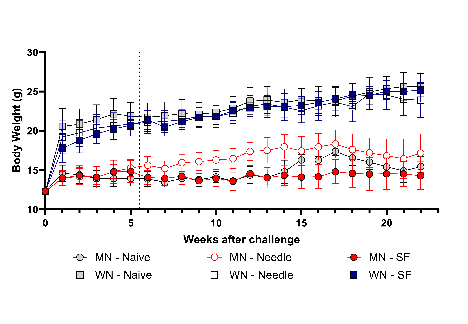
\includegraphics[width=0.9\linewidth,]{Statistics_report_files/figure-latex/call-for-figure-3a-extended-1} 

}

\caption{Fig.3a: This an extended version of the main figure 3a from the publication showing as well the pre-infection time-points. The dotted line marked the point of mouse infection.}\label{fig:call-for-figure-3a-extended}
\end{figure}

We would need to analyze the data with a three-way approach to account for the three predictors, ``Time\_point'' was the within-subject factor, while ``Diet'' and ``Route'' were the between-subject factors in the analysis with ``Weight\_g'' being the dependent outcome variable.

For a three-way mixed ANOVA, we had to assess the data for compliance with assumptions:

\begin{itemize}
\tightlist
\item
  Data normality
\item
  Homogeneity of variance
\item
  No significant outliers
\end{itemize}

Initial assumption assessment indicated that the Gaussian distribution assumption was not met along with the occurrence of several extreme outliers. Data transformation by Box-Cox power transformation reduced the magnitude of violation, although it did not completely remove it. Either way, we present the analysis of the assumption assessment with the transformed data below. Thus, data distribution and variance appear different in the main figure in the publication from the once that were used in the analysis post transformation.

\subsubsection{Assumption analyses}\label{assumption-analyses-2}

\paragraph{Data normality}\label{data-normality-2}

The assessment of the untransformed data distribution for each group was conducted by Shpiro-Wilks test and QQ-plot after splitting the data by all three predictors. Note that all groups consisted of \emph{N}=WN\_Control: 8, MN\_Control: 8, WN\_Needle: 7, MN\_Needle: 7, WN\_SF: 8, MN\_SF: 7 individuals, which made groups too small to assess data distribution reliably by Shapiro-Wilks test. In spite of this, we performed the analyses by Shapiro-Wilks test (Table 87) and QQ-pots (Fig.3a-1) and found deviations from normality.

\begin{longtable}{ccclrrl}
\caption*{
{\large \textbf{Appendix Table 87}} \\ 
{\small \textbf{Univariate Shapito-Wilks test results}}
} \\ 
\toprule
Diet & Route & Time\_point & variable & statistic & p & Outcome \\ 
\midrule\addlinespace[2.5pt]
\multicolumn{7}{l}{Pre-Infection} \\ 
\midrule\addlinespace[2.5pt]
WN & Control & Week\_0 & Counts & 0.7729 & 0.0146 & sig. \\ 
MN & Control & Week\_0 & Counts & 0.9118 & 0.3671 & ns \\ 
WN & Needle & Week\_0 & Counts & 0.6644 & 0.0015 & sig. \\ 
MN & Needle & Week\_0 & Counts & 0.8181 & 0.0615 & ns \\ 
WN & SF & Week\_0 & Counts & 0.7823 & 0.0184 & sig. \\ 
MN & SF & Week\_0 & Counts & 0.8333 & 0.0860 & ns \\ 
WN & Control & Week\_1 & Counts & 0.8468 & 0.0884 & ns \\ 
MN & Control & Week\_1 & Counts & 0.9006 & 0.2923 & ns \\ 
WN & Needle & Week\_1 & Counts & 0.9335 & 0.5814 & ns \\ 
MN & Needle & Week\_1 & Counts & 0.9593 & 0.8128 & ns \\ 
WN & SF & Week\_1 & Counts & 0.8352 & 0.0673 & ns \\ 
MN & SF & Week\_1 & Counts & 0.8678 & 0.1774 & ns \\ 
WN & Control & Week\_2 & Counts & 0.8406 & 0.0764 & ns \\ 
MN & Control & Week\_2 & Counts & 0.8894 & 0.2309 & ns \\ 
WN & Needle & Week\_2 & Counts & 0.9363 & 0.6056 & ns \\ 
MN & Needle & Week\_2 & Counts & 0.8935 & 0.2932 & ns \\ 
WN & SF & Week\_2 & Counts & 0.8253 & 0.0531 & ns \\ 
MN & SF & Week\_2 & Counts & 0.9515 & 0.7437 & ns \\ 
WN & Control & Week\_3 & Counts & 0.8942 & 0.2558 & ns \\ 
MN & Control & Week\_3 & Counts & 0.9273 & 0.4919 & ns \\ 
WN & Needle & Week\_3 & Counts & 0.8753 & 0.2065 & ns \\ 
MN & Needle & Week\_3 & Counts & 0.8073 & 0.0483 & sig. \\ 
WN & SF & Week\_3 & Counts & 0.8960 & 0.2656 & ns \\ 
MN & SF & Week\_3 & Counts & 0.9739 & 0.9249 & ns \\ 
WN & Control & Week\_4 & Counts & 0.9525 & 0.7363 & ns \\ 
MN & Control & Week\_4 & Counts & 0.9198 & 0.4281 & ns \\ 
WN & Needle & Week\_4 & Counts & 0.9146 & 0.4285 & ns \\ 
MN & Needle & Week\_4 & Counts & 0.8741 & 0.2016 & ns \\ 
WN & SF & Week\_4 & Counts & 0.9291 & 0.5079 & ns \\ 
MN & SF & Week\_4 & Counts & 0.9746 & 0.9292 & ns \\ 
WN & Control & Week\_5 & Counts & 0.9659 & 0.8639 & ns \\ 
MN & Control & Week\_5 & Counts & 0.8773 & 0.1773 & ns \\ 
WN & Needle & Week\_5 & Counts & 0.9319 & 0.5674 & ns \\ 
MN & Needle & Week\_5 & Counts & 0.8583 & 0.1463 & ns \\ 
WN & SF & Week\_5 & Counts & 0.9314 & 0.5289 & ns \\ 
MN & SF & Week\_5 & Counts & 0.9633 & 0.8463 & ns \\ 
\midrule\addlinespace[2.5pt]
\multicolumn{7}{l}{Post-Infestion} \\ 
\midrule\addlinespace[2.5pt]
WN & Control & Week\_6 & Counts & 0.9440 & 0.6508 & ns \\ 
MN & Control & Week\_6 & Counts & 0.9299 & 0.5147 & ns \\ 
WN & Needle & Week\_6 & Counts & 0.9699 & 0.8976 & ns \\ 
MN & Needle & Week\_6 & Counts & 0.8327 & 0.0848 & ns \\ 
WN & SF & Week\_6 & Counts & 0.9879 & 0.9911 & ns \\ 
MN & SF & Week\_6 & Counts & 0.9779 & 0.9487 & ns \\ 
WN & Control & Week\_7 & Counts & 0.9637 & 0.8444 & ns \\ 
MN & Control & Week\_7 & Counts & 0.9139 & 0.3825 & ns \\ 
WN & Needle & Week\_7 & Counts & 0.9147 & 0.4296 & ns \\ 
MN & Needle & Week\_7 & Counts & 0.9199 & 0.4688 & ns \\ 
WN & SF & Week\_7 & Counts & 0.9801 & 0.9632 & ns \\ 
MN & SF & Week\_7 & Counts & 0.9295 & 0.5467 & ns \\ 
WN & Control & Week\_8 & Counts & 0.9699 & 0.8969 & ns \\ 
MN & Control & Week\_8 & Counts & 0.9504 & 0.7148 & ns \\ 
WN & Needle & Week\_8 & Counts & 0.9015 & 0.3402 & ns \\ 
MN & Needle & Week\_8 & Counts & 0.8640 & 0.1643 & ns \\ 
WN & SF & Week\_8 & Counts & 0.9431 & 0.6420 & ns \\ 
MN & SF & Week\_8 & Counts & 0.8841 & 0.2453 & ns \\ 
WN & Control & Week\_9 & Counts & 0.9563 & 0.7743 & ns \\ 
MN & Control & Week\_9 & Counts & 0.9378 & 0.5895 & ns \\ 
WN & Needle & Week\_9 & Counts & 0.8770 & 0.2135 & ns \\ 
MN & Needle & Week\_9 & Counts & 0.9078 & 0.3810 & ns \\ 
WN & SF & Week\_9 & Counts & 0.9499 & 0.7105 & ns \\ 
MN & SF & Week\_9 & Counts & 0.9522 & 0.7493 & ns \\ 
WN & Control & Week\_10 & Counts & 0.9366 & 0.5777 & ns \\ 
MN & Control & Week\_10 & Counts & 0.9605 & 0.8145 & ns \\ 
WN & Needle & Week\_10 & Counts & 0.9026 & 0.3472 & ns \\ 
MN & Needle & Week\_10 & Counts & 0.9179 & 0.4533 & ns \\ 
WN & SF & Week\_10 & Counts & 0.9133 & 0.3782 & ns \\ 
MN & SF & Week\_10 & Counts & 0.9534 & 0.7606 & ns \\ 
WN & Control & Week\_11 & Counts & 0.9437 & 0.6478 & ns \\ 
MN & Control & Week\_11 & Counts & 0.9641 & 0.8477 & ns \\ 
WN & Needle & Week\_11 & Counts & 0.9074 & 0.3782 & ns \\ 
MN & Needle & Week\_11 & Counts & 0.8722 & 0.1940 & ns \\ 
WN & SF & Week\_11 & Counts & 0.9294 & 0.5107 & ns \\ 
MN & SF & Week\_11 & Counts & 0.9553 & 0.7771 & ns \\ 
WN & Control & Week\_12 & Counts & 0.9587 & 0.7981 & ns \\ 
MN & Control & Week\_12 & Counts & 0.9428 & 0.6389 & ns \\ 
WN & Needle & Week\_12 & Counts & 0.9434 & 0.6696 & ns \\ 
MN & Needle & Week\_12 & Counts & 0.9293 & 0.5452 & ns \\ 
WN & SF & Week\_12 & Counts & 0.9507 & 0.7186 & ns \\ 
MN & SF & Week\_12 & Counts & 0.9283 & 0.5365 & ns \\ 
WN & Control & Week\_13 & Counts & 0.9768 & 0.9453 & ns \\ 
MN & Control & Week\_13 & Counts & 0.9050 & 0.3205 & ns \\ 
WN & Needle & Week\_13 & Counts & 0.9768 & 0.9426 & ns \\ 
MN & Needle & Week\_13 & Counts & 0.9225 & 0.4887 & ns \\ 
WN & SF & Week\_13 & Counts & 0.9049 & 0.3195 & ns \\ 
MN & SF & Week\_13 & Counts & 0.9002 & 0.3323 & ns \\ 
WN & Control & Week\_14 & Counts & 0.9521 & 0.7323 & ns \\ 
MN & Control & Week\_14 & Counts & 0.8924 & 0.2464 & ns \\ 
WN & Needle & Week\_14 & Counts & 0.9310 & 0.5592 & ns \\ 
MN & Needle & Week\_14 & Counts & 0.9140 & 0.4244 & ns \\ 
WN & SF & Week\_14 & Counts & 0.8788 & 0.1834 & ns \\ 
MN & SF & Week\_14 & Counts & 0.9498 & 0.7279 & ns \\ 
WN & Control & Week\_15 & Counts & 0.9124 & 0.3715 & ns \\ 
MN & Control & Week\_15 & Counts & 0.8167 & 0.0431 & sig. \\ 
WN & Needle & Week\_15 & Counts & 0.7351 & 0.0088 & sig. \\ 
MN & Needle & Week\_15 & Counts & 0.9505 & 0.7338 & ns \\ 
WN & SF & Week\_15 & Counts & 0.9126 & 0.3729 & ns \\ 
MN & SF & Week\_15 & Counts & 0.9603 & 0.8210 & ns \\ 
WN & Control & Week\_16 & Counts & 0.8604 & 0.1212 & ns \\ 
MN & Control & Week\_16 & Counts & 0.8289 & 0.0578 & ns \\ 
WN & Needle & Week\_16 & Counts & 0.7123 & 0.0050 & sig. \\ 
MN & Needle & Week\_16 & Counts & 0.9455 & 0.6885 & ns \\ 
WN & SF & Week\_16 & Counts & 0.8795 & 0.1861 & ns \\ 
MN & SF & Week\_16 & Counts & 0.9444 & 0.6783 & ns \\ 
WN & Control & Week\_17 & Counts & 0.8210 & 0.0478 & sig. \\ 
MN & Control & Week\_17 & Counts & 0.8694 & 0.1487 & ns \\ 
WN & Needle & Week\_17 & Counts & 0.8980 & 0.3190 & ns \\ 
MN & Needle & Week\_17 & Counts & 0.9786 & 0.9522 & ns \\ 
WN & SF & Week\_17 & Counts & 0.8581 & 0.1149 & ns \\ 
MN & SF & Week\_17 & Counts & 0.9189 & 0.4612 & ns \\ 
WN & Control & Week\_18 & Counts & 0.8087 & 0.0354 & sig. \\ 
MN & Control & Week\_18 & Counts & 0.9667 & 0.8713 & ns \\ 
WN & Needle & Week\_18 & Counts & 0.8892 & 0.2706 & ns \\ 
MN & Needle & Week\_18 & Counts & 0.9528 & 0.7550 & ns \\ 
WN & SF & Week\_18 & Counts & 0.8360 & 0.0686 & ns \\ 
MN & SF & Week\_18 & Counts & 0.9453 & 0.6869 & ns \\ 
WN & Control & Week\_19 & Counts & 0.8965 & 0.2689 & ns \\ 
MN & Control & Week\_19 & Counts & 0.9282 & 0.4996 & ns \\ 
WN & Needle & Week\_19 & Counts & 0.6529 & 0.0011 & sig. \\ 
MN & Needle & Week\_19 & Counts & 0.9179 & 0.4532 & ns \\ 
WN & SF & Week\_19 & Counts & 0.8780 & 0.1801 & ns \\ 
MN & SF & Week\_19 & Counts & 0.9285 & 0.5383 & ns \\ 
WN & Control & Week\_20 & Counts & 0.8508 & 0.0971 & ns \\ 
MN & Control & Week\_20 & Counts & 0.9540 & 0.7517 & ns \\ 
WN & Needle & Week\_20 & Counts & 0.7695 & 0.0202 & sig. \\ 
MN & Needle & Week\_20 & Counts & 0.9215 & 0.4808 & ns \\ 
WN & SF & Week\_20 & Counts & 0.8922 & 0.2453 & ns \\ 
MN & SF & Week\_20 & Counts & 0.9223 & 0.4875 & ns \\ 
WN & Control & Week\_21 & Counts & 0.9517 & 0.7285 & ns \\ 
MN & Control & Week\_21 & Counts & 0.9221 & 0.4467 & ns \\ 
WN & Needle & Week\_21 & Counts & 0.8350 & 0.0893 & ns \\ 
MN & Needle & Week\_21 & Counts & 0.9039 & 0.3553 & ns \\ 
WN & SF & Week\_21 & Counts & 0.8391 & 0.0737 & ns \\ 
MN & SF & Week\_21 & Counts & 0.9255 & 0.5133 & ns \\ 
WN & Control & Week\_22 & Counts & 0.9688 & 0.8884 & ns \\ 
MN & Control & Week\_22 & Counts & 0.9392 & 0.6311 & ns \\ 
WN & Needle & Week\_22 & Counts & 0.8309 & 0.0816 & ns \\ 
MN & Needle & Week\_22 & Counts & 0.9453 & 0.6865 & ns \\ 
WN & SF & Week\_22 & Counts & 0.8552 & 0.1075 & ns \\ 
MN & SF & Week\_22 & Counts & 0.9137 & 0.4219 & ns \\ 
\bottomrule
\end{longtable}

\begin{figure}[H]

{\centering 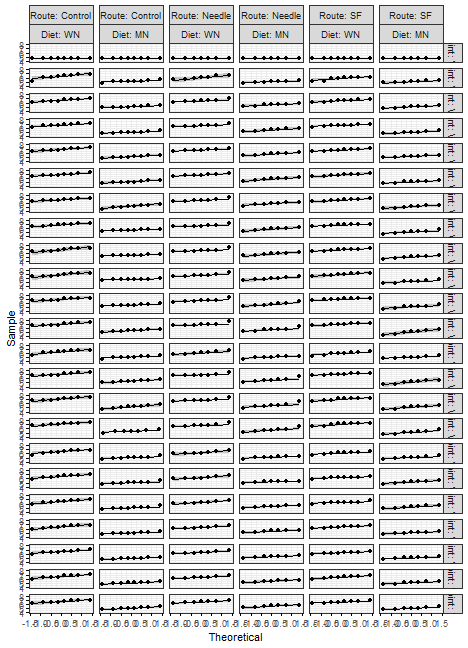
\includegraphics[width=0.95\linewidth,]{Statistics_report_files/figure-latex/qq-plot-figure-3a-1} 

}

\caption{Fig.3a-1: QQ-plots of myeloid cell counts split into groups by predictor variables}\label{fig:qq-plot-figure-3a}
\end{figure}

\paragraph{Homogeneity of variance}\label{homogeneity-of-variance-2}

The assessment of homogeneity of variance was conducted by Levene's test for the dataset split by the within-subject factor (``Time\_point''). The analysis output showed that assumption of homogeneity between groups held for each week (Table 88).

\begin{longtable}{l|rrrrc}
\caption*{
{\large \textbf{Appendix Table 88}} \\ 
{\small \textbf{Assessment of homogeneity of variance by week}}
} \\ 
\toprule
\multicolumn{1}{l}{Weeks p.i.} & df1 & df2 & statistic & p & sig. \\ 
\midrule\addlinespace[2.5pt]
\multicolumn{6}{l}{Pre-Infection} \\ 
\midrule\addlinespace[2.5pt]
Week\_0 & 5 & 39 & 0.5518 & 0.7360 & ns \\ 
Week\_1 & 5 & 39 & 1.2268 & 0.3151 & ns \\ 
Week\_2 & 5 & 39 & 0.4165 & 0.8344 & ns \\ 
Week\_3 & 5 & 39 & 0.3987 & 0.8467 & ns \\ 
Week\_4 & 5 & 39 & 0.8811 & 0.5029 & ns \\ 
Week\_5 & 5 & 39 & 0.6984 & 0.6279 & ns \\ 
\midrule\addlinespace[2.5pt]
\multicolumn{6}{l}{Post-Infestion} \\ 
\midrule\addlinespace[2.5pt]
Week\_6 & 5 & 39 & 1.0550 & 0.3998 & ns \\ 
Week\_7 & 5 & 39 & 1.1844 & 0.3344 & ns \\ 
Week\_8 & 5 & 39 & 0.8324 & 0.5347 & ns \\ 
Week\_9 & 5 & 39 & 0.4061 & 0.8416 & ns \\ 
Week\_10 & 5 & 39 & 0.5260 & 0.7551 & ns \\ 
Week\_11 & 5 & 39 & 0.3293 & 0.8922 & ns \\ 
Week\_12 & 5 & 39 & 0.5888 & 0.7084 & ns \\ 
Week\_13 & 5 & 39 & 0.2664 & 0.9287 & ns \\ 
Week\_14 & 5 & 39 & 0.1285 & 0.9850 & ns \\ 
Week\_15 & 5 & 39 & 0.8254 & 0.5393 & ns \\ 
Week\_16 & 5 & 39 & 1.5470 & 0.1979 & ns \\ 
Week\_17 & 5 & 39 & 1.6538 & 0.1688 & ns \\ 
Week\_18 & 5 & 39 & 0.9135 & 0.4824 & ns \\ 
Week\_19 & 5 & 39 & 0.7931 & 0.5612 & ns \\ 
Week\_20 & 5 & 39 & 0.9508 & 0.4595 & ns \\ 
Week\_21 & 5 & 39 & 0.2343 & 0.9451 & ns \\ 
Week\_22 & 5 & 38 & 0.3294 & 0.8921 & ns \\ 
\bottomrule
\end{longtable}

\paragraph{Outliers}\label{outliers-2}

It can be difficult to determine outliers in small datasets reliably as the analysis is dependent on the interquartile range of the data per group. We attempted it anyway and found a total of 53 hypothetical outliers of which 7 were classed as extreme (Table 89).

\begin{longtable}{ccccc}
\caption*{
{\large \textbf{Appendix Table 89}} \\ 
{\small \textbf{List of possible outliers}}
} \\ 
\toprule
Diet & Route & Time\_point & is.outlier & is.extreme \\ 
\midrule\addlinespace[2.5pt]
\multicolumn{5}{l}{Pre-Infection} \\ 
\midrule\addlinespace[2.5pt]
WN & Control & Week\_0 & TRUE & FALSE \\ 
WN & Control & Week\_1 & TRUE & FALSE \\ 
MN & Control & Week\_1 & TRUE & FALSE \\ 
MN & Control & Week\_1 & TRUE & TRUE \\ 
MN & Needle & Week\_1 & TRUE & FALSE \\ 
WN & SF & Week\_1 & TRUE & FALSE \\ 
MN & Control & Week\_2 & TRUE & FALSE \\ 
MN & Control & Week\_2 & TRUE & TRUE \\ 
WN & SF & Week\_2 & TRUE & FALSE \\ 
WN & SF & Week\_2 & TRUE & FALSE \\ 
MN & SF & Week\_2 & TRUE & FALSE \\ 
WN & Control & Week\_3 & TRUE & FALSE \\ 
MN & Control & Week\_3 & TRUE & FALSE \\ 
MN & Control & Week\_3 & TRUE & FALSE \\ 
MN & Needle & Week\_3 & TRUE & FALSE \\ 
WN & SF & Week\_3 & TRUE & FALSE \\ 
MN & SF & Week\_3 & TRUE & FALSE \\ 
MN & Control & Week\_4 & TRUE & FALSE \\ 
MN & Control & Week\_4 & TRUE & FALSE \\ 
MN & Needle & Week\_4 & TRUE & TRUE \\ 
WN & SF & Week\_4 & TRUE & FALSE \\ 
MN & Control & Week\_5 & TRUE & TRUE \\ 
MN & Control & Week\_5 & TRUE & FALSE \\ 
WN & SF & Week\_5 & TRUE & FALSE \\ 
WN & SF & Week\_5 & TRUE & FALSE \\ 
\midrule\addlinespace[2.5pt]
\multicolumn{5}{l}{Post-Infestion} \\ 
\midrule\addlinespace[2.5pt]
MN & Control & Week\_6 & TRUE & FALSE \\ 
MN & Control & Week\_6 & TRUE & FALSE \\ 
WN & SF & Week\_9 & TRUE & FALSE \\ 
WN & Needle & Week\_10 & TRUE & FALSE \\ 
WN & Needle & Week\_11 & TRUE & FALSE \\ 
WN & SF & Week\_11 & TRUE & FALSE \\ 
WN & Needle & Week\_12 & TRUE & FALSE \\ 
WN & Needle & Week\_14 & TRUE & FALSE \\ 
MN & Control & Week\_15 & TRUE & FALSE \\ 
WN & Needle & Week\_15 & TRUE & FALSE \\ 
WN & SF & Week\_15 & TRUE & FALSE \\ 
MN & SF & Week\_15 & TRUE & FALSE \\ 
MN & Control & Week\_16 & TRUE & FALSE \\ 
WN & Needle & Week\_16 & TRUE & TRUE \\ 
MN & Control & Week\_17 & TRUE & FALSE \\ 
WN & Needle & Week\_17 & TRUE & FALSE \\ 
MN & Control & Week\_18 & TRUE & FALSE \\ 
WN & Needle & Week\_18 & TRUE & FALSE \\ 
WN & Needle & Week\_19 & TRUE & TRUE \\ 
MN & Needle & Week\_19 & TRUE & FALSE \\ 
WN & Needle & Week\_20 & TRUE & TRUE \\ 
MN & Needle & Week\_20 & TRUE & FALSE \\ 
WN & Needle & Week\_21 & TRUE & FALSE \\ 
MN & Needle & Week\_21 & TRUE & FALSE \\ 
MN & Control & Week\_22 & TRUE & FALSE \\ 
MN & Control & Week\_22 & TRUE & FALSE \\ 
WN & Needle & Week\_22 & TRUE & FALSE \\ 
MN & Needle & Week\_22 & TRUE & FALSE \\ 
\bottomrule
\end{longtable}

\subsubsection{Three-way analysis}\label{three-way-analysis-2}

Based on the assumption analysis, we decided to apply a Robust three-way ANOVA to the dataset to determine the effects of ``Diet'', infection ``Route'' and time post infection (``Time\_point'') on mouse weight over time (Table 90). The test output showed that all three individual predictors were a statistically significant, while only the two two-way interactions with ``Diet'' were statistically significant. There was no statistically significant three-way interaction.

\begin{longtable}{l|rrc}
\caption*{
{\large \textbf{Appendix Table 90}} \\ 
{\small \textbf{Robust three-way mixed ANOVA}}
} \\ 
\toprule
\multicolumn{1}{l}{Predictors} & value & p.value & sig. \\ 
\midrule\addlinespace[2.5pt]
Diet & 4726.0759 & 0.0001 & **** \\ 
Route & 53.7814 & 0.0001 & **** \\ 
Time\_point & 15104.9064 & 0.0010 & *** \\ 
Diet:Route & 155.4204 & 0.0010 & *** \\ 
Diet:Time\_point & 4280.0234 & 0.0010 & *** \\ 
Route:Time\_point & 106.9048 & 0.0010 & *** \\ 
Diet:Route:Time\_point & 204.8501 & 0.0010 & *** \\ 
\bottomrule
\end{longtable}

We looked for main effects by splitting the data by te within-subject factor (``Time\_point'') and analyzed the remaining two predictor (``Diet'' and ``Roue'') by a Robust two-way ANOVA. The results showed that both predictors, ``Diet'' and ``Route'', produced statistically significant p-values. While ``Diet'' had always statistical significance with the exception of ``Week\_0'', which was unsurprising considering the large gap in body weight between well-nourished and malnourished mice otherwise throughout the observation period (Fig. 3a). ``Route'' was only a statistically significant predictor between ``Week\_9'' and ``Week\_17'', and the interaction term was statistically significant between ``Week\_7'' and ``Week\_18'' (Table 91). This suggested that the effects of the Route'' of infection were only observed for a limited period of time post infection, while the effects of ``Diet'' were predefined at the point of infection. The interaction suggests that within one or both dietary groups statistically significant differences were observed due to infection route.

\begin{longtable}{l|lrrc}
\caption*{
{\large \textbf{Appendix Table 91}} \\ 
{\small \textbf{Robust two-way ANOVA}}
} \\ 
\toprule
\multicolumn{1}{l}{Weeks p.i.} & Predictor & value & p.value & Sig. \\ 
\midrule\addlinespace[2.5pt]
\multicolumn{5}{l}{Pre-Infection} \\ 
\midrule\addlinespace[2.5pt]
Week\_0 & Diet & 0.6436 & 0.429 & ns \\ 
Week\_0 & Route & 4.8913 & 0.116 & ns \\ 
Week\_0 & Diet:Route & 0.5024 & 0.786 & ns \\ 
Week\_1 & Diet & 83.2007 & 0.001 & *** \\ 
Week\_1 & Route & 5.6282 & 0.088 & + \\ 
Week\_1 & Diet:Route & 2.2941 & 0.349 & ns \\ 
Week\_2 & Diet & 128.0593 & 0.001 & *** \\ 
Week\_2 & Route & 2.6197 & 0.298 & ns \\ 
Week\_2 & Diet:Route & 2.3070 & 0.342 & ns \\ 
Week\_3 & Diet & 187.7605 & 0.001 & *** \\ 
Week\_3 & Route & 1.5396 & 0.484 & ns \\ 
Week\_3 & Diet:Route & 2.3585 & 0.335 & ns \\ 
Week\_4 & Diet & 192.4720 & 0.001 & *** \\ 
Week\_4 & Route & 0.3976 & 0.826 & ns \\ 
Week\_4 & Diet:Route & 6.0356 & 0.073 & + \\ 
Week\_5 & Diet & 212.5551 & 0.001 & *** \\ 
Week\_5 & Route & 0.4535 & 0.804 & ns \\ 
Week\_5 & Diet:Route & 5.4285 & 0.091 & + \\ 
\midrule\addlinespace[2.5pt]
\multicolumn{5}{l}{Post-Infestion} \\ 
\midrule\addlinespace[2.5pt]
Week\_6 & Diet & 262.5681 & 0.001 & *** \\ 
Week\_6 & Route & 2.5042 & 0.313 & ns \\ 
Week\_6 & Diet:Route & 6.2856 & 0.064 & + \\ 
Week\_7 & Diet & 330.1662 & 0.001 & *** \\ 
Week\_7 & Route & 5.1005 & 0.106 & ns \\ 
Week\_7 & Diet:Route & 7.2688 & 0.045 & * \\ 
Week\_8 & Diet & 263.7557 & 0.001 & *** \\ 
Week\_8 & Route & 4.9514 & 0.110 & ns \\ 
Week\_8 & Diet:Route & 7.9498 & 0.034 & * \\ 
Week\_9 & Diet & 335.2713 & 0.001 & *** \\ 
Week\_9 & Route & 8.9642 & 0.023 & * \\ 
Week\_9 & Diet:Route & 9.4158 & 0.019 & * \\ 
Week\_10 & Diet & 304.2046 & 0.001 & *** \\ 
Week\_10 & Route & 6.7550 & 0.053 & + \\ 
Week\_10 & Diet:Route & 9.4577 & 0.019 & * \\ 
Week\_11 & Diet & 378.3575 & 0.001 & *** \\ 
Week\_11 & Route & 10.0779 & 0.016 & * \\ 
Week\_11 & Diet:Route & 16.3481 & 0.002 & ** \\ 
Week\_12 & Diet & 326.4604 & 0.001 & *** \\ 
Week\_12 & Route & 12.5730 & 0.006 & ** \\ 
Week\_12 & Diet:Route & 14.7796 & 0.003 & ** \\ 
Week\_13 & Diet & 302.1738 & 0.001 & *** \\ 
Week\_13 & Route & 13.4748 & 0.005 & ** \\ 
Week\_13 & Diet:Route & 14.6520 & 0.004 & ** \\ 
Week\_14 & Diet & 208.9694 & 0.001 & *** \\ 
Week\_14 & Route & 10.6331 & 0.013 & * \\ 
Week\_14 & Diet:Route & 13.2573 & 0.005 & ** \\ 
Week\_15 & Diet & 231.8533 & 0.001 & *** \\ 
Week\_15 & Route & 10.0367 & 0.017 & * \\ 
Week\_15 & Diet:Route & 11.3226 & 0.011 & * \\ 
Week\_16 & Diet & 210.5225 & 0.001 & *** \\ 
Week\_16 & Route & 8.7925 & 0.026 & * \\ 
Week\_16 & Diet:Route & 11.9954 & 0.009 & ** \\ 
Week\_17 & Diet & 177.0197 & 0.001 & *** \\ 
Week\_17 & Route & 7.6225 & 0.040 & * \\ 
Week\_17 & Diet:Route & 11.2424 & 0.011 & * \\ 
Week\_18 & Diet & 208.5641 & 0.001 & *** \\ 
Week\_18 & Route & 3.5529 & 0.204 & ns \\ 
Week\_18 & Diet:Route & 11.4103 & 0.011 & * \\ 
Week\_19 & Diet & 230.7852 & 0.001 & *** \\ 
Week\_19 & Route & 4.5003 & 0.139 & ns \\ 
Week\_19 & Diet:Route & 3.4689 & 0.212 & ns \\ 
Week\_20 & Diet & 259.4895 & 0.001 & *** \\ 
Week\_20 & Route & 2.0155 & 0.395 & ns \\ 
Week\_20 & Diet:Route & 4.1171 & 0.163 & ns \\ 
Week\_21 & Diet & 227.8845 & 0.001 & *** \\ 
Week\_21 & Route & 0.7795 & 0.689 & ns \\ 
Week\_21 & Diet:Route & 4.3443 & 0.143 & ns \\ 
Week\_22 & Diet & 215.7785 & 0.001 & *** \\ 
Week\_22 & Route & 2.1574 & 0.367 & ns \\ 
Week\_22 & Diet:Route & 7.1401 & 0.048 & * \\ 
\bottomrule
\end{longtable}

For the analysis of the simple simple main effect for each respective between-subject factor, we performed Robust one-way ANOVA with individual between-subject factor of the data split by the other two predictors. The results showed that ``Diet'' caused statistically significant differences with the exception of ``Week\_0'', which prior to the assignment of special diets (Table 92). ``Route only showed occasionally statistical significant difference; most commonly between''Week\_6'' and ``Week\_18'', which was only associated with the malnourished group (Table 93).

\begin{longtable}{lllrrrlrrrc}
\caption*{
{\large \textbf{Appendix Table 92}} \\ 
{\small \textbf{Robust one-way ANOVA}}
} \\ 
\toprule
Time\_point & Factor & Effect & test & df1 & df2 & p.value & effsize & CI\_lower & CI\_upper & Sig. \\ 
\midrule\addlinespace[2.5pt]
\multicolumn{11}{l}{Split by Route} \\ 
\midrule\addlinespace[2.5pt]
Week\_0 & Control & Diet & 0.9463 & 1 & 13.9443 & 0.3472 & 0.3265 & 0.0009 & 0.7239 & ns \\ 
Week\_0 & Needle & Diet & 0.0742 & 1 & 8.1104 & 0.7921 & 0.0880 & 0.0018 & 0.8640 & ns \\ 
Week\_0 & SF & Diet & 0.0073 & 1 & 12.9968 & 0.9334 & 0.2208 & 0.0000 & 0.6874 & ns \\ 
Week\_1 & Control & Diet & 30.9197 & 1 & 10.5864 & 0.0002 & 0.9867 & 0.7579 & 1.1607 & *** \\ 
Week\_1 & Needle & Diet & 33.6082 & 1 & 8.7119 & 0.0003 & 1.0360 & 0.9235 & 1.1585 & *** \\ 
Week\_1 & SF & Diet & 19.4931 & 1 & 10.7930 & 0.0011 & 0.9022 & 0.5425 & 1.0997 & ** \\ 
Week\_2 & Control & Diet & 46.6180 & 1 & 12.5452 & <0.0001 & 1.0575 & 0.9074 & 1.1649 & **** \\ 
Week\_2 & Needle & Diet & 49.7907 & 1 & 10.7859 & <0.0001 & 1.0994 & 0.9863 & 1.2523 & **** \\ 
Week\_2 & SF & Diet & 32.7851 & 1 & 11.8409 & 0.0001 & 0.9999 & 0.8331 & 1.1639 & *** \\ 
Week\_3 & Control & Diet & 71.4565 & 1 & 12.4770 & <0.0001 & 1.0818 & 0.9760 & 1.1524 & **** \\ 
Week\_3 & Needle & Diet & 66.2027 & 1 & 10.2527 & <0.0001 & 1.1338 & 1.0156 & 1.2552 & **** \\ 
Week\_3 & SF & Diet & 50.8531 & 1 & 11.8824 & <0.0001 & 1.0649 & 0.9792 & 1.1777 & **** \\ 
Week\_4 & Control & Diet & 87.8417 & 1 & 12.1493 & <0.0001 & 1.1032 & 1.0040 & 1.1413 & **** \\ 
Week\_4 & Needle & Diet & 60.9978 & 1 & 10.2379 & <0.0001 & 1.1344 & 1.0132 & 1.2331 & **** \\ 
Week\_4 & SF & Diet & 45.9854 & 1 & 11.0139 & <0.0001 & 1.0600 & 0.9189 & 1.1884 & **** \\ 
Week\_5 & Control & Diet & 100.3686 & 1 & 12.7279 & <0.0001 & 1.1053 & 1.0363 & 1.1542 & **** \\ 
Week\_5 & Needle & Diet & 56.4055 & 1 & 11.6501 & <0.0001 & 1.0898 & 0.9942 & 1.2567 & **** \\ 
Week\_5 & SF & Diet & 58.6004 & 1 & 10.7527 & <0.0001 & 1.0839 & 0.9806 & 1.2003 & **** \\ 
Week\_6 & Control & Diet & 88.8819 & 1 & 12.0825 & <0.0001 & 1.0922 & 1.0234 & 1.1534 & **** \\ 
Week\_6 & Needle & Diet & 54.4571 & 1 & 11.9346 & <0.0001 & 1.0689 & 0.9799 & 1.2291 & **** \\ 
Week\_6 & SF & Diet & 138.7395 & 1 & 12.9947 & <0.0001 & 1.1099 & 1.0636 & 1.1608 & **** \\ 
Week\_7 & Control & Diet & 139.0888 & 1 & 9.6090 & <0.0001 & 1.1113 & 1.0622 & 1.1520 & **** \\ 
Week\_7 & Needle & Diet & 79.5424 & 1 & 11.6833 & <0.0001 & 1.1279 & 1.0372 & 1.2009 & **** \\ 
Week\_7 & SF & Diet & 115.0358 & 1 & 12.9933 & <0.0001 & 1.1055 & 1.0434 & 1.1664 & **** \\ 
Week\_8 & Control & Diet & 108.6133 & 1 & 11.1301 & <0.0001 & 1.1069 & 1.0373 & 1.1390 & **** \\ 
Week\_8 & Needle & Diet & 64.9819 & 1 & 11.9851 & <0.0001 & 1.1008 & 1.0198 & 1.1840 & **** \\ 
Week\_8 & SF & Diet & 90.4757 & 1 & 12.9631 & <0.0001 & 1.0930 & 1.0282 & 1.1714 & **** \\ 
Week\_9 & Control & Diet & 138.2405 & 1 & 12.6407 & <0.0001 & 1.0938 & 1.0567 & 1.1317 & **** \\ 
Week\_9 & Needle & Diet & 59.2647 & 1 & 11.9764 & <0.0001 & 1.1281 & 1.0054 & 1.2280 & **** \\ 
Week\_9 & SF & Diet & 156.4098 & 1 & 12.9750 & <0.0001 & 1.1141 & 1.0647 & 1.1674 & **** \\ 
Week\_10 & Control & Diet & 142.1475 & 1 & 11.3023 & <0.0001 & 1.1193 & 1.0511 & 1.1490 & **** \\ 
Week\_10 & Needle & Diet & 56.2825 & 1 & 11.9764 & <0.0001 & 1.1457 & 1.0089 & 1.2562 & **** \\ 
Week\_10 & SF & Diet & 118.0082 & 1 & 12.9925 & <0.0001 & 1.0907 & 1.0405 & 1.1480 & **** \\ 
Week\_11 & Control & Diet & 184.1228 & 1 & 12.2479 & <0.0001 & 1.0992 & 1.0666 & 1.1448 & **** \\ 
Week\_11 & Needle & Diet & 59.3268 & 1 & 11.7074 & <0.0001 & 1.1027 & 1.0133 & 1.2393 & **** \\ 
Week\_11 & SF & Diet & 158.6371 & 1 & 12.1492 & <0.0001 & 1.1072 & 1.0679 & 1.1475 & **** \\ 
Week\_12 & Control & Diet & 124.1778 & 1 & 13.5899 & <0.0001 & 1.1083 & 1.0484 & 1.1454 & **** \\ 
Week\_12 & Needle & Diet & 63.5146 & 1 & 11.9642 & <0.0001 & 1.1025 & 1.0221 & 1.2193 & **** \\ 
Week\_12 & SF & Diet & 148.2799 & 1 & 12.9212 & <0.0001 & 1.1048 & 1.0781 & 1.1607 & **** \\ 
Week\_13 & Control & Diet & 159.1247 & 1 & 12.9562 & <0.0001 & 1.1146 & 1.0659 & 1.1539 & **** \\ 
Week\_13 & Needle & Diet & 43.9328 & 1 & 11.0735 & <0.0001 & 1.0647 & 0.9797 & 1.2014 & **** \\ 
Week\_13 & SF & Diet & 124.1739 & 1 & 12.1224 & <0.0001 & 1.0937 & 1.0459 & 1.1608 & **** \\ 
Week\_14 & Control & Diet & 81.6612 & 1 & 13.7559 & <0.0001 & 1.1121 & 1.0289 & 1.1862 & **** \\ 
Week\_14 & Needle & Diet & 28.2635 & 1 & 11.9462 & 0.0002 & 1.1630 & 0.9098 & 1.2623 & *** \\ 
Week\_14 & SF & Diet & 121.5173 & 1 & 12.1033 & <0.0001 & 1.0929 & 1.0455 & 1.1470 & **** \\ 
Week\_15 & Control & Diet & 132.8303 & 1 & 11.5452 & <0.0001 & 1.1446 & 1.0555 & 1.1641 & **** \\ 
Week\_15 & Needle & Diet & 26.5980 & 1 & 10.6701 & 0.0003 & 1.1250 & 0.8928 & 1.3944 & *** \\ 
Week\_15 & SF & Diet & 127.4723 & 1 & 10.3884 & <0.0001 & 1.1094 & 1.0361 & 1.1579 & **** \\ 
Week\_16 & Control & Diet & 100.3834 & 1 & 8.4872 & <0.0001 & 1.0950 & 1.0457 & 1.1333 & **** \\ 
Week\_16 & Needle & Diet & 27.3372 & 1 & 11.9350 & 0.0002 & 1.1261 & 0.9201 & 1.2388 & *** \\ 
Week\_16 & SF & Diet & 110.7167 & 1 & 11.2457 & <0.0001 & 1.0967 & 1.0502 & 1.1709 & **** \\ 
Week\_17 & Control & Diet & 69.5823 & 1 & 8.7894 & <0.0001 & 1.0702 & 1.0164 & 1.1259 & **** \\ 
Week\_17 & Needle & Diet & 25.4983 & 1 & 11.8638 & 0.0003 & 1.0843 & 0.8552 & 1.2132 & *** \\ 
Week\_17 & SF & Diet & 104.7430 & 1 & 11.4557 & <0.0001 & 1.0962 & 1.0511 & 1.1639 & **** \\ 
Week\_18 & Control & Diet & 108.3643 & 1 & 12.9680 & <0.0001 & 1.0997 & 1.0550 & 1.1702 & **** \\ 
Week\_18 & Needle & Diet & 23.9856 & 1 & 11.6560 & 0.0004 & 1.0855 & 0.8390 & 1.2260 & *** \\ 
Week\_18 & SF & Diet & 123.5300 & 1 & 7.7478 & <0.0001 & 1.0956 & 1.0486 & 1.1685 & **** \\ 
Week\_19 & Control & Diet & 133.9525 & 1 & 12.8372 & <0.0001 & 1.0831 & 1.0591 & 1.1506 & **** \\ 
Week\_19 & Needle & Diet & 46.3485 & 1 & 11.7773 & <0.0001 & 1.1568 & 0.9677 & 1.2498 & **** \\ 
Week\_19 & SF & Diet & 82.2076 & 1 & 7.9091 & <0.0001 & 1.0804 & 1.0251 & 1.1832 & **** \\ 
Week\_20 & Control & Diet & 157.5335 & 1 & 13.9259 & <0.0001 & 1.0929 & 1.0730 & 1.1631 & **** \\ 
Week\_20 & Needle & Diet & 44.7878 & 1 & 10.7340 & <0.0001 & 1.1444 & 0.9522 & 1.2082 & **** \\ 
Week\_20 & SF & Diet & 99.9882 & 1 & 7.8372 & <0.0001 & 1.0933 & 1.0481 & 1.1832 & **** \\ 
Week\_21 & Control & Diet & 113.5715 & 1 & 13.8178 & <0.0001 & 1.0896 & 1.0582 & 1.1729 & **** \\ 
Week\_21 & Needle & Diet & 33.1991 & 1 & 10.5972 & 0.0001 & 1.0890 & 0.8607 & 1.2207 & *** \\ 
Week\_21 & SF & Diet & 121.3469 & 1 & 11.0681 & <0.0001 & 1.1009 & 1.0605 & 1.1678 & **** \\ 
Week\_22 & Control & Diet & 136.2265 & 1 & 12.9780 & <0.0001 & 1.1126 & 1.0586 & 1.1811 & **** \\ 
Week\_22 & Needle & Diet & 25.6731 & 1 & 11.1438 & 0.0003 & 1.0823 & 0.7903 & 1.2356 & *** \\ 
Week\_22 & SF & Diet & 111.3334 & 1 & 10.6612 & <0.0001 & 1.0940 & 1.0386 & 1.1744 & **** \\ 
\midrule\addlinespace[2.5pt]
\multicolumn{11}{l}{Split by Diet} \\ 
\midrule\addlinespace[2.5pt]
Week\_0 & WN & Route & 1.9588 & 2 & 12.8725 & 0.1808 & 0.4893 & 0.1490 & 0.8093 & ns \\ 
Week\_0 & MN & Route & 1.0762 & 2 & 12.1312 & 0.3713 & 0.4805 & 0.1011 & 0.8476 & ns \\ 
Week\_1 & WN & Route & 2.2567 & 2 & 13.2118 & 0.1435 & 0.5778 & 0.2353 & 0.9016 & ns \\ 
Week\_1 & MN & Route & 0.6409 & 2 & 12.6553 & 0.5431 & 0.4520 & 0.0778 & 0.9168 & ns \\ 
Week\_2 & WN & Route & 1.6924 & 2 & 13.2826 & 0.2215 & 0.5245 & 0.1950 & 0.8207 & ns \\ 
Week\_2 & MN & Route & 0.0597 & 2 & 12.6611 & 0.9423 & 0.3626 & 0.0496 & 0.9067 & ns \\ 
Week\_3 & WN & Route & 1.6823 & 2 & 12.8046 & 0.2245 & 0.5462 & 0.1318 & 0.8698 & ns \\ 
Week\_3 & MN & Route & 0.0564 & 2 & 12.3027 & 0.9454 & 0.3494 & 0.0647 & 0.9018 & ns \\ 
Week\_4 & WN & Route & 1.8918 & 2 & 12.7117 & 0.1909 & 0.5329 & 0.1169 & 0.8900 & ns \\ 
Week\_4 & MN & Route & 1.3314 & 2 & 12.1316 & 0.3001 & 0.5199 & 0.1351 & 0.9043 & ns \\ 
Week\_5 & WN & Route & 0.8912 & 2 & 12.7927 & 0.4342 & 0.4278 & 0.0860 & 0.8367 & ns \\ 
Week\_5 & MN & Route & 2.4199 & 2 & 12.2564 & 0.1301 & 0.5479 & 0.1046 & 0.8873 & ns \\ 
Week\_6 & WN & Route & 0.2057 & 2 & 12.9847 & 0.8167 & 0.3726 & 0.0547 & 0.7028 & ns \\ 
Week\_6 & MN & Route & 4.6012 & 2 & 12.5486 & 0.0317 & 0.7071 & 0.3539 & 0.9990 & * \\ 
Week\_7 & WN & Route & 1.3374 & 2 & 13.0307 & 0.2963 & 0.4659 & 0.0746 & 0.8409 & ns \\ 
Week\_7 & MN & Route & 6.6197 & 2 & 11.8250 & 0.0118 & 0.7229 & 0.4533 & 0.9427 & * \\ 
Week\_8 & WN & Route & 0.5185 & 2 & 13.2073 & 0.6070 & 0.3676 & 0.0697 & 0.7614 & ns \\ 
Week\_8 & MN & Route & 6.4573 & 2 & 12.2947 & 0.0121 & 0.7206 & 0.5076 & 0.9312 & * \\ 
Week\_9 & WN & Route & 0.0958 & 2 & 13.2133 & 0.9093 & 0.3300 & 0.0387 & 0.7494 & ns \\ 
Week\_9 & MN & Route & 9.4920 & 2 & 12.4183 & 0.0032 & 0.7882 & 0.6314 & 0.9290 & ** \\ 
Week\_10 & WN & Route & 0.2026 & 2 & 13.3101 & 0.8191 & 0.3207 & 0.0838 & 0.7937 & ns \\ 
Week\_10 & MN & Route & 7.8905 & 2 & 11.8254 & 0.0067 & 0.7947 & 0.5708 & 0.9749 & ** \\ 
Week\_11 & WN & Route & 0.2315 & 2 & 13.2266 & 0.7965 & 0.3586 & 0.1059 & 0.7313 & ns \\ 
Week\_11 & MN & Route & 11.6677 & 2 & 11.8647 & 0.0016 & 0.8443 & 0.7023 & 0.9919 & ** \\ 
Week\_12 & WN & Route & 0.3790 & 2 & 13.2137 & 0.6918 & 0.3645 & 0.0436 & 0.7253 & ns \\ 
Week\_12 & MN & Route & 12.5813 & 2 & 12.6487 & 0.0010 & 0.8631 & 0.7246 & 1.0332 & *** \\ 
Week\_13 & WN & Route & 0.3800 & 2 & 13.2733 & 0.6911 & 0.3427 & 0.0785 & 0.7311 & ns \\ 
Week\_13 & MN & Route & 11.0540 & 2 & 11.9483 & 0.0019 & 0.8523 & 0.7450 & 0.9947 & ** \\ 
Week\_14 & WN & Route & 0.1990 & 2 & 13.0343 & 0.8220 & 0.2911 & 0.0397 & 0.7604 & ns \\ 
Week\_14 & MN & Route & 10.1230 & 2 & 12.6525 & 0.0024 & 0.8325 & 0.6854 & 1.0012 & ** \\ 
Week\_15 & WN & Route & 1.2098 & 2 & 12.9990 & 0.3297 & 0.5001 & 0.1221 & 0.8663 & ns \\ 
Week\_15 & MN & Route & 6.6894 & 2 & 10.4184 & 0.0135 & 0.8531 & 0.5907 & 1.0766 & * \\ 
Week\_16 & WN & Route & 0.1823 & 2 & 13.0098 & 0.8354 & 0.3426 & 0.0731 & 0.7330 & ns \\ 
Week\_16 & MN & Route & 7.9104 & 2 & 9.3879 & 0.0097 & 0.9453 & 0.7688 & 1.1793 & ** \\ 
Week\_17 & WN & Route & 0.1053 & 2 & 12.9985 & 0.9008 & 0.2752 & 0.0438 & 0.7046 & ns \\ 
Week\_17 & MN & Route & 7.7361 & 2 & 9.5588 & 0.0100 & 0.9891 & 0.7925 & 1.2656 & * \\ 
Week\_18 & WN & Route & 1.4892 & 2 & 11.5452 & 0.2659 & 0.4710 & 0.1032 & 0.8207 & ns \\ 
Week\_18 & MN & Route & 4.0466 & 2 & 10.9429 & 0.0484 & 0.8530 & 0.4328 & 1.1840 & * \\ 
Week\_19 & WN & Route & 0.1186 & 2 & 12.3347 & 0.8891 & 0.3585 & 0.0571 & 0.7342 & ns \\ 
Week\_19 & MN & Route & 2.5349 & 2 & 10.7215 & 0.1255 & 0.7664 & 0.2584 & 1.2106 & ns \\ 
Week\_20 & WN & Route & 0.3121 & 2 & 12.3417 & 0.7375 & 0.3788 & 0.0410 & 0.8568 & ns \\ 
Week\_20 & MN & Route & 1.7845 & 2 & 11.1498 & 0.2126 & 0.7201 & 0.1120 & 1.2486 & ns \\ 
Week\_21 & WN & Route & 0.9900 & 2 & 12.8920 & 0.3981 & 0.4395 & 0.0749 & 0.7919 & ns \\ 
Week\_21 & MN & Route & 1.2693 & 2 & 12.1936 & 0.3157 & 0.5648 & 0.1110 & 0.9098 & ns \\ 
Week\_22 & WN & Route & 1.1111 & 2 & 12.8371 & 0.3589 & 0.4654 & 0.1060 & 0.8061 & ns \\ 
Week\_22 & MN & Route & 2.6553 & 2 & 11.3155 & 0.1134 & 0.7444 & 0.4043 & 1.2335 & ns \\ 
\bottomrule
\end{longtable}

\begin{longtable}{lllrrrrrrrc}
\caption*{
{\large \textbf{Appendix Table 93}} \\ 
{\small \textbf{Robust one-way ANOVA - sig. summary}}
} \\ 
\toprule
Time\_point & Factor & Effect & test & df1 & df2 & p.value & effsize & CI\_lower & CI\_upper & Sig. \\ 
\midrule\addlinespace[2.5pt]
Week\_6 & MN & Route & 4.6012 & 2 & 12.5486 & 0.0317 & 0.7071 & 0.3539 & 0.9990 & * \\ 
Week\_7 & MN & Route & 6.6197 & 2 & 11.8250 & 0.0118 & 0.7229 & 0.4533 & 0.9427 & * \\ 
Week\_8 & MN & Route & 6.4573 & 2 & 12.2947 & 0.0121 & 0.7206 & 0.5076 & 0.9312 & * \\ 
Week\_9 & MN & Route & 9.4920 & 2 & 12.4183 & 0.0032 & 0.7882 & 0.6314 & 0.9290 & ** \\ 
Week\_10 & MN & Route & 7.8905 & 2 & 11.8254 & 0.0067 & 0.7947 & 0.5708 & 0.9749 & ** \\ 
Week\_11 & MN & Route & 11.6677 & 2 & 11.8647 & 0.0016 & 0.8443 & 0.7023 & 0.9919 & ** \\ 
Week\_12 & MN & Route & 12.5813 & 2 & 12.6487 & 0.0010 & 0.8631 & 0.7246 & 1.0332 & *** \\ 
Week\_13 & MN & Route & 11.0540 & 2 & 11.9483 & 0.0019 & 0.8523 & 0.7450 & 0.9947 & ** \\ 
Week\_14 & MN & Route & 10.1230 & 2 & 12.6525 & 0.0024 & 0.8325 & 0.6854 & 1.0012 & ** \\ 
Week\_15 & MN & Route & 6.6894 & 2 & 10.4184 & 0.0135 & 0.8531 & 0.5907 & 1.0766 & * \\ 
Week\_16 & MN & Route & 7.9104 & 2 & 9.3879 & 0.0097 & 0.9453 & 0.7688 & 1.1793 & ** \\ 
Week\_17 & MN & Route & 7.7361 & 2 & 9.5588 & 0.0100 & 0.9891 & 0.7925 & 1.2656 & * \\ 
Week\_18 & MN & Route & 4.0466 & 2 & 10.9429 & 0.0484 & 0.8530 & 0.4328 & 1.1840 & * \\ 
\bottomrule
\end{longtable}

For the pairwise comparison, we applied a Linear contrast expression. Since the ``Diet'' predictor only had two factor levels, the output showed the same result as the Robust one-way ANOVA above. For the ``Route'' predictor, the pairwise comparison presented a more detailed view at where statistically significant differences occurred (Table 94). As for the Robust one-way ANOVA above, all statistical significant differences were observed between ``Week\_6'' and ``Week\_18'' and were restricted to the malnourished groups (Table 95). The main differences between the malnourished groups resided primarily with the needle inoculated group from ``Week\_6'' to ``Week\_14'', who had more weight gain than either the malnourished control or sand fly infected groups. From ``Week\_15'' onword, the average mouse weight for the malnourished control group approached that or the needle group and statistical differences were now only observed compared to the malnourished sand fly infected group, that never seemed to gain weight post infection.

\begin{longtable}{llccrrrlc}
\caption*{
{\large \textbf{Appendix Table 94}} \\ 
{\small \textbf{Pairwise comparison by Linear Contrast Expression}}
} \\ 
\toprule
Time\_point & Factor & Group & Group.1 & psihat & ci.lower & ci.upper & p.value & Sig. \\ 
\midrule\addlinespace[2.5pt]
\multicolumn{9}{l}{Split by Route} \\ 
\midrule\addlinespace[2.5pt]
Week\_0 & Control & WN & MN & -0.0113 & -0.0362 & 0.0136 & 0.3472 & ns \\ 
Week\_0 & Needle & WN & MN & -0.0032 & -0.0301 & 0.0237 & 0.7921 & ns \\ 
Week\_0 & SF & WN & MN & -0.0008 & -0.0216 & 0.0199 & 0.9334 & ns \\ 
Week\_1 & Control & WN & MN & 1.1088 & 0.6678 & 1.5498 & 0.0002 & *** \\ 
Week\_1 & Needle & WN & MN & 1.0070 & 0.6121 & 1.4019 & 0.0003 & *** \\ 
Week\_1 & SF & WN & MN & 0.7394 & 0.3700 & 1.1089 & 0.0011 & ** \\ 
Week\_2 & Control & WN & MN & 1.2031 & 0.8210 & 1.5852 & <0.0001 & **** \\ 
Week\_2 & Needle & WN & MN & 1.0607 & 0.7290 & 1.3923 & <0.0001 & **** \\ 
Week\_2 & SF & WN & MN & 0.8588 & 0.5315 & 1.1860 & 0.0001 & *** \\ 
Week\_3 & Control & WN & MN & 1.4061 & 1.0452 & 1.7670 & <0.0001 & **** \\ 
Week\_3 & Needle & WN & MN & 1.1827 & 0.8599 & 1.5055 & <0.0001 & **** \\ 
Week\_3 & SF & WN & MN & 1.0654 & 0.7395 & 1.3913 & <0.0001 & **** \\ 
Week\_4 & Control & WN & MN & 1.5285 & 1.1736 & 1.8833 & <0.0001 & **** \\ 
Week\_4 & Needle & WN & MN & 1.0817 & 0.7741 & 1.3893 & <0.0001 & **** \\ 
Week\_4 & SF & WN & MN & 1.0296 & 0.6955 & 1.3637 & <0.0001 & **** \\ 
Week\_5 & Control & WN & MN & 1.4800 & 1.1601 & 1.7998 & <0.0001 & **** \\ 
Week\_5 & Needle & WN & MN & 1.0373 & 0.7354 & 1.3392 & <0.0001 & **** \\ 
Week\_5 & SF & WN & MN & 1.1033 & 0.7852 & 1.4215 & <0.0001 & **** \\ 
Week\_6 & Control & WN & MN & 1.4642 & 1.1260 & 1.8023 & <0.0001 & **** \\ 
Week\_6 & Needle & WN & MN & 1.0005 & 0.7049 & 1.2961 & <0.0001 & **** \\ 
Week\_6 & SF & WN & MN & 1.3728 & 1.1210 & 1.6245 & <0.0001 & **** \\ 
Week\_7 & Control & WN & MN & 1.5867 & 1.2853 & 1.8881 & <0.0001 & **** \\ 
Week\_7 & Needle & WN & MN & 1.1054 & 0.8345 & 1.3762 & <0.0001 & **** \\ 
Week\_7 & SF & WN & MN & 1.2398 & 0.9901 & 1.4895 & <0.0001 & **** \\ 
Week\_8 & Control & WN & MN & 1.5293 & 1.2068 & 1.8519 & <0.0001 & **** \\ 
Week\_8 & Needle & WN & MN & 0.9968 & 0.7274 & 1.2663 & <0.0001 & **** \\ 
Week\_8 & SF & WN & MN & 1.3011 & 1.0055 & 1.5967 & <0.0001 & **** \\ 
Week\_9 & Control & WN & MN & 1.5496 & 1.2641 & 1.8352 & <0.0001 & **** \\ 
Week\_9 & Needle & WN & MN & 1.0374 & 0.7437 & 1.3311 & <0.0001 & **** \\ 
Week\_9 & SF & WN & MN & 1.5182 & 1.2559 & 1.7805 & <0.0001 & **** \\ 
Week\_10 & Control & WN & MN & 1.5132 & 1.2348 & 1.7917 & <0.0001 & **** \\ 
Week\_10 & Needle & WN & MN & 0.9966 & 0.7071 & 1.2861 & <0.0001 & **** \\ 
Week\_10 & SF & WN & MN & 1.4703 & 1.1779 & 1.7628 & <0.0001 & **** \\ 
Week\_11 & Control & WN & MN & 1.7096 & 1.4357 & 1.9835 & <0.0001 & **** \\ 
Week\_11 & Needle & WN & MN & 1.0347 & 0.7412 & 1.3283 & <0.0001 & **** \\ 
Week\_11 & SF & WN & MN & 1.6694 & 1.3810 & 1.9578 & <0.0001 & **** \\ 
Week\_12 & Control & WN & MN & 1.6941 & 1.3671 & 2.0211 & <0.0001 & **** \\ 
Week\_12 & Needle & WN & MN & 1.0008 & 0.7271 & 1.2745 & <0.0001 & **** \\ 
Week\_12 & SF & WN & MN & 1.5285 & 1.2571 & 1.7998 & <0.0001 & **** \\ 
Week\_13 & Control & WN & MN & 1.7818 & 1.4765 & 2.0870 & <0.0001 & **** \\ 
Week\_13 & Needle & WN & MN & 1.0233 & 0.6838 & 1.3628 & <0.0001 & **** \\ 
Week\_13 & SF & WN & MN & 1.6597 & 1.3356 & 1.9839 & <0.0001 & **** \\ 
Week\_14 & Control & WN & MN & 1.5898 & 1.2118 & 1.9677 & <0.0001 & **** \\ 
Week\_14 & Needle & WN & MN & 0.8714 & 0.5141 & 1.2287 & 0.0002 & *** \\ 
Week\_14 & SF & WN & MN & 1.5966 & 1.2813 & 1.9118 & <0.0001 & **** \\ 
Week\_15 & Control & WN & MN & 1.3339 & 1.0806 & 1.5871 & <0.0001 & **** \\ 
Week\_15 & Needle & WN & MN & 0.9000 & 0.5145 & 1.2856 & 0.0003 & *** \\ 
Week\_15 & SF & WN & MN & 1.6695 & 1.3417 & 1.9973 & <0.0001 & **** \\ 
Week\_16 & Control & WN & MN & 1.3148 & 1.0152 & 1.6145 & <0.0001 & **** \\ 
Week\_16 & Needle & WN & MN & 0.8993 & 0.5243 & 1.2743 & 0.0002 & *** \\ 
Week\_16 & SF & WN & MN & 1.7211 & 1.3620 & 2.0801 & <0.0001 & **** \\ 
Week\_17 & Control & WN & MN & 1.0999 & 0.8005 & 1.3993 & <0.0001 & **** \\ 
Week\_17 & Needle & WN & MN & 0.9074 & 0.5154 & 1.2994 & 0.0003 & *** \\ 
Week\_17 & SF & WN & MN & 1.6611 & 1.3056 & 2.0167 & <0.0001 & **** \\ 
Week\_18 & Control & WN & MN & 1.3589 & 1.0769 & 1.6410 & <0.0001 & **** \\ 
Week\_18 & Needle & WN & MN & 0.9492 & 0.5255 & 1.3729 & 0.0004 & *** \\ 
Week\_18 & SF & WN & MN & 1.7918 & 1.4179 & 2.1656 & <0.0001 & **** \\ 
Week\_19 & Control & WN & MN & 1.5472 & 1.2580 & 1.8364 & <0.0001 & **** \\ 
Week\_19 & Needle & WN & MN & 1.2893 & 0.8758 & 1.7028 & <0.0001 & **** \\ 
Week\_19 & SF & WN & MN & 1.7998 & 1.3412 & 2.2585 & <0.0001 & **** \\ 
Week\_20 & Control & WN & MN & 1.7273 & 1.4320 & 2.0226 & <0.0001 & **** \\ 
Week\_20 & Needle & WN & MN & 1.3372 & 0.8961 & 1.7784 & <0.0001 & **** \\ 
Week\_20 & SF & WN & MN & 1.8728 & 1.4393 & 2.3063 & <0.0001 & **** \\ 
Week\_21 & Control & WN & MN & 1.8837 & 1.5042 & 2.2633 & <0.0001 & **** \\ 
Week\_21 & Needle & WN & MN & 1.3298 & 0.8195 & 1.8401 & 0.0001 & *** \\ 
Week\_21 & SF & WN & MN & 1.8646 & 1.4923 & 2.2369 & <0.0001 & **** \\ 
Week\_22 & Control & WN & MN & 1.7596 & 1.4338 & 2.0853 & <0.0001 & **** \\ 
Week\_22 & Needle & WN & MN & 1.1723 & 0.6638 & 1.6807 & 0.0003 & *** \\ 
Week\_22 & SF & WN & MN & 1.9461 & 1.5386 & 2.3537 & <0.0001 & **** \\ 
\midrule\addlinespace[2.5pt]
\multicolumn{9}{l}{Split by Diet} \\ 
\midrule\addlinespace[2.5pt]
Week\_0 & WN & Control & Needle & 0.0125 & -0.0130 & 0.0381 & 0.2999 & ns \\ 
Week\_0 & WN & Control & SF & -0.0028 & -0.0316 & 0.0259 & 0.7940 & ns \\ 
Week\_0 & WN & Needle & SF & -0.0154 & -0.0387 & 0.0080 & 0.2847 & ns \\ 
Week\_0 & MN & Control & Needle & 0.0206 & -0.0171 & 0.0584 & 0.4743 & ns \\ 
Week\_0 & MN & Control & SF & 0.0077 & -0.0215 & 0.0368 & 0.4862 & ns \\ 
Week\_0 & MN & Needle & SF & -0.0130 & -0.0487 & 0.0227 & 0.4862 & ns \\ 
Week\_1 & WN & Control & Needle & 0.2286 & -0.4120 & 0.8692 & 0.3497 & ns \\ 
Week\_1 & WN & Control & SF & 0.4935 & -0.1262 & 1.1133 & 0.1499 & ns \\ 
Week\_1 & WN & Needle & SF & 0.2649 & -0.3182 & 0.8481 & 0.3497 & ns \\ 
Week\_1 & MN & Control & Needle & 0.1268 & -0.2001 & 0.4536 & 0.4986 & ns \\ 
Week\_1 & MN & Control & SF & 0.1242 & -0.2112 & 0.4595 & 0.4986 & ns \\ 
Week\_1 & MN & Needle & SF & -0.0026 & -0.3095 & 0.3043 & 0.9820 & ns \\ 
Week\_2 & WN & Control & Needle & 0.1875 & -0.3279 & 0.7030 & 0.3452 & ns \\ 
Week\_2 & WN & Control & SF & 0.3592 & -0.1556 & 0.8741 & 0.2437 & ns \\ 
Week\_2 & WN & Needle & SF & 0.1717 & -0.3048 & 0.6482 & 0.3452 & ns \\ 
Week\_2 & MN & Control & Needle & 0.0451 & -0.3173 & 0.4074 & 0.9116 & ns \\ 
Week\_2 & MN & Control & SF & 0.0148 & -0.3414 & 0.3711 & 0.9116 & ns \\ 
Week\_2 & MN & Needle & SF & -0.0303 & -0.3601 & 0.2996 & 0.9116 & ns \\ 
Week\_3 & WN & Control & Needle & 0.1814 & -0.3168 & 0.6796 & 0.4229 & ns \\ 
Week\_3 & WN & Control & SF & 0.3088 & -0.1435 & 0.7612 & 0.2563 & ns \\ 
Week\_3 & WN & Needle & SF & 0.1274 & -0.2962 & 0.5510 & 0.4229 & ns \\ 
Week\_3 & MN & Control & Needle & -0.0420 & -0.3777 & 0.2936 & 0.9443 & ns \\ 
Week\_3 & MN & Control & SF & -0.0319 & -0.4463 & 0.3824 & 0.9443 & ns \\ 
Week\_3 & MN & Needle & SF & 0.0101 & -0.3856 & 0.4058 & 0.9443 & ns \\ 
Week\_4 & WN & Control & Needle & 0.2594 & -0.2276 & 0.7464 & 0.2569 & ns \\ 
Week\_4 & WN & Control & SF & 0.3197 & -0.1244 & 0.7638 & 0.2133 & ns \\ 
Week\_4 & WN & Needle & SF & 0.0603 & -0.3414 & 0.4620 & 0.6858 & ns \\ 
Week\_4 & MN & Control & Needle & -0.1874 & -0.5063 & 0.1314 & 0.4015 & ns \\ 
Week\_4 & MN & Control & SF & -0.1792 & -0.6052 & 0.2468 & 0.4015 & ns \\ 
Week\_4 & MN & Needle & SF & 0.0082 & -0.4045 & 0.4209 & 0.9562 & ns \\ 
Week\_5 & WN & Control & Needle & 0.1664 & -0.2682 & 0.6009 & 0.4755 & ns \\ 
Week\_5 & WN & Control & SF & 0.1940 & -0.2016 & 0.5895 & 0.4755 & ns \\ 
Week\_5 & WN & Needle & SF & 0.0276 & -0.3392 & 0.3943 & 0.8391 & ns \\ 
Week\_5 & MN & Control & Needle & -0.2763 & -0.6135 & 0.0609 & 0.1326 & ns \\ 
Week\_5 & MN & Control & SF & -0.1827 & -0.5918 & 0.2264 & 0.3615 & ns \\ 
Week\_5 & MN & Needle & SF & 0.0936 & -0.3203 & 0.5076 & 0.5426 & ns \\ 
Week\_6 & WN & Control & Needle & 0.1055 & -0.3411 & 0.5520 & 0.7466 & ns \\ 
Week\_6 & WN & Control & SF & 0.0515 & -0.3763 & 0.4794 & 0.7466 & ns \\ 
Week\_6 & WN & Needle & SF & -0.0539 & -0.4140 & 0.3062 & 0.7466 & ns \\ 
Week\_6 & MN & Control & Needle & -0.3582 & -0.7006 & -0.0157 & 0.0336 & * \\ 
Week\_6 & MN & Control & SF & -0.0399 & -0.3543 & 0.2746 & 0.7359 & ns \\ 
Week\_6 & MN & Needle & SF & 0.3183 & -0.0155 & 0.6521 & 0.0336 & * \\ 
Week\_7 & WN & Control & Needle & 0.1199 & -0.3041 & 0.5439 & 0.4544 & ns \\ 
Week\_7 & WN & Control & SF & 0.2430 & -0.1651 & 0.6510 & 0.3849 & ns \\ 
Week\_7 & WN & Needle & SF & 0.1231 & -0.2224 & 0.4686 & 0.4544 & ns \\ 
Week\_7 & MN & Control & Needle & -0.3614 & -0.6311 & -0.0918 & 0.0101 & * \\ 
Week\_7 & MN & Control & SF & -0.1039 & -0.3720 & 0.1641 & 0.3033 & ns \\ 
Week\_7 & MN & Needle & SF & 0.2575 & -0.0528 & 0.5679 & 0.0623 & + \\ 
Week\_8 & WN & Control & Needle & 0.1235 & -0.2994 & 0.5463 & 0.6560 & ns \\ 
Week\_8 & WN & Control & SF & 0.1682 & -0.2749 & 0.6113 & 0.6560 & ns \\ 
Week\_8 & WN & Needle & SF & 0.0447 & -0.3199 & 0.4094 & 0.7439 & ns \\ 
Week\_8 & MN & Control & Needle & -0.4090 & -0.7248 & -0.0932 & 0.0117 & * \\ 
Week\_8 & MN & Control & SF & -0.0600 & -0.3788 & 0.2588 & 0.6141 & ns \\ 
Week\_8 & MN & Needle & SF & 0.3490 & 0.0006 & 0.6974 & 0.0262 & * \\ 
Week\_9 & WN & Control & Needle & 0.0432 & -0.3508 & 0.4372 & 0.8865 & ns \\ 
Week\_9 & WN & Control & SF & 0.0626 & -0.3172 & 0.4424 & 0.8865 & ns \\ 
Week\_9 & WN & Needle & SF & 0.0194 & -0.3437 & 0.3825 & 0.8865 & ns \\ 
Week\_9 & MN & Control & Needle & -0.4690 & -0.7999 & -0.1381 & 0.0032 & ** \\ 
Week\_9 & MN & Control & SF & 0.0312 & -0.2712 & 0.3335 & 0.7833 & ns \\ 
Week\_9 & MN & Needle & SF & 0.5002 & 0.1608 & 0.8396 & 0.0032 & ** \\ 
Week\_10 & WN & Control & Needle & 0.0840 & -0.3049 & 0.4729 & 0.8692 & ns \\ 
Week\_10 & WN & Control & SF & 0.0835 & -0.3128 & 0.4798 & 0.8692 & ns \\ 
Week\_10 & WN & Needle & SF & -0.0005 & -0.3659 & 0.3649 & 0.9970 & ns \\ 
Week\_10 & MN & Control & Needle & -0.4326 & -0.7551 & -0.1101 & 0.0061 & ** \\ 
Week\_10 & MN & Control & SF & 0.0406 & -0.2742 & 0.3554 & 0.7265 & ns \\ 
Week\_10 & MN & Needle & SF & 0.4732 & 0.1053 & 0.8411 & 0.0061 & ** \\ 
Week\_11 & WN & Control & Needle & 0.0946 & -0.2760 & 0.4651 & 0.7218 & ns \\ 
Week\_11 & WN & Control & SF & 0.0489 & -0.3150 & 0.4128 & 0.7218 & ns \\ 
Week\_11 & WN & Needle & SF & -0.0457 & -0.3762 & 0.2848 & 0.7218 & ns \\ 
Week\_11 & MN & Control & Needle & -0.5803 & -0.9256 & -0.2350 & 0.0021 & ** \\ 
Week\_11 & MN & Control & SF & 0.0087 & -0.3363 & 0.3537 & 0.9452 & ns \\ 
Week\_11 & MN & Needle & SF & 0.5891 & 0.1917 & 0.9864 & 0.0023 & ** \\ 
Week\_12 & WN & Control & Needle & 0.0957 & -0.3009 & 0.4923 & 0.7817 & ns \\ 
Week\_12 & WN & Control & SF & 0.1294 & -0.2682 & 0.5269 & 0.7817 & ns \\ 
Week\_12 & WN & Needle & SF & 0.0336 & -0.3029 & 0.3702 & 0.7901 & ns \\ 
Week\_12 & MN & Control & Needle & -0.5976 & -0.9609 & -0.2343 & 0.0013 & ** \\ 
Week\_12 & MN & Control & SF & -0.0363 & -0.3952 & 0.3225 & 0.7876 & ns \\ 
Week\_12 & MN & Needle & SF & 0.5613 & 0.2112 & 0.9114 & 0.0013 & ** \\ 
Week\_13 & WN & Control & Needle & 0.0787 & -0.3186 & 0.4761 & 0.6942 & ns \\ 
Week\_13 & WN & Control & SF & 0.1318 & -0.2668 & 0.5304 & 0.6942 & ns \\ 
Week\_13 & WN & Needle & SF & 0.0531 & -0.3059 & 0.4121 & 0.6942 & ns \\ 
Week\_13 & MN & Control & Needle & -0.6798 & -1.0978 & -0.2617 & 0.0023 & ** \\ 
Week\_13 & MN & Control & SF & 0.0098 & -0.3851 & 0.4047 & 0.9464 & ns \\ 
Week\_13 & MN & Needle & SF & 0.6896 & 0.2244 & 1.1548 & 0.0023 & ** \\ 
Week\_14 & WN & Control & Needle & 0.0949 & -0.3429 & 0.5328 & 0.8851 & ns \\ 
Week\_14 & WN & Control & SF & 0.0816 & -0.3189 & 0.4821 & 0.8851 & ns \\ 
Week\_14 & WN & Needle & SF & -0.0133 & -0.4111 & 0.3845 & 0.9282 & ns \\ 
Week\_14 & MN & Control & Needle & -0.6234 & -1.1087 & -0.1382 & 0.0060 & ** \\ 
Week\_14 & MN & Control & SF & 0.0884 & -0.3834 & 0.5602 & 0.6188 & ns \\ 
Week\_14 & MN & Needle & SF & 0.7118 & 0.2609 & 1.1628 & 0.0029 & ** \\ 
Week\_15 & WN & Control & Needle & 0.2235 & -0.1577 & 0.6047 & 0.4048 & ns \\ 
Week\_15 & WN & Control & SF & 0.1138 & -0.2296 & 0.4572 & 0.4053 & ns \\ 
Week\_15 & WN & Needle & SF & -0.1097 & -0.4595 & 0.2401 & 0.4053 & ns \\ 
Week\_15 & MN & Control & Needle & -0.2103 & -0.6700 & 0.2494 & 0.2131 & ns \\ 
Week\_15 & MN & Control & SF & 0.4494 & 0.0467 & 0.8521 & 0.0158 & * \\ 
Week\_15 & MN & Needle & SF & 0.6597 & 0.1356 & 1.1839 & 0.0143 & * \\ 
Week\_16 & WN & Control & Needle & 0.1005 & -0.3643 & 0.5653 & 0.8588 & ns \\ 
Week\_16 & WN & Control & SF & 0.0285 & -0.3980 & 0.4550 & 0.8588 & ns \\ 
Week\_16 & WN & Needle & SF & -0.0720 & -0.4872 & 0.3432 & 0.8588 & ns \\ 
Week\_16 & MN & Control & Needle & -0.3150 & -0.7167 & 0.0866 & 0.0478 & * \\ 
Week\_16 & MN & Control & SF & 0.4347 & 0.0119 & 0.8575 & 0.0243 & * \\ 
Week\_16 & MN & Needle & SF & 0.7498 & 0.2463 & 1.2532 & 0.0045 & ** \\ 
Week\_17 & WN & Control & Needle & 0.0257 & -0.4436 & 0.4950 & 0.8838 & ns \\ 
Week\_17 & WN & Control & SF & -0.0446 & -0.4711 & 0.3820 & 0.8838 & ns \\ 
Week\_17 & WN & Needle & SF & -0.0703 & -0.4944 & 0.3538 & 0.8838 & ns \\ 
Week\_17 & MN & Control & Needle & -0.1668 & -0.5930 & 0.2594 & 0.2738 & ns \\ 
Week\_17 & MN & Control & SF & 0.5167 & 0.1012 & 0.9322 & 0.0097 & ** \\ 
Week\_17 & MN & Needle & SF & 0.6834 & 0.1699 & 1.1969 & 0.0097 & ** \\ 
Week\_18 & WN & Control & Needle & 0.2123 & -0.2339 & 0.6586 & 0.3239 & ns \\ 
Week\_18 & WN & Control & SF & -0.0312 & -0.3636 & 0.3013 & 0.7989 & ns \\ 
Week\_18 & WN & Needle & SF & -0.2435 & -0.6451 & 0.1581 & 0.3239 & ns \\ 
Week\_18 & MN & Control & Needle & -0.1974 & -0.6800 & 0.2852 & 0.2688 & ns \\ 
Week\_18 & MN & Control & SF & 0.4017 & -0.0874 & 0.8907 & 0.0626 & + \\ 
Week\_18 & MN & Needle & SF & 0.5990 & 0.0178 & 1.1803 & 0.0452 & * \\ 
Week\_19 & WN & Control & Needle & 0.0355 & -0.4149 & 0.4858 & 0.8431 & ns \\ 
Week\_19 & WN & Control & SF & 0.0648 & -0.2929 & 0.4226 & 0.8431 & ns \\ 
Week\_19 & WN & Needle & SF & 0.0294 & -0.3806 & 0.4394 & 0.8431 & ns \\ 
Week\_19 & MN & Control & Needle & -0.2224 & -0.6893 & 0.2444 & 0.2045 & ns \\ 
Week\_19 & MN & Control & SF & 0.3175 & -0.2732 & 0.9083 & 0.2045 & ns \\ 
Week\_19 & MN & Needle & SF & 0.5399 & -0.1059 & 1.1858 & 0.1208 & ns \\ 
Week\_20 & WN & Control & Needle & 0.1231 & -0.2939 & 0.5401 & 0.7165 & ns \\ 
Week\_20 & WN & Control & SF & 0.0453 & -0.2885 & 0.3791 & 0.7165 & ns \\ 
Week\_20 & WN & Needle & SF & -0.0778 & -0.4556 & 0.3000 & 0.7165 & ns \\ 
Week\_20 & MN & Control & Needle & -0.2670 & -0.8043 & 0.2703 & 0.2826 & ns \\ 
Week\_20 & MN & Control & SF & 0.1908 & -0.3773 & 0.7588 & 0.3594 & ns \\ 
Week\_20 & MN & Needle & SF & 0.4578 & -0.2003 & 1.1158 & 0.2396 & ns \\ 
Week\_21 & WN & Control & Needle & 0.2520 & -0.2269 & 0.7309 & 0.5255 & ns \\ 
Week\_21 & WN & Control & SF & 0.0955 & -0.3169 & 0.5080 & 0.5417 & ns \\ 
Week\_21 & WN & Needle & SF & -0.1565 & -0.6057 & 0.2927 & 0.5331 & ns \\ 
Week\_21 & MN & Control & Needle & -0.3019 & -0.9467 & 0.3428 & 0.3291 & ns \\ 
Week\_21 & MN & Control & SF & 0.0764 & -0.4447 & 0.5976 & 0.6962 & ns \\ 
Week\_21 & MN & Needle & SF & 0.3784 & -0.2771 & 1.0338 & 0.3291 & ns \\ 
Week\_22 & WN & Control & Needle & 0.2645 & -0.2216 & 0.7507 & 0.3912 & ns \\ 
Week\_22 & WN & Control & SF & 0.0605 & -0.3400 & 0.4611 & 0.6904 & ns \\ 
Week\_22 & WN & Needle & SF & -0.2040 & -0.6813 & 0.2733 & 0.3912 & ns \\ 
Week\_22 & MN & Control & Needle & -0.3228 & -0.9302 & 0.2847 & 0.2120 & ns \\ 
Week\_22 & MN & Control & SF & 0.2471 & -0.2738 & 0.7679 & 0.2120 & ns \\ 
Week\_22 & MN & Needle & SF & 0.5698 & -0.0941 & 1.2338 & 0.1082 & ns \\ 
\bottomrule
\end{longtable}

\begin{longtable}{lllccrrrrc}
\caption*{
{\large \textbf{Appendix Table 95}} \\ 
{\small \textbf{Pairwise comparison by Linear Contrast Expression - sig. summary}}
} \\ 
\toprule
Predictor & Time\_point & Factor & Group & Group.1 & psihat & ci.lower & ci.upper & p.value & Sig. \\ 
\midrule\addlinespace[2.5pt]
Route & Week\_6 & MN & Control & Needle & -0.3582 & -0.7006 & -0.0157 & 0.0336 & * \\ 
Route & Week\_6 & MN & Needle & SF & 0.3183 & -0.0155 & 0.6521 & 0.0336 & * \\ 
Route & Week\_7 & MN & Control & Needle & -0.3614 & -0.6311 & -0.0918 & 0.0101 & * \\ 
Route & Week\_8 & MN & Control & Needle & -0.4090 & -0.7248 & -0.0932 & 0.0117 & * \\ 
Route & Week\_8 & MN & Needle & SF & 0.3490 & 0.0006 & 0.6974 & 0.0262 & * \\ 
Route & Week\_9 & MN & Control & Needle & -0.4690 & -0.7999 & -0.1381 & 0.0032 & ** \\ 
Route & Week\_9 & MN & Needle & SF & 0.5002 & 0.1608 & 0.8396 & 0.0032 & ** \\ 
Route & Week\_10 & MN & Control & Needle & -0.4326 & -0.7551 & -0.1101 & 0.0061 & ** \\ 
Route & Week\_10 & MN & Needle & SF & 0.4732 & 0.1053 & 0.8411 & 0.0061 & ** \\ 
Route & Week\_11 & MN & Control & Needle & -0.5803 & -0.9256 & -0.2350 & 0.0021 & ** \\ 
Route & Week\_11 & MN & Needle & SF & 0.5891 & 0.1917 & 0.9864 & 0.0023 & ** \\ 
Route & Week\_12 & MN & Control & Needle & -0.5976 & -0.9609 & -0.2343 & 0.0013 & ** \\ 
Route & Week\_12 & MN & Needle & SF & 0.5613 & 0.2112 & 0.9114 & 0.0013 & ** \\ 
Route & Week\_13 & MN & Control & Needle & -0.6798 & -1.0978 & -0.2617 & 0.0023 & ** \\ 
Route & Week\_13 & MN & Needle & SF & 0.6896 & 0.2244 & 1.1548 & 0.0023 & ** \\ 
Route & Week\_14 & MN & Control & Needle & -0.6234 & -1.1087 & -0.1382 & 0.0060 & ** \\ 
Route & Week\_14 & MN & Needle & SF & 0.7118 & 0.2609 & 1.1628 & 0.0029 & ** \\ 
Route & Week\_15 & MN & Control & SF & 0.4494 & 0.0467 & 0.8521 & 0.0158 & * \\ 
Route & Week\_15 & MN & Needle & SF & 0.6597 & 0.1356 & 1.1839 & 0.0143 & * \\ 
Route & Week\_16 & MN & Control & Needle & -0.3150 & -0.7167 & 0.0866 & 0.0478 & * \\ 
Route & Week\_16 & MN & Control & SF & 0.4347 & 0.0119 & 0.8575 & 0.0243 & * \\ 
Route & Week\_16 & MN & Needle & SF & 0.7498 & 0.2463 & 1.2532 & 0.0045 & ** \\ 
Route & Week\_17 & MN & Control & SF & 0.5167 & 0.1012 & 0.9322 & 0.0097 & ** \\ 
Route & Week\_17 & MN & Needle & SF & 0.6834 & 0.1699 & 1.1969 & 0.0097 & ** \\ 
Route & Week\_18 & MN & Needle & SF & 0.5990 & 0.0178 & 1.1803 & 0.0452 & * \\ 
\bottomrule
\end{longtable}

\subsection{Conclusion}\label{conclusion-2}

In conclusion, that ``Diet'' was the most potent predictor for mouse weight gain over time. Interestingly, between the well-nourished groups, we never observed statistically significant weight gains over time, suggesting that in that state, and conversely to the malnourished mouse groups, mouse weight was not affected by infection status or ``Route'' in well-nourished mice. These data support the hypothesis that the nutritional state of an individual can directly impact their weight before and during \emph{Leishmania donovani} infection.

\subsubsection{Panel b}\label{panel-b-1}

\subsection{Data analysis}\label{data-analysis-5}

We analysed a total of \emph{N}=98 well-nourished (WN) and malnourished (MN) BALB/c mice for the frequency of a \textgreater=20\% weight loss post-intradermal \emph{Leishmania donovani} infection either by ``needle'' injection or sand fly bite (SF) (\emph{N}: MN\_Needle=20, MN\_SF=34, WN\_Needle=10, WN\_SF=34) by contingency table analysis and logistic regression.

\subsubsection{Contingency table}\label{contingency-table-2}

Due to the small sample sizes of some groups, there were several expected counts \textless5, why we opted for the Fisher's Exact test, which had the added benefit of exact p-value calculation. The analysis rendered a p-value of 0.00519, suggesting a statistically significant difference between groups. This was confirmed by the pairwise Fisher's Exact test corrected by the Benjamin-Hochberg method, although the only statistically significant difference was observed for well-nourished and malnourished sand fly infected mice (Appendix table 96).

\begin{longtable}{llrrrrrlrl}
\caption*{
{\large \textbf{Appendix Table 96}} \\ 
{\small \textbf{Pairwise Fisher's Exact test}}
} \\ 
\toprule
group1 & group2 & n & estimate & p & conf.low & conf.high & alternative & p.adj & p.adj.signif \\ 
\midrule\addlinespace[2.5pt]
MN\_Needle & MN\_SF & 54 & 2.7223 & 0.2910 & 0.4647 & 29.2690 & two.sided & 0.4360 & ns \\ 
MN\_Needle & WN\_Needle & 30 & 0.0000 & 0.5400 & 0.0000 & 10.8041 & two.sided & 0.6480 & ns \\ 
MN\_Needle & WN\_SF & 54 & 0.0000 & 0.1330 & 0.0000 & 3.0783 & two.sided & 0.3340 & ns \\ 
MN\_SF & WN\_Needle & 44 & 0.0000 & 0.1670 & 0.0000 & 1.8885 & two.sided & 0.3340 & ns \\ 
MN\_SF & WN\_SF & 68 & 0.0000 & 0.0049 & 0.0000 & 0.5050 & two.sided & 0.0295 & * \\ 
WN\_Needle & WN\_SF & 44 & 0.0000 & 1.0000 & 0.0000 & Inf & two.sided & 1.0000 & ns \\ 
\bottomrule
\end{longtable}

The observed odds ratios suggested that well-nourished BALB/c mice had a 0-fold likelihood of developing a \textgreater=20\% weight loss due to \emph{L. donovani} infection, regardless of the infection route (Appendix table 97). Conversely, malnourished animals did develop the weight loss post infection. Although the malnourished mice infected by sand fly bite, did show an increase a greater occurrence rate of \textgreater=20\% weight loss compared to needle inoculated mice, that difference did not achieve statistical significance. Th retrospective sample and power calculations showed that our sample was sufficiently large enough at the total \emph{N} to have sufficient power, the fact that the sample size per group were not equal (WN\_needle only contained 10 mice) affected the actual test power (Appendix table 98). Either way, the contingency analysis suggested that ``Diet'', rather than infection ``Route'' was key in the occurrance of critical weight loss post infection.

\begin{longtable}{l|rrrr}
\caption*{
{\large \textbf{Appendix Table 97}} \\ 
{\small \textbf{Odds Ratios}}
} \\ 
\toprule
\multicolumn{1}{l}{Groups} & estimate & lower & upper & p.value \\ 
\midrule\addlinespace[2.5pt]
MN\_Needle & 1.0000 & NA & NA & NA \\ 
MN\_SF & 2.7223 & 0.4647 & 29.2690 & 0.2912 \\ 
WN\_Needle & <0.0001 & <0.0001 & 10.8041 & 0.5402 \\ 
WN\_SF & <0.0001 & <0.0001 &  3.0783 & 0.1328 \\ 
\bottomrule
\end{longtable}

\begin{longtable}{l|rr}
\caption*{
{\large \textbf{Appendix Table 98}} \\ 
{\small \textbf{Retrospective Power Calculation}}
} \\ 
\toprule
\multicolumn{1}{l}{} & \multicolumn{2}{c}{Calculation for} \\ 
\cmidrule(lr){2-3}
\multicolumn{1}{l}{Parameters} & Sample size & Statistical power \\ 
\midrule\addlinespace[2.5pt]
Statistical power & 0.8 & \textbf{0.826} \\ 
Total n & \textbf{93} & 98 \\ 
Degrees of freedom & 3 & 3 \\ 
Non-centrality parameter & 10.903 & 11.59 \\ 
Type I error rate & 0.05 & 0.05 \\ 
Type II error rate & 0.2 & 0.174 \\ 
\bottomrule
\end{longtable}

\subsubsection{Logistic regression}\label{logistic-regression-2}

Due to the lack of events in the well-nourished group, logistic regression was not possible here as it rendered nonsensical data due to its dependence on the maximum likelihood estimation, which rendered an infinite estimate under these circumstance.

\subsubsection{Panel c}\label{panel-c-1}

Here, we analyzed the occurrence of ocular pathology following \emph{Leishmania donovani} infection in well-nourished (WN) and malnourished (MN) BALB/c mice. A total of \emph{N}=98 BALB/c mice (WN\_Needle=10, MN\_Needle=20, MN\_SF=34, WN\_SF=34) were examined on a weekly bases post infection by either ``needle'' or sand fly (SF) route and occurrence of pathology was recorded as time-to-event data.

\paragraph{Survival analysis}\label{survival-analysis}

The data was analyzed by the Mantel-Haenszel's log-rank test by use of the survdiff() function from the survival package in R. The test output is shown in table 99, which was statistically significant (F(3)=95.73, \textless0.0001).

\begin{longtable}{l|rrrrr}
\caption*{
{\large \textbf{Appendix Table 99}} \\ 
{\small \textbf{Log-rank test}}
} \\ 
\toprule
\multicolumn{1}{l}{} &  &  &  & Chi-Square & log-rank \\ 
\cmidrule(lr){5-5} \cmidrule(lr){6-6}
\multicolumn{1}{l}{Groups} & N & Observed & Expected & (O-E)\textasciicircum{}2/E & (O-E)\textasciicircum{}2/V \\ 
\midrule\addlinespace[2.5pt]
WN\_Needle & 10 & 0 & 3.8551 & 3.8551 & 4.5619 \\ 
WN\_SF & 34 & 0 & 13.1074 & 13.1074 & 23.3213 \\ 
MN\_Needle & 20 & 2 & 7.5019 & 4.0351 & 5.4924 \\ 
MN\_SF & 34 & 30 & 7.5356 & 66.9693 & 95.3186 \\ 
\bottomrule
\end{longtable}

The pairwise Mantel-Haenszel' log-rank test, which was adjusted by the Benjamin-Hochberg correction, showed that the malnourished, sand fly inoculated group was statistically significant from all other groups, while there was no statistically significant difference between the remaining three groups (Table 100).

\begin{longtable}{l|lll}
\caption*{
{\large \textbf{Appendix Table 100}} \\ 
{\small \textbf{Pairwise Log-rank test}}
} \\ 
\toprule
\multicolumn{1}{l}{Groups} & WN\_Needle & WN\_SF & MN\_Needle \\ 
\midrule\addlinespace[2.5pt]
WN\_SF & 1.0000 & NA & NA \\ 
MN\_Needle & 0.3733 & 0.0927 & NA \\ 
MN\_SF & <0.0001 & <0.0001 & <0.0001 \\ 
\bottomrule
\end{longtable}

In fact, only malnourished animals developed ocular pathology post infection and the grand majority of these were inoculated by sand fly (Table 101), suggesting that sand flies significantly increase the occurrence of ocular pathology in malnourished hosts.

\begin{longtable}{l|rrrr}
\caption*{
{\large \textbf{Appendix Table 101}} \\ 
{\small \textbf{Ocular pathology occurrence rate}}
} \\ 
\toprule
\multicolumn{1}{l}{} & \multicolumn{2}{c}{Well-nourished} & \multicolumn{2}{c}{Malnourished} \\ 
\cmidrule(lr){2-3} \cmidrule(lr){4-5}
\multicolumn{1}{l}{} & Needle & Sand fly & Needle & Sand fly \\ 
\midrule\addlinespace[2.5pt]
Group N & 10 & 34 & 20 & 34 \\ 
Ocular Pathology &  0 &  0 &  2 & 30 \\ 
Occurrance Rate &  0.00\% &  0.00\% & 10.00\% & 88.24\% \\ 
\bottomrule
\end{longtable}

\paragraph{Cox proportional hazards regression model}\label{cox-proportional-hazards-regression-model}

We also explored the data by Cox proportional hazards regression. Due to the lack of events in the well-nourished group, we had to resort to Firth's penalized maximum likelihood bias reduction method for Cox regression. The output showed that both predictors, ``Diet'' and ``Route'', were statistically significant (Table 102).

\begin{longtable}{l|rrrrrrlc}
\caption*{
{\large \textbf{Appendix Table 102}} \\ 
{\small \textbf{Firth's penalized maximum likelihood bias reduction method for Cox regression}}
} \\ 
\toprule
\multicolumn{1}{l}{Groups} & coef & se(coef) & exp(coef) & lower 0.95 & upper 0.95 & Chisq & p & sig. \\ 
\midrule\addlinespace[2.5pt]
DietMN & 4.89 & 1.47 & 133.59 & 18.59 & 16969.83 & 62.67 & <0.0001 & **** \\ 
RouteSF & 2.70 & 0.68 & 14.83 & 4.83 & 73.44 & 31.60 & <0.0001 & **** \\ 
\bottomrule
\end{longtable}

The odds ratios suggested that ``Diet'' was a much more potent predictor for ocular pathology, than ``Route'', although both were statistically significant. Malnourished mice were about 133.6-times more likely to develop ocular pathology than well-nourished mice compared to sand fly inoculated mice being 14.8-times more likely to developed ocular pathology compared to the once inoculated by needle (Table 103).

\begin{longtable}{l|rrrlc}
\caption*{
{\large \textbf{Appendix Table 103}} \\ 
{\small \textbf{Odds ratios}}
} \\ 
\toprule
\multicolumn{1}{l}{Groups} & AHR & 2.5 \% & 97.5 \% & p-value & sig. \\ 
\midrule\addlinespace[2.5pt]
DietMN & 133.59 & 7.52 & 2373.94 & <0.0001 & **** \\ 
RouteSF & 14.83 & 3.89 & 56.51 & <0.0001 & **** \\ 
\bottomrule
\end{longtable}

The pairwise comparison clearly confirmed the observation of the log-rank test that the malnourished, sand fly inoculated group was statistically significantly different from the other three groups (Table 104 and 105). Here, the analysis also separated well-nourished needle inoculated mice from the other three groups, which may be due to the small samples.

\begin{longtable}{l|rrrrlc}
\caption*{
{\large \textbf{Appendix Table 104}} \\ 
{\small \textbf{Pariwise comparison by estimated marginal means}}
} \\ 
\toprule
\multicolumn{1}{l}{Groups} & estimate & SE & df & z.ratio & p.value & sig. \\ 
\midrule\addlinespace[2.5pt]
WN Needle - MN Needle & -4.89 & 1.47 & Inf & -3.33 & 0.0051 & ** \\ 
WN Needle - WN SF & -2.70 & 0.68 & Inf & -3.95 & 0.0005 & *** \\ 
WN Needle - MN SF & -7.59 & 1.64 & Inf & -4.63 & <0.0001 & **** \\ 
MN Needle - WN SF & 2.20 & 1.60 & Inf & 1.38 & 0.6697 & ns \\ 
MN Needle - MN SF & -2.70 & 0.68 & Inf & -3.95 & 0.0005 & *** \\ 
WN SF - MN SF & -4.89 & 1.47 & Inf & -3.33 & 0.0051 & ** \\ 
\bottomrule
\end{longtable}

\begin{longtable}{ccrrrrrl}
\caption*{
{\large \textbf{Appendix Table 105}} \\ 
{\small \textbf{Pariwise comparison by estimated marginal means (letters)}}
} \\ 
\toprule
Diet & Route & emmean & SE & df & asymp.LCL & asymp.UCL & .group \\ 
\midrule\addlinespace[2.5pt]
WN & Needle & 0.00 & 0.00 & Inf & 0.00 & 0.00 &  a   \\ 
WN & SF & 2.70 & 0.68 & Inf & 1.00 & 4.40 &   b  \\ 
MN & Needle & 4.89 & 1.47 & Inf & 1.24 & 8.55 &   b  \\ 
MN & SF & 7.59 & 1.64 & Inf & 3.50 & 11.68 &    c \\ 
\bottomrule
\end{longtable}

\subsubsection{Panel d}\label{panel-d-1}

Here, we present the parasite counts from several isolated tissues (brain, ears, eyes, liver, paw and spleen) according to qPCR as a measure of parasite dissemination to these tissues. To analyze the data, we had to re-scale it, due to the occurrence of zero-values in instances of no detection, by dividing all value by the smallest non-zero value in the dataset. This resulted in a approximate Poisson / negative binomial distribution, which allowed the convenient analysis of the re-scaled and rounded counts by the appropriate models for these distributions.

We analyzed a total of \emph{N}=26, 38, 26, 26, 26, 85 BALB/c mice (MN\_SF=9, WN\_SF=10). These were the same mice as analyzed in figure 2a for parasite dissemination events. Here, we quantified parasite burden per isolated draining lymph node. For the data analysis we tested several Poisson and negative binomial-type regression models. Based on the dispersion factor we selected a standard negative\_binomial regression model for the data analysis post data re-scaling. The model fitted the data well producing no statistically significant departure from 1 for its dispersion ratio (dispersion\_ratio: c(1.1272, 2.1435, 1.3351, 1, 0.6729, 3.1538), p\_value: c(0.616, 0.24, 0.416, 0.4608, 0.544, 0.08)) and showing a reasonable pseudo-R\textsuperscript{2} (c(0.0578054, 0.377283, 0.248197, 0.312642, 0.156691, 0.273575)). The model output showed that both, ``Diet'' and ``Route'' were statistically significant predictors, but there was no statistically significant interaction between these two predictors.

We analyzed varying total \emph{N} of the different tissue samples (Appendix table 106). Total \emph{N} and group \emph{N} were dependent on available animals. While the spleen was always collected, other tissue types were only considered later in the study, as to why their total \emph{N} is much lower. In general, a zero-inflated negative binomial model was the fit our data, with the exception of eye and liver sample, where a zero-inflated Poisson and standard Poisson regression model fitted best, respectively.

\setlength{\LTpost}{0mm}
\begin{longtable}{l|rrrrrrrrr}
\caption*{
{\large \textbf{Appendix Table 106}} \\ 
{\small \textbf{Summary information}}
} \\ 
\toprule
\multicolumn{1}{l}{} &  & \multicolumn{3}{c}{Group N} & \multicolumn{2}{c}{Selected model} & \multicolumn{2}{c}{Overdispersion test} &  \\ 
\cmidrule(lr){3-5} \cmidrule(lr){6-7} \cmidrule(lr){8-9}
\multicolumn{1}{l}{Tissue} & Total N & MN\_Needle & WN\_SF & MN\_SF & Type\textsuperscript{\textit{1}} & Model\textsuperscript{\textit{2}} & Ratio & p\_value & Pseudo R\textasciicircum{}2 \\ 
\midrule\addlinespace[2.5pt]
Brain & 26 & 7 & 8 & 11 & zero-inf. & NB & 1.1272 & 0.6160 & 0.0578 \\ 
Ear & 38 & 11 & 12 & 15 & zero-inf. & NB & 2.1435 & 0.2400 & 0.3773 \\ 
Eye & 26 & 7 & 8 & 11 & zero-inf. & Poisson & 1.3351 & 0.4160 & 0.2482 \\ 
Liver & 26 & 7 & 8 & 11 & standard & Poisson & 1.0000 & 0.4608 & 0.3126 \\ 
Paw & 26 & 7 & 8 & 11 & zero-inf. & NB & 0.6729 & 0.5440 & 0.1567 \\ 
Spleen & 85 & 17 & 32 & 36 & zero-inf. & NB & 3.1538 & 0.0800 & 0.2736 \\ 
\bottomrule
\end{longtable}
\begin{minipage}{\linewidth}
\textsuperscript{\textit{1}}zero-inf. = zero-inflated\\
\textsuperscript{\textit{2}}NB = negative binomial\\
\end{minipage}

The summary of the best fitting model according to dispersion test, rather than AIC in this case, is shown in appendix table 107. In general, malnourished, needle inoculated moce served as the reference sample in the regression analysis.

\begin{longtable}{l|rrrrr}
\caption*{
{\large \textbf{Appendix Table 107}} \\ 
{\small \textbf{Model summary outputs}}
} \\ 
\toprule
\multicolumn{1}{l}{Predictors} & Estimate & Std. Error & z value & Pr(>|z|) & sig. \\ 
\midrule\addlinespace[2.5pt]
\multicolumn{6}{l}{Brain} \\ 
\midrule\addlinespace[2.5pt]
(Intercept) & 3.5699 & 0.7886 & 4.5270 & <0.0001 & **** \\ 
DietMN\_SF & -0.5966 & 0.9339 & -0.6388 & 0.5230 & ns \\ 
DietWN\_SF & -1.3865 & 1.0766 & -1.2879 & 0.1978 & ns \\ 
\midrule\addlinespace[2.5pt]
\multicolumn{6}{l}{Ear} \\ 
\midrule\addlinespace[2.5pt]
(Intercept) & 1.6452 & 0.5816 & 2.8289 & 0.0047 & ** \\ 
DietMN\_SF & 1.7824 & 0.7586 & 2.3494 & 0.0188 & * \\ 
DietWN\_SF & 4.0175 & 0.7953 & 5.0518 & <0.0001 & **** \\ 
\midrule\addlinespace[2.5pt]
\multicolumn{6}{l}{Eye} \\ 
\midrule\addlinespace[2.5pt]
(Intercept) & -20.8473 & 18851.5363 & -0.0011 & 0.9991 & ns \\ 
DietMN\_SF & 21.1547 & 18851.5363 & 0.0011 & 0.9991 & ns \\ 
DietWN\_SF & 21.8020 & 18851.5363 & 0.0012 & 0.9991 & ns \\ 
\midrule\addlinespace[2.5pt]
\multicolumn{6}{l}{Liver} \\ 
\midrule\addlinespace[2.5pt]
(Intercept) & -19.3026 & 3562.9263 & -0.0054 & 0.9957 & ns \\ 
DietMN\_SF & 18.6964 & 3562.9263 & 0.0052 & 0.9958 & ns \\ 
DietWN\_SF & 17.2231 & 3562.9264 & 0.0048 & 0.9961 & ns \\ 
\midrule\addlinespace[2.5pt]
\multicolumn{6}{l}{Paw} \\ 
\midrule\addlinespace[2.5pt]
(Intercept) & -0.1928 & 2.9165 & -0.0661 & 0.9473 & ns \\ 
DietMN\_SF & 3.3461 & 1.8853 & 1.7748 & 0.0759 & + \\ 
DietWN\_SF & -1.5465 & 2.2330 & -0.6926 & 0.4886 & ns \\ 
\midrule\addlinespace[2.5pt]
\multicolumn{6}{l}{Spleen} \\ 
\midrule\addlinespace[2.5pt]
(Intercept) & 0.8303 & 0.6791 & 1.2227 & 0.2214 & ns \\ 
DietMN\_SF & 4.2820 & 0.8167 & 5.2431 & <0.0001 & **** \\ 
DietWN\_SF & 0.4489 & 0.8374 & 0.5360 & 0.5919 & ns \\ 
\bottomrule
\end{longtable}

We applied a pairwise comparison based on the estimated marginal means for each tissue, respectively (Appendix table 107 and 108). The analysis showed no statistically significant difference between groups for the tissues brain, eye and liver. For the paw, we observed a statistically significant difference between well-nourished and malnourished sand fly inoculated mice, but the result may not be reliable due to the small sample size. For the ear samples we observed statistically significant difference between all pairs with the well-nourished, sand fly inoculated mice clustering most strongly away from either malnourished group. In case of the spleen, it was the malnourished, sand fly inoculated group that was statistically significantly different from the other two group, suggesting significantly higher and more frequent occurrence of parasites in that group.

\begin{longtable}{l|rrrrrr}
\caption*{
{\large \textbf{Appendix Table 108}} \\ 
{\small \textbf{Pairwise comparison based on estimated marginal means}}
} \\ 
\toprule
\multicolumn{1}{l}{Predictor pairs} & estimate & SE & df & z.ratio & p.value & sig. \\ 
\midrule\addlinespace[2.5pt]
\multicolumn{7}{l}{Brain} \\ 
\midrule\addlinespace[2.5pt]
MN\_Needle - MN\_SF & 0.5966 & 0.9339 & Inf & 0.6388 & 0.523 & ns \\ 
MN\_Needle - WN\_SF & 1.3865 & 1.0766 & Inf & 1.2879 & 0.523 & ns \\ 
MN\_SF - WN\_SF & 0.7899 & 0.9768 & Inf & 0.8087 & 0.523 & ns \\ 
\midrule\addlinespace[2.5pt]
\multicolumn{7}{l}{Ear} \\ 
\midrule\addlinespace[2.5pt]
MN\_Needle - MN\_SF & -1.7824 & 0.7586 & Inf & -2.3494 & 0.0188 & * \\ 
MN\_Needle - WN\_SF & -4.0175 & 0.7953 & Inf & -5.0518 & <0.0001 & **** \\ 
MN\_SF - WN\_SF & -2.2352 & 0.7291 & Inf & -3.0657 & 0.0033 & ** \\ 
\midrule\addlinespace[2.5pt]
\multicolumn{7}{l}{Eye} \\ 
\midrule\addlinespace[2.5pt]
MN\_Needle - MN\_SF & -21.1547 & 18851.5363 & Inf & -0.0011 & 0.9991 & ns \\ 
MN\_Needle - WN\_SF & -21.8020 & 18851.5363 & Inf & -0.0012 & 0.9991 & ns \\ 
MN\_SF - WN\_SF & -0.6473 & 0.6414 & Inf & -1.0093 & 0.9385 & ns \\ 
\midrule\addlinespace[2.5pt]
\multicolumn{7}{l}{Liver} \\ 
\midrule\addlinespace[2.5pt]
MN\_Needle - MN\_SF & -18.6964 & 3562.9263 & Inf & -0.0052 & 0.9961 & ns \\ 
MN\_Needle - WN\_SF & -17.2231 & 3562.9264 & Inf & -0.0048 & 0.9961 & ns \\ 
MN\_SF - WN\_SF & 1.4733 & 1.0801 & Inf & 1.3640 & 0.5177 & ns \\ 
\midrule\addlinespace[2.5pt]
\multicolumn{7}{l}{Paw} \\ 
\midrule\addlinespace[2.5pt]
MN\_Needle - MN\_SF & -3.3461 & 1.8853 & Inf & -1.7748 & 0.1139 & ns \\ 
MN\_Needle - WN\_SF & 1.5465 & 2.2330 & Inf & 0.6926 & 0.4886 & ns \\ 
MN\_SF - WN\_SF & 4.8926 & 2.0285 & Inf & 2.4119 & 0.0476 & * \\ 
\midrule\addlinespace[2.5pt]
\multicolumn{7}{l}{Spleen} \\ 
\midrule\addlinespace[2.5pt]
MN\_Needle - MN\_SF & -4.2820 & 0.8167 & Inf & -5.2431 & <0.0001 & **** \\ 
MN\_Needle - WN\_SF & -0.4489 & 0.8374 & Inf & -0.5360 & 0.5919 & ns \\ 
MN\_SF - WN\_SF & 3.8331 & 0.6678 & Inf & 5.7403 & <0.0001 & **** \\ 
\bottomrule
\end{longtable}

\begin{longtable}{l|rrrrrr}
\caption*{
{\large \textbf{Appendix Table 109}} \\ 
{\small \textbf{Pairwise comparison letter code}}
} \\ 
\toprule
\multicolumn{1}{l}{Predictor levels} & emmean & SE & df & asymp.LCL & asymp.UCL & .group \\ 
\midrule\addlinespace[2.5pt]
\multicolumn{7}{l}{Brain} \\ 
\midrule\addlinespace[2.5pt]
WN\_SF & 2.1834 & 0.8822 & Inf & 0.0713 & 4.2954 &  a \\ 
MN\_SF & 2.9733 & 0.6029 & Inf & 1.5300 & 4.4166 &  a \\ 
MN\_Needle & 3.5699 & 0.7886 & Inf & 1.6820 & 5.4577 &  a \\ 
\midrule\addlinespace[2.5pt]
\multicolumn{7}{l}{Ear} \\ 
\midrule\addlinespace[2.5pt]
MN\_Needle & 1.6452 & 0.5816 & Inf & 0.2529 & 3.0374 &  a   \\ 
MN\_SF & 3.4275 & 0.4872 & Inf & 2.2613 & 4.5938 &   b  \\ 
WN\_SF & 5.6627 & 0.5424 & Inf & 4.3641 & 6.9612 &    c \\ 
\midrule\addlinespace[2.5pt]
\multicolumn{7}{l}{Eye} \\ 
\midrule\addlinespace[2.5pt]
MN\_Needle & -20.8473 & 18851.5363 & Inf & -45151.0445 & 45109.3499 &  a \\ 
MN\_SF & 0.3074 & 0.5689 & Inf & -1.0544 & 1.6692 &  a \\ 
WN\_SF & 0.9547 & 0.3263 & Inf & 0.1735 & 1.7360 &  a \\ 
\midrule\addlinespace[2.5pt]
\multicolumn{7}{l}{Liver} \\ 
\midrule\addlinespace[2.5pt]
MN\_Needle & -19.3026 & 3562.9263 & Inf & -8548.8761 & 8510.2709 &  a \\ 
WN\_SF & -2.0794 & 1.0000 & Inf & -4.4734 & 0.3145 &  a \\ 
MN\_SF & -0.6061 & 0.4082 & Inf & -1.5835 & 0.3712 &  a \\ 
\midrule\addlinespace[2.5pt]
\multicolumn{7}{l}{Paw} \\ 
\midrule\addlinespace[2.5pt]
WN\_SF & -1.7393 & 2.8074 & Inf & -8.4601 & 4.9816 &  a  \\ 
MN\_Needle & -0.1928 & 2.9165 & Inf & -7.1748 & 6.7893 &  ab \\ 
MN\_SF & 3.1533 & 2.8624 & Inf & -3.6992 & 10.0059 &   b \\ 
\midrule\addlinespace[2.5pt]
\multicolumn{7}{l}{Spleen} \\ 
\midrule\addlinespace[2.5pt]
MN\_Needle & 0.8303 & 0.6791 & Inf & -0.7954 & 2.4561 &  a  \\ 
WN\_SF & 1.2792 & 0.4900 & Inf & 0.1062 & 2.4522 &  a  \\ 
MN\_SF & 5.1123 & 0.4537 & Inf & 4.0262 & 6.1984 &   b \\ 
\bottomrule
\end{longtable}

\subsubsection{Panel e}\label{panel-e-1}

\subsection{Data analysis}\label{data-analysis-6}

We analysed the frequency of \emph{Leishmania donovani} dissemination to several different tissues (brain, ears, eyes, liver, paw and spleen) in a total in a varying total \emph{N} of well-nourished (WN) and malnourished (MN) BALB/c mice infected intradermally either by ``needle'' injection or sand fly bite (SF) by contingency table analysis and logistic regression (Appendix table 110). These are the same animals as presented in figure 3d. These analyses permitted looking at our data from another angle to fully comprehend the impact of infection route and state of nourishment.

\begin{longtable}{l|rrrr}
\caption*{
{\large \textbf{Appendix Table 110}} \\ 
{\small \textbf{Sample size}}
} \\ 
\toprule
\multicolumn{1}{l}{Tissue} & Total N & MN\_Needle & MN\_SF & WN\_SF \\ 
\midrule\addlinespace[2.5pt]
Brain & 26 & 7 & 11 & 8 \\ 
Ear & 38 & 11 & 15 & 12 \\ 
Eye & 26 & 7 & 11 & 8 \\ 
Liver & 26 & 7 & 11 & 8 \\ 
Paw & 26 & 7 & 11 & 8 \\ 
Spleen & 83 & 17 & 34 & 32 \\ 
\bottomrule
\end{longtable}

\subsubsection{Contingency table}\label{contingency-table-3}

Due to the small sample sizes in most datasets, there were several expected counts \textless5, why we opted for the Fisher's Exact test, which had the added benefit of exact p-value calculation, for all tissues except the spleen, where the sample size was much larger and a Chi-square test was applied. Only the spleen showed a statistical significant difference (Appendix table 111).

\begin{longtable}{l|rrcl}
\caption*{
{\large \textbf{Appendix Table 111}} \\ 
{\small \textbf{Contingency table analyses}}
} \\ 
\toprule
\multicolumn{1}{l}{Tissue} & n & p & p.signif & Test \\ 
\midrule\addlinespace[2.5pt]
Brain & 26 & 0.5410 & ns & Fisher's Exact test \\ 
Ear & 38 & 0.8870 & ns & Fisher's Exact test \\ 
Eye & 26 & 0.1120 & ns & Fisher's Exact test \\ 
Liver & 26 & 0.1750 & ns & Fisher's Exact test \\ 
Paw & 26 & 0.8360 & ns & Fisher's Exact test \\ 
Spleen & 83 & 0.0446 & * & Chi-square test \\ 
\bottomrule
\end{longtable}

Interestingly, the pairwise comparison did not show any statistical significant difference, even before adjusting p-values for multiple comparisons (Appendix table 112), suggesting that there is no difference between groups within any tissue in terms of dissemination success.

\begin{longtable}{lrrrrl}
\caption*{
{\large \textbf{Appendix Table 112}} \\ 
{\small \textbf{Pairwise comparison}}
} \\ 
\toprule
group & n & estimate & p & p.adj & p.adj.signif \\ 
\midrule\addlinespace[2.5pt]
\multicolumn{6}{l}{Brain - Fisher's Exact test} \\ 
\midrule\addlinespace[2.5pt]
MN\_Needle - MN\_SF & 18 & 1.2926 & 1.0000 & 1.000 & ns \\ 
MN\_Needle - WN\_SF & 15 & 0.4753 & 0.6190 & 0.928 & ns \\ 
MN\_SF - WN\_SF & 19 & 0.3638 & 0.3700 & 0.928 & ns \\ 
\midrule\addlinespace[2.5pt]
\multicolumn{6}{l}{Liver - Fisher's Exact test} \\ 
\midrule\addlinespace[2.5pt]
MN\_Needle - MN\_SF & 18 & Inf & 0.1190 & 0.357 & ns \\ 
MN\_Needle - WN\_SF & 15 & Inf & 1.0000 & 1.000 & ns \\ 
MN\_SF - WN\_SF & 19 & 0.2678 & 0.3380 & 0.507 & ns \\ 
\midrule\addlinespace[2.5pt]
\multicolumn{6}{l}{Paw - Fisher's Exact test} \\ 
\midrule\addlinespace[2.5pt]
MN\_Needle - MN\_SF & 18 & 2.1565 & 1.0000 & 1.000 & ns \\ 
MN\_Needle - WN\_SF & 15 & 0.8660 & 1.0000 & 1.000 & ns \\ 
MN\_SF - WN\_SF & 19 & 0.3997 & 0.6030 & 1.000 & ns \\ 
\midrule\addlinespace[2.5pt]
\multicolumn{6}{l}{Spleen - Chi-square test} \\ 
\midrule\addlinespace[2.5pt]
MN\_Needle - MN\_SF & 51 & 3.5406 & 0.0599 & 0.127 & ns \\ 
MN\_Needle - WN\_SF & 49 & 0.0630 & 0.8020 & 0.802 & ns \\ 
MN\_SF - WN\_SF & 66 & 2.9724 & 0.0847 & 0.127 & ns \\ 
\midrule\addlinespace[2.5pt]
\multicolumn{6}{l}{Ear - Fisher's Exact test} \\ 
\midrule\addlinespace[2.5pt]
MN\_Needle - MN\_SF & 26 & 1.4763 & 1.0000 & 1.000 & ns \\ 
MN\_Needle - WN\_SF & 23 & 1.8241 & 0.6400 & 1.000 & ns \\ 
MN\_SF - WN\_SF & 27 & 1.2398 & 1.0000 & 1.000 & ns \\ 
\midrule\addlinespace[2.5pt]
\multicolumn{6}{l}{Eye - Fisher's Exact test} \\ 
\midrule\addlinespace[2.5pt]
MN\_Needle - MN\_SF & 18 & Inf & 0.2450 & 0.368 & ns \\ 
MN\_Needle - WN\_SF & 15 & Inf & 0.0769 & 0.231 & ns \\ 
MN\_SF - WN\_SF & 19 & 2.5255 & 0.3770 & 0.377 & ns \\ 
\bottomrule
\end{longtable}

Conversely, looking at the odds ratios, then malnourished, sand fly inoculated mice were significantly more likely to experience parasite dissemination to the spleen than malnourished, needle inoculated mice (Appendix table 113).

\begin{longtable}{l|rrrrr}
\caption*{
{\large \textbf{Appendix Table 113}} \\ 
{\small \textbf{Odds Ratios}}
} \\ 
\toprule
\multicolumn{1}{l}{Groups} & estimate & lower & upper & p.value & sig. \\ 
\midrule\addlinespace[2.5pt]
\multicolumn{6}{l}{Brain} \\ 
\midrule\addlinespace[2.5pt]
MN\_Needle & 1.0000 & NA & NA & NA & NA \\ 
MN\_SF & 1.2926 & 0.1220 & 13.1405 & 1.0000 & ns \\ 
WN\_SF & 0.4753 & 0.0362 & 5.2820 & 0.6193 & ns \\ 
\midrule\addlinespace[2.5pt]
\multicolumn{6}{l}{Ear} \\ 
\midrule\addlinespace[2.5pt]
MN\_Needle & 1.0000 & NA & NA & NA & NA \\ 
MN\_SF & 1.4763 & 0.1562 & 14.0607 & 1.0000 & ns \\ 
WN\_SF & 1.8241 & 0.1648 & 26.9593 & 0.6404 & ns \\ 
\midrule\addlinespace[2.5pt]
\multicolumn{6}{l}{Eye} \\ 
\midrule\addlinespace[2.5pt]
MN\_Needle & 1.0000 & NA & NA & NA & NA \\ 
MN\_SF & Inf & 0.2687 & Inf & 0.2451 & ns \\ 
WN\_SF & Inf & 0.6991 & Inf & 0.0769 & + \\ 
\midrule\addlinespace[2.5pt]
\multicolumn{6}{l}{Liver} \\ 
\midrule\addlinespace[2.5pt]
MN\_Needle & 1.0000 & NA & NA & NA & NA \\ 
MN\_SF & Inf & 0.4574 & Inf & 0.1193 & ns \\ 
WN\_SF & Inf & 0.0225 & Inf & 1.0000 & ns \\ 
\midrule\addlinespace[2.5pt]
\multicolumn{6}{l}{Paw} \\ 
\midrule\addlinespace[2.5pt]
MN\_Needle & 1.0000 & NA & NA & NA & NA \\ 
MN\_SF & 2.1565 & 0.1311 & 137.3685 & 1.0000 & ns \\ 
WN\_SF & 0.8660 & 0.0096 & 78.3189 & 1.0000 & ns \\ 
\midrule\addlinespace[2.5pt]
\multicolumn{6}{l}{Spleen} \\ 
\midrule\addlinespace[2.5pt]
MN\_Needle & 1.0000 & NA & NA & NA & NA \\ 
MN\_SF & 3.7196 & 1.0912 & 14.4367 & 0.0399 & * \\ 
WN\_SF & 1.4147 & 0.4021 & 5.5178 & 0.7543 & ns \\ 
\bottomrule
\end{longtable}

However, applying a retrospective statistical power calculation showed that the sample size for most tissue was to small to detect a meaningful difference here and thus, our statistical power was well below the standard 80\% for all tissues (Appendix table 114), but larger sample sizes were prohibitive due to cost and loss of life.

\begin{longtable}{l|rr}
\caption*{
{\large \textbf{Appendix Table 114}} \\ 
{\small \textbf{Retrospective Power Calculation}}
} \\ 
\toprule
\multicolumn{1}{l}{} & \multicolumn{2}{c}{Calculation for} \\ 
\cmidrule(lr){2-3}
\multicolumn{1}{l}{Parameters} & Sample size & Statistical power \\ 
\midrule\addlinespace[2.5pt]
\multicolumn{3}{l}{Brain} \\ 
\midrule\addlinespace[2.5pt]
Statistical power & 0.8 & \textbf{0.161} \\ 
Total n & \textbf{191} & 26 \\ 
Degrees of freedom & 2 & 2 \\ 
Non-centrality parameter & 9.635 & 1.315 \\ 
Type I error rate & 0.05 & 0.05 \\ 
Type II error rate & 0.2 & 0.839 \\ 
\midrule\addlinespace[2.5pt]
\multicolumn{3}{l}{Ear} \\ 
\midrule\addlinespace[2.5pt]
Statistical power & 0.8 & \textbf{0.082} \\ 
Total n & \textbf{905} & 38 \\ 
Degrees of freedom & 2 & 2 \\ 
Non-centrality parameter & 9.635 & 0.405 \\ 
Type I error rate & 0.05 & 0.05 \\ 
Type II error rate & 0.2 & 0.918 \\ 
\midrule\addlinespace[2.5pt]
\multicolumn{3}{l}{Eye} \\ 
\midrule\addlinespace[2.5pt]
Statistical power & 0.8 & \textbf{0.482} \\ 
Total n & \textbf{53} & 26 \\ 
Degrees of freedom & 2 & 2 \\ 
Non-centrality parameter & 9.635 & 4.745 \\ 
Type I error rate & 0.05 & 0.05 \\ 
Type II error rate & 0.2 & 0.518 \\ 
\midrule\addlinespace[2.5pt]
\multicolumn{3}{l}{Liver} \\ 
\midrule\addlinespace[2.5pt]
Statistical power & 0.8 & \textbf{0.413} \\ 
Total n & \textbf{63} & 26 \\ 
Degrees of freedom & 2 & 2 \\ 
Non-centrality parameter & 9.635 & 3.979 \\ 
Type I error rate & 0.05 & 0.05 \\ 
Type II error rate & 0.2 & 0.587 \\ 
\midrule\addlinespace[2.5pt]
\multicolumn{3}{l}{Paw} \\ 
\midrule\addlinespace[2.5pt]
Statistical power & 0.8 & \textbf{0.115} \\ 
Total n & \textbf{313} & 26 \\ 
Degrees of freedom & 2 & 2 \\ 
Non-centrality parameter & 9.635 & 0.802 \\ 
Type I error rate & 0.05 & 0.05 \\ 
Type II error rate & 0.2 & 0.885 \\ 
\midrule\addlinespace[2.5pt]
\multicolumn{3}{l}{Spleen} \\ 
\midrule\addlinespace[2.5pt]
Statistical power & 0.8 & \textbf{0.6} \\ 
Total n & \textbf{129} & 83 \\ 
Degrees of freedom & 2 & 2 \\ 
Non-centrality parameter & 9.635 & 6.219 \\ 
Type I error rate & 0.05 & 0.05 \\ 
Type II error rate & 0.2 & 0.4 \\ 
\bottomrule
\end{longtable}

The problem of the small and unequal sample sizes between groups became evident when we looked at the contingency table (Appendix table 115). Small counts in most cells, makes these analyses not very robust. But it needs to be noted that malnourished, sand fly inoculated mice experienced more frequently dissemination of parasites to other tissues than well-nourished, sand fly inoculated and malnourished needle inoculated mice. The latter had generally the lowest frequency of dissemination event, suggesting that a) parasite inoculation by sand fly bite increases the frequency of parasite dissemination, and that b) in the context of sand fly inoculation, malnourishment seems to further exacerbate the frequency of parasite dissemination.

\begin{longtable}{l|rrr}
\caption*{
{\large \textbf{Appendix Table 115}} \\ 
{\small \textbf{Odds Ratios}}
} \\ 
\toprule
\multicolumn{1}{l}{Dissemination} & MN\_Needle & MN\_SF & WN\_SF \\ 
\midrule\addlinespace[2.5pt]
\multicolumn{4}{l}{Brain} \\ 
\midrule\addlinespace[2.5pt]
NO & 3 & 4 & 5 \\ 
YES & \textbf{4} & \textbf{7} & \textbf{3} \\ 
\midrule\addlinespace[2.5pt]
\multicolumn{4}{l}{Ear} \\ 
\midrule\addlinespace[2.5pt]
NO & 3 & 3 & 2 \\ 
YES & \textbf{8} & \textbf{12} & \textbf{10} \\ 
\midrule\addlinespace[2.5pt]
\multicolumn{4}{l}{Eye} \\ 
\midrule\addlinespace[2.5pt]
NO & 7 & 8 & 4 \\ 
YES & \textbf{0} & \textbf{3} & \textbf{4} \\ 
\midrule\addlinespace[2.5pt]
\multicolumn{4}{l}{Liver} \\ 
\midrule\addlinespace[2.5pt]
NO & 7 & 7 & 7 \\ 
YES & \textbf{0} & \textbf{4} & \textbf{1} \\ 
\midrule\addlinespace[2.5pt]
\multicolumn{4}{l}{Paw} \\ 
\midrule\addlinespace[2.5pt]
NO & 6 & 8 & 7 \\ 
YES & \textbf{1} & \textbf{3} & \textbf{1} \\ 
\midrule\addlinespace[2.5pt]
\multicolumn{4}{l}{Spleen} \\ 
\midrule\addlinespace[2.5pt]
NO & 12 & 13 & 20 \\ 
YES & \textbf{5} & \textbf{21} & \textbf{12} \\ 
\bottomrule
\end{longtable}

\subsubsection{Logistic regression}\label{logistic-regression-3}

We applied a logistic regression model to the same data and assessed the two predictor variables ``Diet'' and ``Route'' without an interaction term to assess individual predictor contribution to the outcome. The data output showed that infection by sand fly bite (``Route'') was the statistically significant compared to needle inoculation only for the spleen. Malnourishment was close to being statistically significantly different from well-nourishment for the spleen, too. For all other tissues, there was no statistical significance observed (Appendix table 116).

\begin{longtable}{l|rrrrrrrr}
\caption*{
{\large \textbf{Appendix Table 116}} \\ 
{\small \textbf{Logistic regression output}}
} \\ 
\toprule
\multicolumn{1}{l}{Groups} & Estimate & lower CI & upper CI & Std. Error & partial.R2 & z value & Pr(>|z|) & sig. \\ 
\midrule\addlinespace[2.5pt]
\multicolumn{9}{l}{Brain} \\ 
\midrule\addlinespace[2.5pt]
(Intercept) & -0.7828 & -3.2570 & 1.6385 & 1.2286 & 0.0000 & -0.6371 & 0.5241 & ns \\ 
DietMN & 1.0704 & -0.7742 & 3.0761 & 0.9624 & 0.0357 & 1.1123 & 0.2660 & ns \\ 
RouteSF & 0.2719 & -1.7200 & 2.2484 & 0.9880 & 0.0022 & 0.2752 & 0.7831 & ns \\ 
\midrule\addlinespace[2.5pt]
\multicolumn{9}{l}{Ear} \\ 
\midrule\addlinespace[2.5pt]
(Intercept) & 1.2040 & -1.1368 & 3.7552 & 1.2145 & 0.0000 & 0.9913 & 0.3215 & ns \\ 
DietMN & -0.2231 & -2.3937 & 1.7544 & 1.0083 & 0.0013 & -0.2213 & 0.8249 & ns \\ 
RouteSF & 0.4055 & -1.4841 & 2.3056 & 0.9354 & 0.0048 & 0.4335 & 0.6647 & ns \\ 
\midrule\addlinespace[2.5pt]
\multicolumn{9}{l}{Eye} \\ 
\midrule\addlinespace[2.5pt]
(Intercept) & -17.5852 & NA & 208.3362 & 2465.3259 & 0.0000 & -0.0071 & 0.9943 & ns \\ 
DietMN & -0.9808 & -3.0079 & 0.9169 & 0.9789 & 0.0411 & -1.0019 & 0.3164 & ns \\ 
RouteSF & 17.5852 & -313.1974 & NA & 2465.3258 & 0.1219 & 0.0071 & 0.9943 & ns \\ 
\midrule\addlinespace[2.5pt]
\multicolumn{9}{l}{Liver} \\ 
\midrule\addlinespace[2.5pt]
(Intercept) & -20.9524 & NA & 412.3356 & 4064.6350 & 0.0000 & -0.0052 & 0.9959 & ns \\ 
DietMN & 1.3863 & -0.8113 & 4.4936 & 1.2392 & 0.0663 & 1.1187 & 0.2633 & ns \\ 
RouteSF & 19.0065 & -457.9217 & NA & 4064.6349 & 0.1852 & 0.0047 & 0.9963 & ns \\ 
\midrule\addlinespace[2.5pt]
\multicolumn{9}{l}{Paw} \\ 
\midrule\addlinespace[2.5pt]
(Intercept) & -2.7568 & -6.6469 & 0.2147 & 1.6637 & 0.0000 & -1.6571 & 0.0975 & + \\ 
DietMN & 0.9651 & -1.3351 & 4.0962 & 1.2654 & 0.0252 & 0.7627 & 0.4457 & ns \\ 
RouteSF & 0.8109 & -1.5137 & 3.9522 & 1.2748 & 0.0174 & 0.6361 & 0.5247 & ns \\ 
\midrule\addlinespace[2.5pt]
\multicolumn{9}{l}{Spleen} \\ 
\midrule\addlinespace[2.5pt]
(Intercept) & -1.8659 & -3.3704 & -0.4616 & 0.7357 & 0.0000 & -2.5363 & 0.0112 & * \\ 
DietMN & 0.9904 & 0.0101 & 2.0112 & 0.5078 & 0.0350 & 1.9503 & 0.0511 & + \\ 
RouteSF & 1.3550 & 0.1458 & 2.6835 & 0.6387 & 0.0429 & 2.1217 & 0.0339 & * \\ 
\bottomrule
\end{longtable}

The odds ratios were nonsensical for eye and liver here (Appendix table 117), as they were for the contingency table analysis (Appendix table 113). Looking at the spleen, the infection route had a bigger impact on parasite dissemination than diet, although either odds ratio was statistically significant according to the 95\% confidence intervals. For all other tissues, we did not obtain statistical significnace.

\begin{longtable}{l|rrrr}
\caption*{
{\large \textbf{Appendix Table 117}} \\ 
{\small \textbf{Odds Ratios}}
} \\ 
\toprule
\multicolumn{1}{l}{Groups} & OR & 2.5 \% & 97.5 \% & Effect\_size \\ 
\midrule\addlinespace[2.5pt]
\multicolumn{5}{l}{Brain} \\ 
\midrule\addlinespace[2.5pt]
(Intercept) &         0.457 & 0.038 &                                                                                                                                                                                    5.147 & small \\ 
DietMN &         2.917 & 0.461 &                                                                                                                                                                                   21.675 & small \\ 
RouteSF &         1.312 & 0.179 &                                                                                                                                                                                    9.473 & very small \\ 
\midrule\addlinespace[2.5pt]
\multicolumn{5}{l}{Ear} \\ 
\midrule\addlinespace[2.5pt]
(Intercept) &         3.333 & 0.321 &                                                                                                                                                                                   42.743 & small \\ 
DietMN &         0.800 & 0.091 &                                                                                                                                                                                    5.780 & very small \\ 
RouteSF &         1.500 & 0.227 &                                                                                                                                                                                   10.031 & very small \\ 
\midrule\addlinespace[2.5pt]
\multicolumn{5}{l}{Eye} \\ 
\midrule\addlinespace[2.5pt]
(Intercept) &         0.000 & NA &  3.01e+90 & large \\ 
DietMN &         0.375 & 0.049 &                                                                                                                                                                                    2.502 & small \\ 
RouteSF & 4.34e+07 & 0.000 & NA & large \\ 
\midrule\addlinespace[2.5pt]
\multicolumn{5}{l}{Liver} \\ 
\midrule\addlinespace[2.5pt]
(Intercept) &         0.000 & NA & 1.19e+179 & large \\ 
DietMN &         4.000 & 0.444 &                                                                                                                                                                                   89.442 & medium \\ 
RouteSF & 1.80e+08 & 0.000 & NA & large \\ 
\midrule\addlinespace[2.5pt]
\multicolumn{5}{l}{Paw} \\ 
\midrule\addlinespace[2.5pt]
(Intercept) &         0.064 & 0.001 &                                                                                                                                                                                    1.240 & large \\ 
DietMN &         2.625 & 0.263 &                                                                                                                                                                                   60.113 & small \\ 
RouteSF &         2.250 & 0.220 &                                                                                                                                                                                   52.048 & small \\ 
\midrule\addlinespace[2.5pt]
\multicolumn{5}{l}{Spleen} \\ 
\midrule\addlinespace[2.5pt]
(Intercept) &         0.155 & 0.034 &                                                                                                                                                                                    0.630 & medium \\ 
DietMN &         2.692 & 1.010 &                                                                                                                                                                                    7.472 & small \\ 
RouteSF &         3.877 & 1.157 &                                                                                                                                                                                   14.636 & medium \\ 
\bottomrule
\end{longtable}

The Wald test confirmed the logistic regression result, stating that only the infection route was statistically significant for the spleen, with ``Diet'' close to reaching statistical significance (Appendix table 118).

\begin{longtable}{l|rrrr}
\caption*{
{\large \textbf{Appendix Table 118}} \\ 
{\small \textbf{Wald test}}
} \\ 
\toprule
\multicolumn{1}{l}{Predictor} & chi2 & df & P & sig. \\ 
\midrule\addlinespace[2.5pt]
\multicolumn{5}{l}{Brain} \\ 
\midrule\addlinespace[2.5pt]
Diet & 1.2372 & 1 & 0.2660 & ns \\ 
Route & 0.0758 & 1 & 0.7831 & ns \\ 
\midrule\addlinespace[2.5pt]
\multicolumn{5}{l}{Ear} \\ 
\midrule\addlinespace[2.5pt]
Diet & 0.0490 & 1 & 0.8249 & ns \\ 
Route & 0.1879 & 1 & 0.6647 & ns \\ 
\midrule\addlinespace[2.5pt]
\multicolumn{5}{l}{Eye} \\ 
\midrule\addlinespace[2.5pt]
Diet & 1.0039 & 1 & 0.3164 & ns \\ 
Route & <0.0001 & 1 & 0.9943 & ns \\ 
\midrule\addlinespace[2.5pt]
\multicolumn{5}{l}{Liver} \\ 
\midrule\addlinespace[2.5pt]
Diet & 1.2514 & 1 & 0.2633 & ns \\ 
Route & <0.0001 & 1 & 0.9963 & ns \\ 
\midrule\addlinespace[2.5pt]
\multicolumn{5}{l}{Paw} \\ 
\midrule\addlinespace[2.5pt]
Diet & 0.5817 & 1 & 0.4457 & ns \\ 
Route & 0.4047 & 1 & 0.5247 & ns \\ 
\midrule\addlinespace[2.5pt]
\multicolumn{5}{l}{Spleen} \\ 
\midrule\addlinespace[2.5pt]
Diet & 3.8037 & 1 & 0.0511 & + \\ 
Route & 4.5017 & 1 & 0.0339 & * \\ 
\bottomrule
\end{longtable}

However, although, in general, there was no statistically significance in the logistic regression model with the exception of the infection route in the spleen that did not mean that there was no meaningful biological effect. A retrospective sample size and power calculation with the study data showed that the study was well underpowered for the logistic regression for all tissues (Appendix table 119), as it had already been shown for the contingency table analysis (Appendix table 114). But larger sample sizes, in particular, as inidcated by the sample size calculation, were prohibitive due to cost and loss of life.

\begin{longtable}{l|rrrrrrrrr}
\caption*{
{\large \textbf{Appendix Table 119}} \\ 
{\small \textbf{Retrospective power analyses}}
} \\ 
\toprule
\multicolumn{1}{l}{Predictor} & Calculation & Beta0 & Beta1 & R-square & alpha & Power & TotalN & NCP & Alternative \\ 
\midrule\addlinespace[2.5pt]
\multicolumn{10}{l}{Brain} \\ 
\midrule\addlinespace[2.5pt]
Diet & Sample\_size & 0.154 & 1.070 & 0.002 & 0.05 & 0.80 & \textbf{130} & 2.769 & not equal \\ 
Route & Sample\_size & 0.154 & 0.272 & 0.036 & 0.05 & 0.80 & \textbf{1805} & 2.800 & not equal \\ 
Diet & Power & -0.783 & 1.070 & 0.002 & 0.05 & \textbf{0.25} & 26 & 1.305 & not equal \\ 
Route & Power & -0.783 & 0.272 & 0.036 & 0.05 & \textbf{0.06} & 26 & 0.323 & not equal \\ 
\midrule\addlinespace[2.5pt]
\multicolumn{10}{l}{Ear} \\ 
\midrule\addlinespace[2.5pt]
Diet & Sample\_size & 1.322 & -0.223 & 0.005 & 0.05 & 0.80 & \textbf{3590} & -2.799 & not equal \\ 
Route & Sample\_size & 1.322 & 0.405 & 0.001 & 0.05 & 0.80 & \textbf{1314} & 2.793 & not equal \\ 
Diet & Power & 1.204 & -0.223 & 0.005 & 0.05 & \textbf{0.06} & 38 & -0.297 & not equal \\ 
Route & Power & 1.204 & 0.405 & 0.001 & 0.05 & \textbf{0.08} & 38 & 0.493 & not equal \\ 
\midrule\addlinespace[2.5pt]
\multicolumn{10}{l}{Eye} \\ 
\midrule\addlinespace[2.5pt]
Diet & Sample\_size & -0.999 & -0.981 & 0.122 & 0.05 & 0.80 & \textbf{260} & -2.758 & not equal \\ 
Route & Sample\_size & -0.999 & 17.585 & 0.041 & 0.05 & 0.80 & \textbf{563119} & 2.286 & not equal \\ 
Diet & Power & -17.585 & -0.981 & 0.122 & 0.05 & \textbf{0.03} & 26 & 0.000 & not equal \\ 
Route & Power & -17.585 & 17.585 & 0.041 & 0.05 & \textbf{0.00} & 26 & 0.009 & not equal \\ 
\midrule\addlinespace[2.5pt]
\multicolumn{10}{l}{Liver} \\ 
\midrule\addlinespace[2.5pt]
Diet & Sample\_size & -1.435 & 1.386 & 0.185 & 0.05 & 0.80 & \textbf{101} & 2.747 & not equal \\ 
Route & Sample\_size & -1.435 & 19.006 & 0.066 & 0.05 & 0.80 & \textbf{1325232} & 2.286 & not equal \\ 
Diet & Power & -20.952 & 1.386 & 0.185 & 0.05 & \textbf{0.02} & 26 & 0.000 & not equal \\ 
Route & Power & -20.952 & 19.006 & 0.066 & 0.05 & \textbf{0.00} & 26 & 0.002 & not equal \\ 
\midrule\addlinespace[2.5pt]
\multicolumn{10}{l}{Paw} \\ 
\midrule\addlinespace[2.5pt]
Diet & Sample\_size & -1.435 & 0.965 & 0.017 & 0.05 & 0.80 & \textbf{179} & 2.770 & not equal \\ 
Route & Sample\_size & -1.435 & 0.811 & 0.025 & 0.05 & 0.80 & \textbf{261} & 2.778 & not equal \\ 
Diet & Power & -2.757 & 0.965 & 0.017 & 0.05 & \textbf{0.09} & 26 & 0.677 & not equal \\ 
Route & Power & -2.757 & 0.811 & 0.025 & 0.05 & \textbf{0.07} & 26 & 0.556 & not equal \\ 
\midrule\addlinespace[2.5pt]
\multicolumn{10}{l}{Spleen} \\ 
\midrule\addlinespace[2.5pt]
Diet & Sample\_size & -0.169 & 0.990 & 0.043 & 0.05 & 0.80 & \textbf{144} & 2.779 & not equal \\ 
Route & Sample\_size & -0.169 & 1.355 & 0.035 & 0.05 & 0.80 & \textbf{82} & 2.756 & not equal \\ 
Diet & Power & -1.866 & 0.990 & 0.043 & 0.05 & \textbf{0.39} & 83 & 1.703 & not equal \\ 
Route & Power & -1.866 & 1.355 & 0.035 & 0.05 & \textbf{0.68} & 83 & 2.389 & not equal \\ 
\bottomrule
\end{longtable}

Even so, there was a good indication of potential biological significance. Considering the predicted probability of parasite dissemination for most tissues, it can be seen that being malnourished and inoculated by a sand fly increased the probability of parasite dissemination for most tissue beyond the other conditions (Appendix table 120). With exception of the spleen, the large confidence intervals did not render statistical significance in all other tissues, which does not exclude biological significance, though.

\begin{longtable}{rrrrrrrr}
\caption*{
{\large \textbf{Appendix Table 120}} \\ 
{\small \textbf{Predicted probability of parasite dissemination}}
} \\ 
\toprule
Factors & Diet & Route & fit & se.fit & Predicted\_Probability & lower\_CI & upper\_CI \\ 
\midrule\addlinespace[2.5pt]
\multicolumn{8}{l}{Brain} \\ 
\midrule\addlinespace[2.5pt]
1 & WN & SF & -0.5108 & 0.7303 & \textbf{0.3750} & 0.1254 & 0.7152 \\ 
2 & MN & Needle & 0.2877 & 0.7638 & \textbf{0.5714} & 0.2298 & 0.8563 \\ 
3 & MN & SF & 0.5596 & 0.6268 & \textbf{0.6364} & 0.3387 & 0.8567 \\ 
\midrule\addlinespace[2.5pt]
\multicolumn{8}{l}{Ear} \\ 
\midrule\addlinespace[2.5pt]
1 & WN & SF & 1.6094 & 0.7746 & \textbf{0.8333} & 0.5228 & 0.9580 \\ 
2 & MN & Needle & 0.9808 & 0.6770 & \textbf{0.7273} & 0.4143 & 0.9095 \\ 
3 & MN & SF & 1.3863 & 0.6455 & \textbf{0.8000} & 0.5302 & 0.9341 \\ 
\midrule\addlinespace[2.5pt]
\multicolumn{8}{l}{Eye} \\ 
\midrule\addlinespace[2.5pt]
1 & WN & SF & 0.0000 & 0.7071 & \textbf{0.5000} & 0.2001 & 0.7999 \\ 
2 & MN & Needle & -18.5661 & 2465.3257 & \textbf{0.0000} & 0.0000 & 1.0000 \\ 
3 & MN & SF & -0.9808 & 0.6770 & \textbf{0.2727} & 0.0905 & 0.5857 \\ 
\midrule\addlinespace[2.5pt]
\multicolumn{8}{l}{Liver} \\ 
\midrule\addlinespace[2.5pt]
1 & WN & SF & -1.9459 & 1.0690 & \textbf{0.1250} & 0.0173 & 0.5373 \\ 
2 & MN & Needle & -19.5661 & 4064.6348 & \textbf{0.0000} & 0.0000 & 1.0000 \\ 
3 & MN & SF & -0.5596 & 0.6268 & \textbf{0.3636} & 0.1433 & 0.6613 \\ 
\midrule\addlinespace[2.5pt]
\multicolumn{8}{l}{Paw} \\ 
\midrule\addlinespace[2.5pt]
1 & WN & SF & -1.9459 & 1.0690 & \textbf{0.1250} & 0.0173 & 0.5373 \\ 
2 & MN & Needle & -1.7918 & 1.0801 & \textbf{0.1429} & 0.0197 & 0.5806 \\ 
3 & MN & SF & -0.9808 & 0.6770 & \textbf{0.2727} & 0.0905 & 0.5857 \\ 
\midrule\addlinespace[2.5pt]
\multicolumn{8}{l}{Spleen} \\ 
\midrule\addlinespace[2.5pt]
1 & WN & SF & -0.5108 & 0.3651 & \textbf{0.3750} & 0.2268 & 0.5510 \\ 
2 & MN & Needle & -0.8755 & 0.5323 & \textbf{0.2941} & 0.1280 & 0.5419 \\ 
3 & MN & SF & 0.4796 & 0.3529 & \textbf{0.6176} & 0.4472 & 0.7634 \\ 
\bottomrule
\end{longtable}

\subsection{Figure 4}\label{figure-4}

\subsubsection{Panel a}\label{panel-a-2}

\subsubsection{Panel b}\label{panel-b-2}

\subsubsection{Panel c}\label{panel-c-2}

\subsubsection{Panel d and e}\label{panel-d-and-e}

\subsection{Supplementary Figure 1}\label{supplementary-figure-1}

\subsubsection{Panel a}\label{panel-a-3}

\subsubsection{Panel c}\label{panel-c-3}

\printbibliography

\end{document}
